\documentclass{pxcsdoc}
\usepackage{praxfuzz}
\usepackage{parskip}
\usepackage{multicol}
\usepackage{enumerate}
\usepackage{proof}


\newcommand{\true}{\mathrel{\sf true}}
\newcommand{\false}{\mathrel{\sf false}}

\def\Nil{nil}%
\def\Optional{\mathop{\rm optional}}
\def\The{the~}%


\makeindex
\usepackage{trace}

\documentset{Tokeneer ID Station}

\reference{S.P1229.50.1}

\title{Formal Design}

\synopsis{
This document is the formal design of the core
Token ID Station (TIS), which forms part of Tokeneer. 
}

\contentsinside

\status{Definitive}

\issuenumber{1.3}

\date{19th August 2008}

\copiedto{%
\begin{minipage}[t]{100mm}%
\vspace{-\abovedisplayskip}%
\begin{multicols}{2}%
\raggedright%
{\bfseries NSA}\\
Randolph Johnson \\[1ex]
{\bfseries SPRE Inc.}\\
\newpage
{\bfseries Praxis High Integrity Systems}\\
Project Team \\[4ex]
~\\
\end{multicols}\end{minipage}
}
\frontsheet{%
Quality
}

\originators{%
Janet Barnes}

\approverA{Approver}{David Cooper}

\confidentiality{}

\begin{document}

\maketitle
%\include{renames}

%=========================================================================

\documentcontrol
Copyright \copyright (2003) United States Government, as represented by the
Director, National Security Agency. All rights reserved.
This material was originally developed by Praxis High Integrity
Systems Ltd. under contract to the National Security Agency.
\section*{Changes History}
\textit{All issues of this document have been type-checked with \fuzz~and have
  given no errors.}
\begin{description}
\item [Issue 0.1] 
(16th April 2003) Initial draft for formal review.
\item [Issue 0.2]
(28th May 2003) Updated following review comments from David Cooper.
\item [Issue 1.0]
(4th July 2003) Updated following completion of precondition
checks. Incorporates changes resulting from NSA review comments on the
Formal Specification.
\item [Issue 1.1]
(22nd July 2003) Updated following review comments from
NSA. Added appendix containing an example refinement proof. 
Updated to incorporate corrections detailed in incident reports
S.P1229.6.8-10, 16 and 18.
\item [Issue 1.2]
(22nd August 2003) 
Definitive issue correcting faults found during implementation and
system test
\begin{itemize}
\item
S.P1229.6.21 - Token information cleared too early in shutdown.
\item 
S.P1229.6.24 - Correct classification of audit entries.
\item
S.P1225.6.28 - Audit Element descriptions missing for archive entries.
\item
S.P1229.6.30 - $AdminFinishOpC$ missing from $FinishArchiveLogContext$.
\item
S.P1229.6.31 - Wrong description for audit entry in $FinishArchiveLogBadMatchC$.
\item
S.P1229.6.32 - Improve poor text messages on screen.
\item
S.P1229.6.33 - Make initial configuration realistic.
\item
S.P1229.6.34 - Contraints required on config data to ensure issued
auth certs allow entry.
\item
S.P1229.6.35 - Audit entry required for $AdminTokenTimeout$.
\item
S.P1229.6.36 - Screen should show busy message when a user entry is in progress.
\item
S.P1229.6.38 - Operation failures should be reported on screen.
\item
S.P1229.6.42 - System faults need not always be critical.
\end{itemize}
\item [Issue 1.3]
(19th August 2008) Updated for public release.
\end{description}

\section*{Changes Forecast}

None. This document is now under change control.

\section*{References}
\begin{thebibliography}{99}
\bibitem{Spivey}
The Z Notation: A Reference Manual, J.M Spivey, Prentice Hall, Second Edition,
1992
\bibitem{SRS}
TIS Software Requirements Specification, S.P1229.41.1.
\bibitem{PP}
TIS Kernel Protection Profile, SPRE Inc, Version 1.0, 5 February 2003.
\bibitem{FS}
TIS Formal Specification, S.P1229.50.1.
\end{thebibliography}

\section*{Abbreviations}
{\footnotesize\begin{tabular}{ll}
AA           & Attribute Authority \\
ATR          & Answer-to-Reset \\
CA           & Certification Authority \\
FAR          & False Acceptance Rate \\
I\&A         & Identification and Authentication \\
RSA          & Rivest Shamir Adelman algorithm \\   
SPARK        & SPADE Ada Kernel (analysable Ada subset from Praxis) \\
SRS          & Software Requirements Specification \\
TIS          & Token ID Station \\
\end{tabular}}

%==========================================================================


\tableofcontents


%==========================================================================
\chapter{Introduction}
%==========================================================================
In order to demonstrate that developing highly secure systems to the
level of rigour required by the higher assurance levels of the Common
Criteria is possible, the NSA has asked Praxis High Integrity Systems to
undertake a research project to develop part of an existing secure
system (the Tokeneer System) in accordance with their high-integrity
development process. This development work will then be used to
show the security community that is is possible to develop secure
systems rigorously in a cost effective manner.

This document is the formal design, written using the Z
notation. This document specifies the behaviour of the core of the Token
ID Station (TIS) that is being developed.
It documents the third step in the Praxis high
integrity systems development approach. The whole process consists of:

\begin{enumerate}
\item
Requirements Analysis (the REVEAL process)
\item
Formal Specification (using the formal notation Z)
\item
{\bf Formal Design and the INFORMED process}
\item
Implementation in SPARK Ada
\item
Verification (using the SPARK Examiner toolset).
\end{enumerate}

%--------------------------------------------------------------------------
\section{Structure of this Design}
%--------------------------------------------------------------------------
This design is presented as a formal model of the TIS core function
using concrete representations for the state. 
The model is presented using the Z notation. 
The structure of this design follows very closely the structure of the
formal specification \cite{FS}, from which it is refined.

The design models TIS as a number of state components and a number of
operations that change the state.  The operations presented in this
design cover:
\begin{itemize}
\item
user authentication and entry into the enclave;
\item
enrolment of TIS;
\item
administrator logon/logoff;
\item
archiving the log;
\item
updating of configuration data;
\item
shutdown;
\item
overriding the enclave door.
\end{itemize}

The design is structured by presenting type constructs useful in the
modelling of TIS in the remainder of this section. 

Section \ref{sec:TIS} introduces the refined state that defines the TIS.
  
Section \ref{sec:Interfaces} covers accepting data
from the real world and updating the real world. 

Section \ref{sec:Internal} presents a number of operations on parts of
the TIS state, these are later used in the construction of the TIS
system operations. 

Section \ref{sec:UserEntry} presents the multi-phase user authentication and
entry operation.

Section \ref{sec:Enclave} describes all the system operations that
take place within the enclave. These are administrative operations.

Section \ref{sec:Start} defines the initial system and the state of TIS at
start-up.

Section \ref{sec:Whole} describes how the whole TIS core
works. Here we pull together the operations described through the remainder
of the specification.
 
Appendix \ref{sec:Summary} discusses a number of issues that were raised during the
production of this design. 

Appendix \ref{sec:Abstract} presents the refinement relation between the abstract state in
the Formal Specification \cite{FS} and the state presented here.

Appendix \ref{chap:refine} presents part of the refinement argument
that the Formal Design is a correct refinement of the Formal
Specification \cite{FS}.

%--------------------------------------------------------------------------
\section{Design decisions}
%--------------------------------------------------------------------------
This section discusses the key design descisions that are addressed in
this formal design. 

%...........................
\subsection{Prioritisation}
%..........................
Within the formal specification there were a number of activities that
could happen non-deterministically, in that the specification allowed
a choice between two actions given the initial conditions.

Within the design we eliminate the non-determinism and thus define the
priority of actions where there was an arbitrary choice in the Formal
Specification.

A logged on administrator may tear their token during a user entry
operation. Processing 
the Admin Token tear should take priority since information only
presented to administrators will be displayed on the TIS Console screen
until the token tear is processed.

With this in mind the assigned priority is as follows:

\begin{enumerate}
\item Progressing the initial system enrolment.
\item Handling an admin logout due to token tear or timeout.
\item Handling a user token tear.
\item Progressing any current user entry.
\item Handling any outstanding admin token tear (where the admin is
not logged on).
\item Progressing any administrator activity.
\item Starting a user entry activity.
\item Starting an administrator logon or operation.
\end{enumerate}
 
It should be noticed that constraints in the formal specification
already prevent all administrator activities (apart from token tears)
occuring concurrently with user entry processing.

The structure of the administrator operations has been altered
slightly from the specification to assist in the implementation of this
priorisation. Bad logouts due to a token tear during an operation are
no longer presented as part of the operation, instead they are
presented as part of administrator logout.

%.................................
\subsection{Clearing secure data}
%.................................
Data extracted from the tokens and held internally will be cleared
when the token is removed or the system shutdown. This ensures that it
is not possible to inadvertently transfer information from one user to
another. 

Fingerprint data is cleared from the fingerprint reader before and
after data is read to ensure that no stale data is inadvertently read
as valid.

%.................................
\subsection{Reading on demand}
\label{sec:DemandReading}
%.................................
Within the Formal Specification it is assumed that all data is read
from the real world on a periodic basis. In reality much of the data
is time consuming to read so should only be read when required. Within
the formal design we show which data should be polled frequently and
which simply read when it is neaded. The design still falls short in
this respect in the area of the Tokens, since within the
implementation  only sufficient data items will be read from a token to perform
the validation, however this design shows all of the token being read.
This is discussed futher in Appendix \ref{sec:Summary}. 

%................................
\subsection{Elaboration of Audit}
%................................
A major refinement in the design is to define the structure and types
of audit entries that will be logged. Also the definition of the audit
log now models how this log should be implemented internally using a
number of files.

%.................................
\subsection{Configuration Data}
%.................................
This design considers the configuration data in terms of simple
parameters that can be supplied by the operator to define aspects such
as authentication periods. This significantly restricts the possible
system configurations as compared with the Formal Specification.


%.................................
\subsection{Encryption and Keys}
%.................................
Within the design the model of encryption and keys has been
refined. However, since the core TIS will make use of libraries to
supply the crypto functions, the formal model makes several
assumptions about keys. The model simply aims to demonstrate the
correct use of library utilities to perform the desired validation.


%.................................
\subsection{Certificates}
%.................................
The design model of certificates is refined to capture the concept
that certificates take the form of raw data and a signature. The
validity of the data is checked using the signature and various fields
can be extracted from a certificate. This provides a more concrete
model of how a certificate is formed and used than the specification
provided. The mechanism by which extraction and construction of
certificates is performed is not specified formally; this is because
these facilities are provided by a certificate processing library that
is considered outside of the core TIS function. 

%--------------------------------------------------------------------------
\section{Trace units}
%--------------------------------------------------------------------------
Each section of the design has been tagged with a named {\em
traceunit} which will be used as a reference from later design
documents. All trace units in this document have the prefix ``FD''
identifying them as originating in the Formal Design.

Most traceunits contain a list of requirements that are relevent to
that part of the specification. These are taken from the SRS
\cite{SRS}.  
%--------------------------------------------------------------------------
\section{Z basics}
%--------------------------------------------------------------------------
This formal design is written using the Z formal notation. 

It provides a concrete implementation of the TIS system specified in
the Formal Specification \cite{FS}. All state is refined to the
concrete components that will be used in the implementation. 

%..............................
\subsection{Z naming conventions}
%.............................
The convention used is to terminate each type, value and Schema name
with the letter $C$  where the entity is a direct refinement of an
entity presented in the Formal Specification. So $AuditLogC$ is the
concrete version of the $AuditLog$. Similarly retrieval relations
names have the letter $R$ as a suffix, so $AuditLogR$ is the retrieval
relation between $AuditLogC$ and $AuditLog$.

%..............................
\subsection{Z comments}
%.............................
The intention is that someone unfamiliar with Z should be able to read this
specification and gain a complete understanding of the functionality
of the TIS system specified within.

We have attempted to make the informal commentary as complete and
unambiguous as possible. We have also separated out the parts of the
commentary that are only relevant for understanding the formal model,
as below:
\begin{Zcomment}
\item
Readers who are not interested in the formal model can skip these
sections of the commentary.
\end{Zcomment}

%..............................
\subsection{Z type checking}
%.............................
In order to make this document stand alone for reading purposes all
definitions used unchanged from the specification are repeated in this
document. Where this occurs the Z text is not type checked, the reason
being that this document is type checked with the formal
specification and the original declaration from the specification is
used by the type checker.
All Z statements repeated from the formal specification are annotated
as such.

Section \ref{sec:Abstract} defines the retrieval relations between the
abstract state and the concrete state. This section makes reference to
declaration in the formal specification \cite{FS} without
representation.
%--------------------------------------------------------------------------
\section{TIS Basic Types}
%--------------------------------------------------------------------------

\begin{traceunit}{FD.Types.RawTypes}
\end{traceunit}

Within the TIS implmentation many entities are stored using Unsigned 32
bit integers.
\begin{zed}
        maxDigestLength == 32
\\      maxSigLength == 128
\end{zed}

\begin{zed}
        BYTE == 0 \upto 255
\also
        INTEGER32 == -2147483648 \upto 2147483647
\also 
        RAWDATA == \seq BYTE
\also 
        DIGESTDATA == \{ x : RAWDATA | \# x \leq maxDigestLength \}
\\      SIGDATA == \{ x : RAWDATA | \# x \leq maxSigLength \}
\end{zed}
        


\begin{traceunit}{FD.Types.Time}
\traceto{FS.Types.Time}
\end{traceunit}

Time and date is some universal clock,
which for our purposes can be modelled as just the naturals. Our only
requirement is that the granularity of our clock is sufficiently fine
to distinguish times differing by a second, although to order audit
entries effectively we choose 1/10 second as the unit of time. 
%%unchecked
\begin{zed}
	TIME == \nat
\end{zed}
\begin{Zcomment}
\item Definition repeated from Formal Specification \cite{FS}
\end{Zcomment}

We define a constant $zeroTime$ used at system initialisation.

%%unchecked
\begin{zed}
        zeroTime == 0
\end{zed}
\begin{Zcomment}
\item Definition repeated from Formal Specification \cite{FS}
\end{Zcomment}

We introduce the concept of the length of a day. This is because some
of the configuration data will relate to a single day.

\begin{axdef}
        dayLength : TIME
\end{axdef}

\begin{zed}
        DAYTIME == 0 \upto (dayLength -1)
\end{zed}

\begin{traceunit}{FD.Types.Presence}
\traceto{FS.Types.Presence}
\end{traceunit}

Many entities such as tokens, fingers and floppy disks may be
presented to the system and removed by the user. We monitor the
presence of these entities.
%%unchecked
\begin{zed}
	PRESENCE ::= present | absent
\end{zed}
\begin{Zcomment}
\item Definitions repeated unchanged from Formal Specification \cite{FS}
\end{Zcomment}

\begin{traceunit}{FD.Types.Clearance}
\traceto{FS.Types.Clearance}
\end{traceunit}


$CLASS$ is the ordered classifications on document, areas, and people.
%%unchecked
\begin{syntax}
	CLASS ::= & unmarked | unclassified | restricted | confidential |
		secret | topsecret
\end{syntax}
\begin{Zcomment}
\item Definition repeated unchanged from Formal Specification \cite{FS}
\end{Zcomment}

We define functions returning the minimum and maximum of a set of $CLASS$es.

\begin{axdef}
        minClass : \power_1 CLASS \fun CLASS
\\      maxClass : \power_1 CLASS \fun CLASS
\where
        \exists ordering : \seq CLASS @
\\ \t1        ordering =  \langle unmarked, unclassified, restricted, confidential,
        secret, topsecret \rangle 
\\ \t1        \land minClass = \{ S : \power_1 CLASS @ S \mapsto (ordering~ (min~ (\dom
        (ordering \rres S)))) \}
\\ \t1        \land maxClass = \{ S : \power_1 CLASS @ S \mapsto (ordering~ (max~ (\dom
        (ordering \rres S)))) \}
\end{axdef}


%%unchecked
\begin{schema}{Clearance}
	class: CLASS
\end{schema}
\begin{Zcomment}
\item Definition repeated unchanged from Formal Specification \cite{FS}
\end{Zcomment}

There is an ordering on the type $Clearance$. The function
$minClearance$ and $maxClearance$ give the minimum and maximum of a
pair of elements of type $Clearance$. This is defined in terms of the
ordering on class.

%%unchecked
\begin{axdef}
        minClearance : Clearance \cross Clearance \fun Clearance
\\      maxClearance : Clearance \cross Clearance \fun Clearance
\where
        \forall a, b : Clearance @ 
\\ \t1  minClearance(a, b).class  = minClass \{ a.class, b.class \}
\end{axdef}
\begin{Zcomment}
\item Declarations repeated unchanged from Formal Specification
\cite{FS}. The definitions are new. 
\end{Zcomment}

\begin{traceunit}{FD.Types.Privilege}
\traceto{FS.Types.Privilege}
\end{traceunit}


$PRIVILEGE$ is the role held by the Token user. This will determine
the privileges that the Token user has when interacting with the ID
station.
%%unchecked
\begin{syntax}
        PRIVILEGE ::= & userOnly | guard | securityOfficer | auditManager 
\end{syntax}
\begin{Zcomment}
\item Definition repeated unchanged from Formal Specification \cite{FS}
\end{Zcomment}

\begin{traceunit}{FD.Types.User}
\traceto{FD.Types.User}
\end{traceunit}

An $User$ is a unique identification of an certificate owner. An user
will have a common name which does not contribute to the unique
identification.  

\begin{zed}
        [ USERID, USERNAME ]
\end{zed}

\begin{schema}{User}
        id: USERID
\\      name : USERNAME
\end{schema}

\begin{traceunit}{FD.Types.Issuer}
\traceto{FS.Types.Issuer}
\end{traceunit}


An $Issuer$ is a unique identification of an issuing body. Issuers are
privileged users with the ability to issue certificates. 

\begin{schema}{Issuer}
        User
\end{schema}

\begin{traceunit}{FD.Types.Fingerprint}
\traceto{FS.Types.Fingerprint}
\end{traceunit}

$FINGERPRINT$ will need to include sufficient control information to allow
us to compare with templates and decide a match or not.
%%unchecked
\begin{zed}
	[ FINGERPRINT ]
\end{zed}
\begin{Zcomment}
\item Definition repeated unchanged from Formal Specification \cite{FS}
\end{Zcomment}


\begin{traceunit}{FD.Types.FingerprintTemplate}
\traceto{FS.Types.FingerprintTemplate}
\end{traceunit}


A $FINGERPRINTTEMPLATE$ contains abstracted information, derived from
a number of sample readings of a fingerprint.

%%unchecked
\begin{zed}
	[ FINGERPRINTTEMPLATE ]
\end{zed}
\begin{Zcomment}
\item Definition repeated unchanged from Formal Specification \cite{FS}
\end{Zcomment}

The fingerprint template and will be accompanied by additional information,
the FAR (False Acceptance Rate) threshold level to be applied to any comparisons.

A fingerprint template will need additional information,
such as the False Acceptance Rate to be applied.
\begin{schema}{FingerprintTemplateC}
	templateC: FINGERPRINTTEMPLATE
\\      far : INTEGER32
\end{schema}

The biometrics library provides facilities to tell whether a
fingerprint read from a user matches a template.

\begin{zed}
        MATCHRESULT ::= match | noMatch
\end{zed}


\begin{axdef}
        verifyBio : INTEGER32 \fun FINGERPRINTTEMPLATE \fun FINGERPRINTTRY \fun
        MATCHRESULT \cross INTEGER32
\where
        \forall maxFar : INTEGER32;
                fTemplate : FINGERPRINTTEMPLATE; 
                finger : FINGERPRINTTRY  @ 
\\ \t1  \exists result :  MATCHRESULT; achievedFar : INTEGER32 @
\\      \t2 verifyBio~ maxFar~ fTemplate ~ finger = (result, achievedFar) \\
\\      \t2 \land result = match \implies achievedFar \leq maxFar   
\end{axdef}

%--------------------------------------------------------------------------
\section{Keys, Encryption and the Crypto Library}
%--------------------------------------------------------------------------

\begin{traceunit}{FD.KeyTypes.Keys}
\traceto{FS.KeyTypes.Keys}
\end{traceunit}

The signing and validation of certificates used in Tokeneer relies on
the use of
asymetric keys, which comprise two parts, one which is public and
one which is private. 
%%unchecked
\begin{zed}
        [ KEYPART ]
\end{zed}
\begin{Zcomment}
\item Definition repeated unchanged from Formal Specification \cite{FS}
\end{Zcomment}

The core TIS makes use of a Crypto Library to maintain all the keys it
knows about. This library maintains a database of the currently known
keys.

A key part has a number of characteristics that aid identification of the
key, in addition to the key data. It is either a $public$ or $private$
key and it has an owner, the issuer who holds the private part.

\begin{zed}
        KEYTYPE ::= public | private
\end{zed}

\begin{schema}{KeyPart}
        keyType: KEYTYPE
\\      keyOwner: Issuer
\\      keyData : KEYPART
\end{schema}      

Certificates are signed by an issuer using the private part, and can
be verified by anyone who holds the public part. 

The Crypto Library also provides utility functions that allow digests to be
created and signatures to be created and verified. These functions
support a number of digest algorithms and asymmetric signing alorithms.

\begin{zed}
        ALGORITHM ::= rsa | md2 | md5 | sha1 | ripemd128 | ripemd160 |
       rsaWithMd2 | 
\\ \t1 rsaWithMd5 | rsaWithSha1 | rsaWithRipemd128 | rsaWithRipemd160  
\end{zed}

\newcommand{\isVerifiedBy}{\mathrel{\sf isVerifiedBy}}
%\newcommand{\isKeyPair}{\mathrel{\sf isKeyPair}}
%%inrel \isVerifiedBy

\begin{axdef}
        digest : ALGORITHM \pfun RAWDATA \fun DIGESTDATA
\\      sign : ALGORITHM \pfun KEYPART \fun DIGESTDATA \fun SIGDATA
\\      \_ \isVerifiedBy \_ : (ALGORITHM \cross DIGESTDATA \cross SIGDATA
) \rel KEYPART
\where 
        \forall privateKey, publicKey : KeyPart; data : RAWDATA;
        mechanism : ALGORITHM;
\\ \t1  theDigest : DIGESTDATA; theSignature : SIGDATA @
\\ \t2  mechanism \in \dom digest \cap \dom sign 
\\ \t2  \land privateKey.keyType = private \land publicKey.keyType = public
\\ \t2          \land publicKey.keyOwner = privateKey.keyOwner
\\      \t2     \land theDigest = digest~ mechanism~ data
\\      \t2     \land theSignature = sign~ mechanism~ privateKey.keyData~
theDigest \iff
\\      \t3   (mechanism, theDigest, theSignature) \isVerifiedBy
publicKey.keyData 
\end{axdef}

Knowing an issuer is equivalent to having a copy of the issuer's
public key part. While possessing an issuer's private key part means 
that you are that issuer.


%--------------------------------------------------------------------------
\section{Certificates, Tokens and Enrolment Data} 
%--------------------------------------------------------------------------
%..........................
\subsection{Certificates}
%.........................

\begin{traceunit}{FD.Types.Certificates}
\traceto{FS.Types.Certificates}
\end{traceunit}

All certificates consist of data and a signature. A number of
attributes are encoded within the data. 

\begin{schema}{RawCertificate}
        data: RAWDATA
\\      signature: SIGDATA
\\      signedData: RAWDATA
\where
        signedData =  data \cat signature
\end{schema}

Each certificate is signed and can be verified using a key, typically the
public key of an issuer. 

Some attributes are common to all certificates. 

All certificates can be uniquely identified by their issuer and the
serial Number supplied by the issuer when the certificate is created.

\begin{schema}{CertificateIdC}
	issuerC: Issuer
\\      serialNumber : \nat
\end{schema}

In addition to the unique certificate id all certificates contain a
validity period during which time they are valid. 
This is defined by two times $notBefore$ and $notAfter$. The validity
period is any time $t$ satisfying $notBefore \leq t$ and $t \leq notAfter$. 
The mechanism is the althorithm by which the signature is signed.

\begin{schema}{CertificateContents}
        idC: CertificateIdC
\\      notBefore: TIME
\\      notAfter:TIME
\\      mechanism : ALGORITHM
\end{schema}

\begin{axdef}
        certificateValidity : CertificateContents \fun \power TIME
\where 
        certificateValidity = (\lambda CertificateContents @ 
        notBefore \upto notAfter)
\end{axdef}

Each type of certificate potentially expands on these attributes.

The ID certificate is an X.509 certificate. ID certificates are used
during enrolment as well as being present on tokens.

The subject is the name of the entity being identified by the
certificate and the key is the entity's public key. 

We don't need to know about the key of the Token although we do need
to know about the key of an issuer supplied at enrolment.

\begin{schema}{IDCertContents}
	CertificateContents
\\      subjectC: Issuer
\\      subjectPubKC: KEYPART
\end{schema}

The certificates containing attributes all share some common
attributes. 

An attribute certificate contains the identification of the ID
certificate to which it relates, this ID certificate is referred to as 
the base certificate for the attribute certificate. The base
certificate should be the ID certificate on the Token.  

\begin{schema}{AttCertificateContents}
        CertificateContents
\\      baseCertIdC: CertificateIdC      
\end{schema}


A privilege certificate additionally contains a role and clearance.
\begin{schema}{PrivCertContents}
	AttCertificateContents
\\	roleC: PRIVILEGE
\\	clearanceC: Clearance
\end{schema}


An authorisation certificate has the same structure as a privilege certificate.
\begin{schema}{AuthCertContents}
	AttCertificateContents
\\	roleC: PRIVILEGE
\\	clearanceC: Clearance
\end{schema}

An I\&A (Identification and Authentication) certificate additionally contains
a fingerprint template. 
\begin{schema}{IandACertContents}
	AttCertificateContents
\\	templateC: FingerprintTemplateC
\end{schema}

All certificates can be extracted from raw certificate data. The
extraction functions are provided by a Certificate Processing Library,
which is outside the scope of the core TIS, but will be utilised by TIS.

The certificate processing library also provides a function to
generate the raw certificate data from an authorisation certificate contents.

\begin{axdef}
        extractIDCert : RawCertificate \pfun IDCertContents
\\      extractPrivCert : RawCertificate \pfun PrivCertContents
\\      extractIandACert : RawCertificate \pfun IandACertContents
\\      extractAuthCert : RawCertificate \pfun AuthCertContents
\\      constructAuthCert : AuthCertContents \fun RAWDATA
\end{axdef}

Each type of certificate comprises a $RawCertficate$, from which the
required certificate type can be extracted.

We can extract the contents of an ID certificate from an ID certificate.

\begin{zed}
        IDCertC \defs  [~ RawCertificate | \theta RawCertificate \in
        \dom extractIDCert ~]
\end{zed}

In general an ID certificate is not validated by the keypart held on
the certificate. 

The ID Certificate of a CA (Certification Authority) is a root
certificate and is signed by itself.

\begin{schema}{CAIdCertC}
        IDCertC
\where
        \exists IDCertContents ; theDigest : DIGESTDATA @
\\ \t1       \theta IDCertContents = extractIDCert \theta RawCertificate 
\\ \t1       \land theDigest = digest~ mechanism ~ data
\\ \t1       \land (mechanism, theDigest, signature ) \isVerifiedBy subjectPubKC 
\end{schema}

We can extract the contents of a privilege certificate from a Priv Certificate.
\begin{zed}
        PrivCertC \defs [~ RawCertificate | \theta RawCertificate \in
        \dom extractPrivCert ~]
\end{zed}

We can extract the contents of an I\&A certificate from an I\&A Certificate.
\begin{zed}
        IandACertC \defs [~ RawCertificate | \theta RawCertificate \in
        \dom extractIandACert ~]
\end{zed}

We can extract the contents of an authorisation certificate from an Auth Certificate.
\begin{zed}
        AuthCertC \defs [~ RawCertificate | \theta RawCertificate \in
        \dom extractAuthCert ~]
\end{zed}


%..........................
\subsection{Tokens}
%.........................

\begin{traceunit}{FD.Types.Tokens}
\traceto{FS.Types.Tokens}
\end{traceunit}

Each Token has an ID. Token IDs are different for every token from a
given smartcard supplier (issuer). Tokens from different issuers may,
however, share Token IDs. 
\begin{zed}
	 TOKENIDC == \nat
\end{zed}

A $Token$ contains a number of certificates. The
authorisation certificate is optional while the others must be present.
\begin{schema}{TokenC}
	tokenIDC: TOKENIDC

\also	idCertC: RawCertificate
\\	privCertC: RawCertificate
\\	iandACertC: RawCertificate
\\	authCertC: \Optional RawCertificate
\end{schema}


A $Token$ is valid if all of the certificates on it are well-formed,
each certificate correctly cross-references to the ID Certificate,
and the ID Certificate correctly cross-references to the $Token$ ID.

A token need not contain a valid Auth certificate to be considered valid.

\begin{schema}{ValidTokenC}
	TokenC
\where
        idCertC \in \{ IDCertC \}
\\      privCertC \in \{ PrivCertC \}
\\      iandACertC \in \{ IandACertC \}
\also
	(extractPrivCert~privCertC).baseCertIdC = (extractIDCert~idCertC).idC
\\	(extractIandACert~iandACertC).baseCertIdC = (extractIDCert~idCertC).idC

\also	
        (extractIDCert~idCertC).idC.serialNumber = tokenIDC

\end{schema}

If the Auth certificate is present it will only be used if it is
valid, in that it correctly cross-references to the $Token$ ID and the
ID certificate. 

\begin{schema}{TokenWithValidAuthC}
        TokenC
\where
        idCertC \in \{ IDCertC \}
\also
        (extractIDCert~idCertC).idC.serialNumber = tokenIDC
\also
\\      authCertC \neq \Nil 
\\      \t1     \land \The authCertC \in \{ AuthCertC \}
\\      \t1    \land  (extractAuthCert~ (\The
authCertC)).baseCertIdC.serialNumber = tokenIDC 
\\      \t1    \land (extractAuthCert~ (\The authCertC)).baseCertIdC = (extractIDCert~idCertC).idC

\end{schema}

A $Token$ is current if all of the Certificates are current,
or if only the Auth Cert is non-current.
Currency needs a time, which is included in the schema,
and will need to be tied to the relevent time when this schema is used.

\begin{schema}{CurrentTokenC}
	ValidTokenC
\\	nowC: TIME
\where
        (\exists IDCertContents @ \theta IDCertContents =
        extractIDCert~idCertC
\\ \t1  \land nowC \in certificateValidity~ \theta CertificateContents) 
\also
        (\exists PrivCertContents @ \theta PrivCertContents =
        extractPrivCert~idCertC
\\ \t1  \land nowC \in certificateValidity~ \theta CertificateContents) 
\also
        (\exists IandACertContents @ \theta IandACertContents =
        extractIandACert~idCertC
\\ \t1  \land nowC \in certificateValidity~ \theta CertificateContents) 
\end{schema}

%............................
\subsection{Enrolment Data}
%............................

\begin{traceunit}{FD.Types.Enrolment}
\traceto{FS.Types.Enrolment}
\end{traceunit}
Enrolment data is the information the ID station needs in order to
know how to authenticate tokens presented to it, and to produce its
own authentication certificates such that they can be authenticated by
workstations in the enclave.

Enrolment data consists of a number of ID certificates: 
\begin{itemize}
\item
this ID Station's ID Certificate, which will be signed by a CA.
\item
A number of other Issuers' ID Certificates. These will belong to 
        \begin{itemize}
        \item
        CAs, who authenticate AAs (Attribute Authorities) and ID Stations. These will be self signed.
        \item
        AAs, who authenticate privilege and I\&A certificates. 
        \end{itemize}
\end{itemize}

The ID Station's certificate is just one of the issuer certificates,
although we will want to be able to identify it as belonging to this
ID station. 

The certificates are ordered within the enrolment data.

\begin{schema}{EnrolC}
        idStationCertC : IDCertC
\\      issuerCertsC : \iseq IDCertC
\where
        idStationCertC \in \ran issuerCertsC
\end{schema}

For the Enrolment data to be considered valid each certificate must be
signed correctly and the Issuer's certificate must be present for it
to be possible to check that the signatures are correct.
Note that CA ID
certificates are self signed but AA and IDStation certificates are
signed by an CA.

For each certificate that is not self signed the signing CA will
appear earlier in the sequence of issuers.

The ID station certificate is the second certificate in the enrolment
data and must be preceded by the certificate for the issuing CA.

\begin{schema}{ValidEnrolC}
        EnrolC
\where
        \ran issuerCertsC \cap \{ CAIdCertC \} \neq \emptyset
\also
\\      \forall cert : IDCertC ; earlierCerts : \seq IDCertC 
         | earlierCerts \cat \langle cert \rangle \prefix  issuerCertsC @ 
\\      \t1     \exists issuerCert : IDCertC ; 
\\      \t1     certContent, issuerContent : IDCertContents; theDigest
: DIGESTDATA @
\\      \t2     issuerCert \in \ran (earlierCerts \cat \langle cert \rangle) 
\\      \t2     \land certContent = extractIDCert~ cert \land issuerContent = extractIDCert~ issuerCert
\\      \t2     \land certContent.idC.issuerC = issuerContent.subjectC 
\\      \t2     \land theDigest = digest~ certContent.mechanism~ cert.data
\\      \t2     \land (certContent.mechanism, theDigest, cert.signature) \isVerifiedBy issuerContent.subjectPubKC
\also
        issuerCertsC \inv idStationCertC = 2 


\end{schema}
\begin{Zcomment}
\item
There must be an ID certificate for at least one CA.
\item
For each certificate the enrolment data must include the ID
certificate for the issuer of the certificate, the certificate must be
validated by the issuer's key and the issuer of the
certificate must be a CA.
\item 
For each certificate the ID certificate of the issuer of the
certificate must apear earlier in the enrolment data.
\item
The certificate for the ID Station is the second certificate. 
\end{Zcomment}

%--------------------------------------------------------------------------
\section{World outside the ID Station}
%--------------------------------------------------------------------------
We choose to model the real world (or at least the real peripherals)
as being outside the ID Station.
When the user inserts a token, they are providing input to the ID Station.
It is up to the ID Station to then respond by reading the real world
input into its own, internal representation. The ID Station receives stimulus
from the real world and itself changes the real world. All real world
entities are modelled as components of the $RealWorld$.

We will distingush between real world entities that we use
 (eg. $finger$), we control (eg. $alarm$) 
 and we may change (eg. $userToken$ or $floppy$).


%..............................
\subsection{Real World types}
%..............................

\begin{traceunit}{FD.Types.RealWorld}
\traceto{FS.Types.RealWorld}
\end{traceunit}


There are several types associated with the real world. The door,
latch and alarm all have two possible states.
%%unchecked
\begin{zed}
	DOOR ::= open | closed
\also
	LATCH ::= unlocked | locked
\also
	ALARM ::= silent | alarming
\end{zed}
\begin{Zcomment}
\item Definitions repeated unchanged from Formal Specification \cite{FS}.
\end{Zcomment}


Display messages are the short messages presented to the user on the
small display outside the enclave.
%%unchecked
\begin{zed}
	DISPLAYMESSAGE ::= blank | welcome | insertFinger | openDoor |
                        wait | 
\\      \t3  removeToken | tokenUpdateFailed | doorUnlocked
\end{zed}
\begin{Zcomment}
\item Definitions repeated unchanged from Formal Specification \cite{FS}.
\end{Zcomment}

The messages that appear on the display are presented in the table \ref{tab:display}.

\begin{table}[h]
\begin{tabular}{|l|l|l|}
                & \multicolumn{2}{c|}{\bf Displayed text} \\ \cline{2-3}
{\bf Message}   & {\bf Top line}                & {\bf Bottom line}     \\
\hline
$blank$         & {\tt SYSTEM NOT OPERATIONAL}  &\\
$welcome$       & {\tt WELCOME TO TIS}          & {\tt ENTER TOKEN}  \\
$insertFinger$  & {\tt AUTHENTICATING USER}     & {\tt INSERT FINGER} \\ 
$wait$          & {\tt AUTHENTICATING USER}     & {\tt PLEASE WAIT} \\
$openDoor$      & {\tt }                        & {\tt REMOVE TOKEN AND ENTER} \\
$removeToken$   & {\tt ENTRY DENIED}            & {\tt REMOVE TOKEN} \\
$tokenUpdateFailed$ &                   & {\tt TOKEN UPDATE FAILED } \\
$doorUnlocked$  &                       & {\tt ENTER ENCLAVE} \\
\hline
\end{tabular}
\caption{Display Messages}
\label{tab:display}
\end{table}

Because it is possible to be trying to read a token that is not inserted,
or a fingerprint when no finger is inserted,
or an invalid token or fingerprint, 
we introduce free types to capture the absence or poor quality of these.

The values $badFP$ and $badT$ represent all possible error codes that
occur when trying to capture this data. The system will behave the
same way in all failure cases with only the audit log capturing the
different error codes that actually occur.
%%unchecked
\begin{zed}
	FINGERPRINTTRY ::= noFP | badFP | goodFP \ldata FINGERPRINT \rdata
\end{zed}
\begin{Zcomment}
\item Definition repeated unchanged from Formal Specification \cite{FS}.
\end{Zcomment}
\begin{zed}
	TOKENTRYC ::= noTC | badTC | goodTC \ldata TokenC \rdata
\end{zed}

When modelling data supplied on a floppy disk we model the possibility
of the disk not being present, being empty or being corrupt as well as
containing valid data.
We make the assumption that each floppy disk will only contain one
data type, either enrolment data, configuration data or audit data.

\begin{zed}
       FLOPPYC ::=  noFloppyC | emptyFloppyC | badFloppyC | 
       enrolmentFileC \ldata EnrolC \rdata |
\\ \t3    auditFileC \ldata \finset AuditC \rdata |
          configFileC \ldata ConfigC \rdata
\end{zed}

Inputs may be supplied by an administrator at the keyboard. We model
input values representing no data, invalid data or a valid request to
perform an adminstrator operation.
%%unchecked
\begin{zed}
        KEYBOARD ::= noKB | badKB | keyedOps \ldata ADMINOP \rdata 
\end{zed}
\begin{Zcomment}
\item Definitions repeated unchanged from Formal Specification \cite{FS}.
\end{Zcomment}

There are a number of messages that may appear on the TIS screen
within the enclave. Some of these are simple messages, the text of these
is supplied in the Table \ref{tab:screen}. 
Others involve more complex presentation of data, such as
configuration data or system statistics, the details of this
presentation is left to design.

\begin{zed}
       SCREENTEXTC ::=  clearC | welcomeAdminC | busyC | removeAdminTokenC |
       closeDoorC |
\\ \t3          requestAdminOpC | doingOpC | invalidRequestC | invalidDataC |
\\ \t3          insertEnrolmentDataC | validatingEnrolmentDataC |
       enrolmentFailedC |
\\ \t3          archiveFailedC | insertBlankFloppyC | insertConfigDataC |
\also 
        \t3  displayStatsC \ldata StatsC \rdata | 
        displayConfigDataC \ldata ConfigC \rdata |
\also   \t3 displayAlarm \ldata ALARM \rdata 

\end{zed}

\begin{table}[h]
\begin{tabular}{|l|l|}
{\bf Message}   &  {\bf Displayed text}   \\
\hline
$clearC$                 &                               \\
$welcomeAdminC$          & {\tt WELCOME TO TIS}          \\
$busyC$                  & {\tt SYSTEM BUSY PLEASE WAIT} \\ 
$removeAdminTokenC$      & {\tt REMOVE TOKEN} \\
$closeDoorC$             & {\tt CLOSE ENCLAVE DOOR} \\
$requestAdminOpC$        & {\tt ENTER REQUIRED OPERATION} \\
$doingOpC$               & {\tt PERFORMING OPERATION PLEASE WAIT} \\
$invalidRequestC$        & {\tt INVALID REQUEST: PLEASE ENTER NEW
OPERATION} \\
$invalidDataC$           & {\tt INVALID DATA: PLEASE ENTER NEW
OPERATION} \\
$archiveFailedC$         & {\tt ARCHIVE FAILED: PLEASE ENTER NEW
OPERATION} \\
$insertEnrolmentDataC$   & {\tt PLEASE INSERT ENROLMENT DATA FLOPPY} \\
$validatingEnrolmentDataC$ & {\tt VALIDATING ENROLMENT DATA PLEASE WAIT
} \\
$enrolmentFailedC$       & {\tt INVALID ENROLMENT DATA} \\
$insertBlankFloppyC$     & {\tt INSERT BLANK FLOPPY} \\
$insertConfigDataC$      & {\tt INSERT CONFIGURATION DATA FLOPPY} \\
\hline
\end{tabular}
\caption{Short Screen Messages}
\label{tab:screen}
\end{table}

%...............................
\subsection{The Real World}
%...............................
\begin{traceunit}{FD.ControlledRealWorld.State}
\end{traceunit}

The real world entities that are controlled by TIS are as follows:
\begin{itemize}
\item the latch on the door into the enclave.
\item the audible alarm.
\item the display that resides outside the enclave.
\item the screen on the ID Station within the enclave with
which the administrator interacts.
\end{itemize}

\begin{schema}{TISControlledRealWorldC}
        latchC : LATCH
\\      alarmC : ALARM
\\      displayC : DISPLAYMESSAGE
\\      screenC : ScreenC
\end{schema}

\begin{traceunit}{FD.MonitoredRealWorld.State}
\end{traceunit}

The real world entities that are used by TIS are as follows:
\begin{itemize}
\item the real world has a concept of time.
\item the door into the enclave that is monitored by the ID Station.
\item fingerprints are read, via the biometric reader, into
the ID Station for comparison with fingerprint templates.
\item a user, trying to enter the enclave will supply
their token to the ID station via the token reader that resides
outside the enclave. 
\item a user within the enclave who has administrator
privileges will supply their token to the ID station via the token
reader that resides inside the enclave.
\item  the ID Station accepts enrolment data and
configuration data on a floppy disk. The disk drive resides in the enclave.
\item  the ID Station has a keyboard within the enclave which the
administrator uses to control TIS. 
\end{itemize}

\begin{schema}{TISMonitoredRealWorldC}
        nowC : TIME
\\      doorC : DOOR
\\      fingerC : FINGERPRINTTRY
\\      userTokenC, adminTokenC : TOKENTRYC
\\      floppyC : FLOPPYC
\\      keyboardC : KEYBOARD
\end{schema}

In addition TIS may change some of the entities that it uses from the
real world.   
\begin{itemize}
\item The ID station may need to update the $userToken$ token
(with an Authentication Certificate).
\item The ID Station archives the Audit Log to floppy disk so may
write to $floppy$.
\item The ID Station flushes fingerprint information from the
biometric reader after validating the data.
\end{itemize}

The Whole real world is given by:

\begin{zed}
RealWorldC \defs TISControlledRealWorldC \land TISMonitoredRealWorldC
\end{zed}



%==========================================================================
\chapter{The Token ID Station}
\label{sec:TIS}
%==========================================================================
TIS maintains various state components, these are described and
elaborated within this section. 

%----------------------------------------------------------------------
\section{Configuration Data}
%----------------------------------------------------------------------

\begin{traceunit}{FD.ConfigData.State}
\traceto{FS.ConfigData.State}
\end{traceunit}

$ConfigData$ will be a structure with all the configuration data. 
Configuration data can only be modified by an administrator.
This data includes:
\begin{itemize}
\item 
Durations for internal timeouts, these effect
\begin{itemize}
\item
how long the
system waits before raising an audible (door) alarm;
\item
how long the system
leaves the door unlocked for;
\item
how long the system waits for a token to be removed before unloading
the door; and
\item
how long the system attempts to capture a matching fingerprint.
\end{itemize}
\item
The security classification of the enclave. For this implementation
only the $CLASS$ is considered.
\item
A definition of the current working hours, this is in terms of the
start and end of the working day. All days are considered working
days, so there is no special treatment of weekends.
\item 
A definition of the current maximum authorisation period applied to an
authorisation certificate if ``all hours'' access is given.
\item
The access policy used to determine the entry conditions and the 
authorisation period. 
\begin{itemize}
\item
The access policy is either ``working hours only'' or
``all hours''.
\item
When the access policy is ``working hours only'' the authorisation
period will be from the current time to the end of the current working
day. This may be empty if the current time is after the end of the
working day. The user will only be admitted to the enclave if the
current time is within working hours.
\item
When the access policy is ``all hours'' the authorisation period will
be from the current time for the maximum authorisation duration.
The user will always be allowed into the enclave if all identification
checks are satisified.
\end{itemize}
\item
The lowest security classification a user must hold to gain entry to
the enclave. If this condition is not met then entry will be denied.
\item
$minPreservedLogSizeC$ gives the minimum size of audit log that must be supported without
truncation.  A slightly smaller
value, $alarmThresholdSizeC$,
sets the number of audit entries at which an alarm is raised, 
with the intension that the
audit log will be archived and cleared before the maximum size is
reached.
\item
$minEntryClass$ must be no higher class than $enclaveClearanceC$. This
ensures that any authorisation certificate issued with this
configuration data will also permit entry.
\item
$systemMaxFAR$ gives the system minimum acceptable false accept rate. This
will override the FAR provided within a template where the template
FAR exceeds this system limit.
\end{itemize}

\begin{zed}
        ACCESS\_POLICY ::=workingHours | allHours
\end{zed}

\begin{schema}{ConfigData}
	alarmSilentDurationC, latchUnlockDurationC : TIME
\\      tokenRemovalDurationC : TIME
\\      fingerWaitDuration : TIME
\\      enclaveClearanceC : CLASS
\also
        workingHoursStart : DAYTIME
\\      workingHoursEnd : DAYTIME
\\      maxAuthDuration : DAYTIME
\\      accessPolicy : ACCESS\_POLICY
\\      minEntryClass : CLASS 
\also
        minPreservedLogSizeC : \nat
\\      alarmThresholdSizeC : \nat
\also
        systemMaxFar : INTEGER32
\where
        alarmThresholdSizeC < minPreservedLogSizeC   
\\      minPreservedLogSizeC \leq maxSupportedLogSize
\\      minEntryClass = minClass\{ minEntryClass, enclaveClearanceC \}
\end{schema}
\begin{Zcomment}
\item
The upper bound on the $minPreservedLogSizeC$ ensures that the system can
support the selected value for this.
\end{Zcomment}

Notice that the concrete configuration data is simplified so that
authorisation periods and entry criteria do not depend on the user's
privilege. This is a design decision to simplify
these. 

The authorisation period is always a contiguous range of times. This
is necessary due to the way that the authorisation period is encoded
in the authorisation certificate.

The entry period is the same for each day. 

$ConfigData$ defines the data that must be provided in order to
perform a configuration. $ConfigC$ contains
extra components which are derived from $ConfigData$.

\begin{schema}{ConfigC}
        ConfigData
\also
        authPeriodC : TIME \fun \power TIME
\\      entryPeriodC : CLASS \fun \power TIME
\\      authPeriodIsEmpty : \power TIME
\\      getAuthPeriod : TIME \pfun TIME \cross TIME
\\      alarmThresholdEntries : \nat
\where
        accessPolicy = allHours 
\\ \t1  \land 
        authPeriodC = \{ t : TIME @ t \mapsto t \upto max~ \{0, t +
        maxAuthDuration - 1 \} \}
\\ \t1  \land 
        entryPeriodC = 
        \{ c : CLASS | maxClass \{ c, minEntryClass \} = c @ c
        \mapsto TIME \}
\\ \t2        \cup \{ c : CLASS | maxClass \{ c, minEntryClass \} \neq
        c @ c \mapsto \emptyset \}
\\      \lor 
\\      accessPolicy = workingHours 
\\ \t1  \land authPeriodC = \{ t :
        TIME @ t \mapsto (t \div dayLength) * dayLength +
        workingHoursStart \upto  
\\ \t4  (t \div dayLength) * dayLength + workingHoursEnd \}
\\ \t1  \land entryPeriodC = 
\\ \t2        \{ c : CLASS | maxClass \{ c, minEntryClass \} = c 
\\ \t3  @ c \mapsto
        \{ t : TIME | t \mod dayLength \in
        workingHoursStart \upto workingHoursEnd \} \}          
\\ \t2  \cup \{ c : CLASS | maxClass \{ c, minEntryClass \} \neq c @ c
        \mapsto \emptyset \}
\also
        authPeriodIsEmpty = \{ t : TIME | authPeriodC~ t = \emptyset
        \}
\\      getAuthPeriod = \{ t : TIME | authPeriodC~ t \neq \emptyset @
        t \mapsto (min~ (authPeriodC~ t), max~ (authPeriodC~ t)) \}   
\also
\\      (alarmThresholdEntries - 1) * sizeAuditElement < alarmThresholdSizeC
\\      alarmThresholdEntries * sizeAuditElement \geq alarmThresholdSizeC 
\end{schema}
\begin{Zcomment}
\item
Invarients on $authPeriodC$ and $entryPeriodC$ define these functions
in terms of the other configuration items. These values will not be
supplied as part of configuration data.
\item
Invarients on  $alarmThresholdEntries$ define this
values in terms of other configuration items. 
$alarmThresholdEntries$ is the number of elements in the log after
which the audit alarm will be raised.
\item
$getAuthPeriod$ and $authPeriodIsEmpty$ are completely determined by
invarients relating these entities to other configuration items.
\end{Zcomment}

%--------------------------------------------------------------------------
\section{Audit Log}
%--------------------------------------------------------------------------

\begin{traceunit}{FD.AuditLog.State}
\traceto{FS.AuditLog.State}
\traceto{FAU\_GEN.1.1}
\traceto{FAU\_GEN.1.2}
\end{traceunit}

TIS maintains an audit log. This is a log of all auditable events and
actions performed or monitored by TIS. The audit log will be used to
analyse the interactions with the TIS.

$Audit$ will be a structure for each audit record, 
recording at least time of event, type of event, user if known, the
user is identified from the ID Certificate on the token and a free
text description. The free text may contain additional information
relating to the specific type of event.

\begin{zed}
	AUDIT\_ELEMENT ::= 
\\ \t1        startUnenrolledTISElement
        | startEnrolledTISElement
        | enrolmentCompleteElement
        | enrolmentFailedElement
\\ \t1       | displayChangedElement
        | screenChangedElement
        | doorClosedElement
        | doorOpenedElement
\\ \t1        | latchLockedElement
        | latchUnlockedElement
        | alarmRaisedElement
        | alarmSilencedElement
\\ \t1        | truncateLogElement
        | auditAlarmRaisedElement
        | auditAlarmSilencedElement
\\ \t1        | userTokenRemovedElement
        | userTokenPresentElement
        | userTokenInvalidElement
\\ \t1        | authCertValidElement
        | authCertInvalidElement
\\ \t1        | fingerDetectedElement
        | fingerTimeoutElement
        | fingerMatchedElement
        | fingerNotMatchedElement
\\ \t1        | authCertWrittenElement
        | authCertWriteFailedElement
\\ \t1        | entryPermittedElement
        | entryTimeoutElement
        | entryDeniedElement
\\ \t1        | adminTokenPresentElement
        | adminTokenValidElement
        | adminTokenInvalidElement
\\ \t1  | adminTokenExpiredElement
        | adminTokenRemovedElement
\\ \t1        | invalidOpRequestElement
        | operationStartElement
\\ \t1        | archiveLogElement
        | archiveCompleteElement
        | archiveCheckFailedElement
        | updatedConfigDataElement
\\ \t1        | invalidConfigDataElement
        | shutdownElement
        | overrideLockElement
        | systemFaultElement
\also
        AUDIT\_SEVERITY ::= information | warning | critical
\end{zed}

\begin{zed}
        USER\_INDEPENDENT\_ELEMENTS == \{ systemFaultElement,
        displayChangedElement,
        screenChangedElement,
\\ \t1  doorClosedElement,
        doorOpenedElement,
        latchLockedElement,
        latchUnlockedElement,
\\ \t1  alarmRaisedElement,
        alarmSilencedElement,
        auditAlarmRaisedElement,
        auditAlarmSilencedElement,
        truncateLogElement \}

\also
        USER\_ENTRY\_ELEMENTS == \{ 
        userTokenRemovedElement,
        userTokenPresentElement,
\\ \t1        userTokenInvalidElement,
         authCertValidElement,
        authCertInvalidElement,
        fingerDetectedElement,
\\ \t1  fingerTimeoutElement,
         fingerMatchedElement,
         fingerNotMatchedElement,
\\ \t1   authCertWrittenElement,
         authCertWriteFailedElement,
\\ \t1   entryPermittedElement,
         entryTimeoutElement,
         entryDeniedElement \}

\also
        ADMIN\_ELEMENTS == \{ 
        adminTokenPresentElement,
        adminTokenValidElement,
\\ \t1         adminTokenInvalidElement,
        adminTokenExpiredElement,
         adminTokenRemovedElement,
\\ \t1   invalidOpRequestElement,
         operationStartElement,
\\ \t1         archiveLogElement,
        archiveCompleteElement,
         archiveCheckFailedElement,
         updatedConfigDataElement,
\\ \t1   invalidConfigDataElement,
        shutdownElement,
        overrideLockElement \}
\also
        ENROL\_ELEMENTS == \{ 
         enrolmentCompleteElement,
         enrolmentFailedElement \}

\also
        STARTUP\_ELEMENTS == \{ 
       startUnenrolledTISElement,
         startEnrolledTISElement \}

        
\also
        INFO\_ELEMENTS == \{ 
        startUnenrolledTISElement,
        startEnrolledTISElement,
        enrolmentCompleteElement,
\\ \t1        displayChangedElement,
        screenChangedElement,
        doorClosedElement,
        doorOpenedElement,
\\ \t1        latchLockedElement,
        latchUnlockedElement,
        alarmSilencedElement,
        auditAlarmSilencedElement,
\\ \t1      userTokenRemovedElement,
        userTokenPresentElement,
        authCertValidElement,
\\ \t1        authCertInvalidElement,
      fingerDetectedElement,
        fingerMatchedElement,
        fingerNotMatchedElement,
\\ \t1      authCertWrittenElement,
      entryPermittedElement,
      adminTokenPresentElement,
        adminTokenValidElement,
\\ \t1        adminTokenRemovedElement,
        operationStartElement,
      archiveLogElement,
        archiveCompleteElement,
\\ \t1        updatedConfigDataElement,
        shutdownElement,
        overrideLockElement
        \} 
\also
	WARNING\_ELEMENTS == 
        \{
         enrolmentFailedElement,
        auditAlarmRaisedElement,
        userTokenRemovedElement,
\\ \t1         userTokenInvalidElement,
        fingerTimeoutElement,
         authCertWriteFailedElement,
         entryDeniedElement,
\\ \t1        entryTimeoutElement,
         adminTokenInvalidElement,
\\ \t1   adminTokenExpiredElement,
         adminTokenRemovedElement,
       invalidOpRequestElement,
\\ \t1         archiveCheckFailedElement,
        invalidConfigDataElement, 
        systemFaultElement
        \}
\also
	CRITICAL\_ELEMENTS == 
        \{
         alarmRaisedElement,
         truncateLogElement,
         systemFaultElement
        \}
\end{zed}

\begin{traceunit}{FD.AuditLog.ExtractUser}
\end{traceunit}

Each audit element has an associated user, if the user is not relevant
or not available then the $noUser$ value is used.

\begin{zed}
        USERTEXT ::= noUser | thisUser \ldata CertificateIdC \rdata
\end{zed}

There is an extraction function which obtains the user from the
current token. This will extract the CertificateIdC from any token
sufficiently valid to contain one or return $noUser$.

\begin{axdef}
        extractUser : TOKENTRYC \fun USERTEXT
\end{axdef}

Each audit element has a free text field. This is an informal
description of the entry and may contain no text.

\begin{zed}
        [ TEXT ]
\end{zed}

\begin{axdef}
        noDescription : TEXT
\end{axdef}


\begin{schema}{AuditC}
        logTime : TIME
\\      elementId : AUDIT\_ELEMENT
\\      severity : AUDIT\_SEVERITY
\\      user : USERTEXT
\\      description : TEXT  
\end{schema}
Most audit elements have a user associated with them, where this can
be determined it will be supplied.

Some audit elements have different severities depending on their
context. A token removal is erroneous during an operation but not at
the end of an operation for instance.

We define a function that gives the set of $AUDIT\_ELEMENT$s captured
within a set of Audit elements. 
\begin{axdef}
        auditType :  AuditC \fun  AUDIT\_ELEMENT
\\      auditTypes : \finset AuditC \fun \finset AUDIT\_ELEMENT
\where
        auditType = (\lambda AuditC @ elementId )
\\      auditTypes = \{ A : \finset AuditC @ A \mapsto auditType \limg
A \rimg \}
\end{axdef}


In this implementation the size of each audit element is fixed, we
also note that the capacity of a floppy is fixed.
\begin{axdef}
        sizeAuditElement : \nat
\\      floppyCapacity : \nat
\end{axdef}

The Audit log consists of a number of $Audit$ elements. 
An audit error alarm will be raised if the audit log becomes full and
needs to be archived and cleared.

The Audit log will be implemented as a number of files with a fixed
maximum capacity. 
The intention is to distribute the log across the these files, this should
enable truncation to be implemented simply. 
There will be an internal upper limit to the number of files
supported. The size of each file is fixed in terms of the number of
audit elements it holds.

\begin{axdef}
        maxNumberLogFiles : \nat
\\      maxLogFileEntries : \nat
\\      maxNumberArchivableFiles : \nat
\where
        maxNumberLogFiles > 2
\\      maxLogFileEntries \geq 100
\\      maxSupportedLogSize \leq sizeAuditElement * (maxNumberLogFiles -1)
* maxLogFileEntries
\\      maxNumberArchivableFiles > 1
\\      maxNumberArchivableFiles * maxLogFileEntries *
sizeAuditElement \leq floppyCapacity
\end{axdef}
\begin{Zcomment}
\item
The system supports at least three files.
\item
Each file can hold at least 100 elements.
\item 
The files have sufficient capacity to support the maximum supported
log size defined in the specification, even when one file is empty. 
This will ensure that truncation preserves the conditions within the
specification. 
\item
At least one file can be archived onto a floppy.
\end{Zcomment}

In order to simplify the implementation we make a number of
assumptions about the internal implementation of the log file.
\begin{itemize}
\item
When data is archived only full logFiles are removed.
\end{itemize}


\begin{zed}
        LOGFILEINDEX == 1 \upto maxNumberLogFiles
\end{zed}        

All audit elements have associated with them a timestamp so it is
possible to determine the times of the newest and oldest entries in the
log.

\begin{axdef}
        oldestLogTimeC : \finset_1 AuditC \fun TIME 
\\      newestLogTimeC : \finset_1 AuditC \fun TIME
\where
        \forall A, B : \finset AuditC @
\\  \t1 newestLogTimeC (A \cup B) \geq newestLogTimeC~ A
\\  \t1 \land oldestLogTimeC (A \cup B) \leq oldestLogTimeC~ A
\also
\\  \t1 \land A \neq \emptyset \implies oldestLogTimeC~ A = min~ \{ audit
: A @ audit.logTime \} 

\\  \t1 \land A \neq \emptyset \implies newestLogTimeC~ A = max~ \{ audit
: A @ audit.logTime \} 
\end{axdef}
\begin{Zcomment}
\item 
Both these functions are monotonic. 
\end{Zcomment}

At any time each log file will either be empty and $free$ for use,
$used$ (or in use) or $archived$, in that an attempt has been made to
archive the data.

\begin{zed}
        LOGFILESTATUS ::= free | archived | used
\end{zed}

As all log entries are time stamped there is no requirement to impose
an ordering on the entries in an audit file, however we do insist that
the log files can be ordered such that the all the elements in the
oldest file are older than all the elements in the other files. 

\begin{schema}{AuditLogC}
        logFiles : LOGFILEINDEX \fun \finset AuditC
\\      currentLogFile : LOGFILEINDEX
\\      usedLogFiles : \iseq LOGFILEINDEX
\\      freeLogFiles : \power LOGFILEINDEX
\\      logFilesStatus : LOGFILEINDEX \fun LOGFILESTATUS
\\      numberLogEntries : \nat
\also 
        auditAlarmC : ALARM
\where
        freeLogFiles = \dom (logFiles \rres \{ \emptyset \} )
\\      freeLogFiles = \dom (logFilesStatus \rres \{ free \} )
\\      \ran usedLogFiles = \dom (logFilesStatus \rres \{ archived,
used \} )
\also
      \forall file1, file2 : \ran usedLogFiles @
\\ \t1  usedLogFiles \inv file1 < usedLogFiles \inv file2 \implies
\\ \t2   newestLogTimeC~ (logFiles~ file1) \leq oldestLogTimeC~
(logFiles~ file2) 
\also
      usedLogFiles \neq \langle \rangle 
\\ \t1 \implies (\forall file : LOGFILEINDEX | file \in \ran
      (front~usedLogFiles) @ \# (logFiles~ file) = maxLogFileEntries)
 
\also
        usedLogFiles \neq \langle \rangle 
\\ \t2  \land currentLogFile = last~ usedLogFiles
\\ \t2  \land numberLogEntries = (\# usedLogFiles -1) *
                maxLogFileEntries 
                + \# (logFiles~ currentLogFile)
\\ \t1 \lor
\\      usedLogFiles = \langle \rangle 
        \land numberLogEntries = 0
\end{schema}
\begin{Zcomment}
\item
The $freeLogFiles$ are exactly those which are empty.
\item
The $usedLogFiles$ is a sequence of log files which are non-empty.
\item
The $usedLogFiles$ are ordered such that the oldest entries appear in
the first log file in the sequence.
\item
All but the last $usedLogFiles$ are filled to their maximum capacity.
\item
The $numberLogEntries$ is completely derived and is maintained for
convenience. 
\end{Zcomment}

%----------------------------------------------------------------------
\section{Key Store}
%----------------------------------------------------------------------

\begin{traceunit}{FD.KeyStore.State}
\traceto{FS.KeyStore.State}
\end{traceunit}


TIS maintains a key store, this is managed by the Crypto Library. 
It contains all Issuer keys relevant to
its function. This will include known CAs, AAs and its own key. 

The only private key part held will be for TIS's own key. Having a
private key within the set of keys indicates that the TIS knows who it is.

TIS will generate its key at the first start-up and request an Id
certificate from a CA. This activity is not modelled here and will not
be implemented. We model the private part of the TIS key as
$theTISKey$. This will be inserted into the keystore at enrolment. The
private part of the TIS key is used subsequently to sign authorisation
certificates.  

Only one public key is held for each Issuer.

\begin{schema}{KeyStoreC}
        keys : \finset KeyPart
\\      theTISKey : KEYPART
\also
        keyMatchingIssuer : USERID \fun \Optional KEYPART 
\\      privateKey : \Optional KeyPart
\where
        \{ key : keys | key.keyType = private @ key.keyData \}
\subseteq \{ theTISKey \}         
\also
        privateKey \neq \Nil  \implies 
\\ \t1  (\exists ownPub : keys @ ownPub.keyType = public 
\\ \t2          \land ownPub.keyOwner = (\The privateKey).keyOwner)
\also
        \# \{ key : keys | key.keyType = public \} =
        \# \{ key : keys | key.keyType = public @ key.keyOwner \}
\also
        keyMatchingIssuer = (USERID \cross \{ \emptyset \})
        \oplus \{ key : keys | key.keyType = public @  key.keyOwner.id
        \mapsto \{ key.keyData \} \}   
\\
        privateKey = \{ key : keys | key.keyType = private \}      
\end{schema}
\begin{Zcomment}
\item
The Crypto Library provides facilities to query information, these are
modelled by $keysMatchingIssuer$ and $privateKeys$.
\item
$keysMatchingIssuer$ and $privateKeys$ are completely defined by invarients.
\end{Zcomment}

%----------------------------------------------------------------------
\section{Certificate Store}
%----------------------------------------------------------------------

\begin{traceunit}{FD.CertificateStore.State}

\end{traceunit}

TIS issues certificates, these certificates have a unique identifier,
which is composed of the unique $USERID$ identification given to TIS
and a serial number.

TIS must maintain knowlege of the serial numbers already issued to
ensure that new certificates are issued with a unique serial number.

\begin{schema}{CertificateStore}
        nextSerialNumber : \nat
\end{schema} 

%--------------------------------------------------------------------
\section{System Statistics}
%--------------------------------------------------------------------

\begin{traceunit}{FD.Stats.State}
\traceto{FS.Stats.State}
\end{traceunit}

The system statistics recorded are as defined in the formal
specification \cite{FS}.

TIS keeps track of the number of times that a entry to the
enclave has been attempted (and denied) and the number of times it has succeeded. It
also records the number of times that a biometric comparison has been
made (and failed) and the number of times it succeeded.

By retaining these statistics it is possible for the performance of
the system to be monitored.

\begin{schema}{StatsC} 
        successEntryC : \nat
\\      failEntryC : \nat
\\      successBioC : \nat
\\      failBioC : \nat
\end{schema}

%--------------------------------------------------------------------
\section{Administration}
%--------------------------------------------------------------------

\begin{traceunit}{FD.Admin.State}
\traceto{FS.Admin.State}
\end{traceunit}

This component of TIS is not refined from the specification.

In addition to its role of authorising entry to the enclave, TIS 
supports a number of administrative operations. 

\begin{itemize}
\item ArchiveLog - writes the archive log to floppy and truncates the
internally held archive log.
\item UpdateConfiguration - accepts new configuration data from a floppy. 
\item OverrideDoorLock - unlocks the enclave door. 
\item Shutdown - stops TIS, leaving the protected entry to the enclave secure.
\end{itemize}

%%unchecked
\begin{syntax}
        ADMINOP ::=  archiveLog | updateConfigData |
        overrideLock | shutdownOp 
\end{syntax}
\begin{Zcomment}
\item Definition repeated from Formal Specification \cite{FS}
\end{Zcomment}

Only users with administrator privileges can make use of the TIS to
perform administrative functions. There are a number of different
administrator privileges that may be held.

%%unchecked
\begin{zed}
        ADMINPRIVILEGE == \{ guard, auditManager, securityOfficer \}
\end{zed}
\begin{Zcomment}
\item Definition repeated from Formal Specification \cite{FS}
\end{Zcomment}

The role held by the administrator will determine the operations
available to the administrator. For security reasons an administrator
can only hold one role.

\begin{schema}{AdminC}
        rolePresentC : \Optional ADMINPRIVILEGE
\\      availableOpsC : \power ADMINOP
\\      currentAdminOpC : \Optional ADMINOP
\where
        rolePresentC = \Nil \implies availableOpsC = \emptyset 
\\      (rolePresentC \neq \Nil \land \The rolePresentC = guard) \implies availableOpsC = 
        \{ overrideLock \}
\\      (rolePresentC \neq \Nil \land \The rolePresentC = auditManager) \implies availableOpsC = 
        \{ archiveLog \}
\\      (rolePresentC \neq \Nil \land \The rolePresentC = securityOfficer) \implies availableOpsC = 
        \{ updateConfigData, shutdownOp \}
\\      currentAdminOpC \neq \Nil \implies 
\\ \t1 (\The currentAdminOpC \in availableOpsC \land rolePresentC \neq \Nil )
\end{schema}
\begin{Zcomment}
\item
The $availableOpsC$ are completely determined by the roles present and
will be implemented using a constant table.
\end{Zcomment}

In order to perform an administrative operation an administrator must
be present. Presence will be determined by an appropriate token being
present in the administrator's card reader.

%-----------------------------------------------------------------------
\section{Real World Entities}
%-----------------------------------------------------------------------
%The real world entities are internally modelled identically to their external model.

\begin{traceunit}{FD.RealWorld.State}
\traceto{FS.RealWorld.State}
\end{traceunit}


The latch is allowed to be in two states:
$locked$ and $unlocked$.
When the latch is unlocked,
$latchTimeoutC$ will be set to the time at which the lock must again be $locked$.


The alarm is similar to the latch, 
in that it has a $silent$, and $alarming$,
with an $alarmTimeoutC$.
Once the door and latch move into a potentially insecure state
(door $open$ and latch $locked$)
then the $alarmTimeoutC$ is set to the time at which the alarm will sound.

Within the implementation the $currentLatchC$ and $doorAlarmC$ will
be explicitly calculated athough they can be entirely derived.

\begin{schema}{DoorLatchAlarmC}
	currentTimeC: TIME
\\	currentDoorC: DOOR
\\	currentLatchC: LATCH
\\	doorAlarmC: ALARM
\\	latchTimeoutC: TIME
\\	alarmTimeoutC: TIME
\end{schema}


The ID Station holds internal representations of all of the Real World,
plus its own data.
It holds separate indications of the presence of input in the real world peripherals
of the User Token, Admin Token, Fingerprint reader, and Floppy disk.
This is so that once the input has been read,
and the card, finger or disk removed,
the ID Station can continue to know what the value was,
even if it later detects that the real world entity has been removed.

\begin{schema}{UserTokenC}
	currentUserTokenC: TOKENTRYC
\\	userTokenPresenceC: PRESENCE
\end{schema}

\begin{schema}{AdminTokenC}
	currentAdminTokenC: TOKENTRYC
\\	adminTokenPresenceC: PRESENCE
\end{schema}

The core TIS does not need to know what the current fingerprint is
since it is always read directly from the real world by the 
Biometrics Library.

\begin{schema}{FingerC}
	fingerPresenceC: PRESENCE
\end{schema}

The core TIS does not need to preserve the value of the current keyed
data since it is always read directly from the real world and the
information does not need to be persistent.

\begin{schema}{KeyboardC}
      keyedDataPresenceC : PRESENCE
\end{schema}  


We need to retain an internal view of the last data written to the
floppy as well as the current data on the floppy, this is because we
need to check that writing to floppy works when we archive the log.

\begin{schema}{FloppyC}
	currentFloppyC: FLOPPYC
\\      writtenFloppyC: FLOPPYC
\\	floppyPresenceC: PRESENCE
\end{schema}

The ID Station screen within the enclave may display many pieces of
information. The majority of this data will be determined by state
invarients.
In addition to those identified in the specification we now identify
the alarm states as being necessary display elements.

\begin{schema}{ScreenC}
        screenStatsC : SCREENTEXTC
\\      screenMsgC : SCREENTEXTC
\\      screenConfigC : SCREENTEXTC
\\      screenDoorAlarm : SCREENTEXTC
\\      screenLogAlarm : SCREENTEXTC 
\end{schema}

%-----------------------------------------------------------------------
\section{Internal State}
%-----------------------------------------------------------------------

\begin{traceunit}{FD.Internal.State}
\traceto{FD.Internal.State}
\end{traceunit}


$STATUS$ and $ENCLAVESTATUS$ are a purely internal records of the progress through 
processing. $STATUS$ tracks progress through user entry, while
$ENCLAVESTATUS$ tracks progress through all activities performed
within the enclave. 

%%unchecked
\begin{zed}
	STATUS ::= quiescent | 
\also \t2          gotUserToken |  waitingFinger | gotFinger | waitingUpdateToken | waitingEntry |
\\ \t2          waitingRemoveTokenSuccess | waitingRemoveTokenFail 
\also
        ENCLAVESTATUS ::= notEnrolled | waitingEnrol | waitingEndEnrol |
\also \t2          enclaveQuiescent |
\also \t2          gotAdminToken | waitingRemoveAdminTokenFail |
waitingStartAdminOp | waitingFinishAdminOp |
\also \t2          shutdown 
\end{zed}
\begin{Zcomment}
\item Definitions repeated from Formal Specification \cite{FS}
\end{Zcomment}

The states $quiescent$ and $enclaveQuiescent$ represent the enclave
interface and the user entry interface being quiescent.

The states $gotUserToken$, .. 
$waitingRemoveTokenFail$ are all associated with the process of user
authentication and entry. These are described futher in Section \ref{sec:userEntry}.

The states $notEnrolled$, .. $waitingEnrolEnd$ reflect
enrolment activity that must be performed before TIS can offer any of
its normal operations. Once the TIS is successfully enrolled it
becomes $quiescent$.

The states $gotAdminToken$, .. $waitingFinishAdminOp$ 
reflect activity at the TIS console relating to administrator use of TIS. 

The state $shutdown$ models the system when it is shutdown.

There are two timeouts held internally, one of these controls 
the system wait for the user to remove their token before opening the
door in a successful user entry scenario. 
The other controls the system wait for the user to provide a good
fingerprint for verification before giving up on this part of the
authentication process.

\begin{schema}{InternalC}
        statusC : STATUS
\\      enclaveStatusC : ENCLAVESTATUS
\\      tokenRemovalTimeoutC : TIME
\\      fingerTimeout : TIME
\end{schema}


%-----------------------------------------------------------------------
\section{The whole Token ID Station}
%-----------------------------------------------------------------------

\begin{traceunit}{FD.TIS.State}
\traceto{FS.TIS.State}
\end{traceunit}


The whole Token ID Station is constructed from combining the described
state components. 

In addition there is a display outside the enclave and and screen
within the enclave. The ID Station screen within the enclave may
display many pieces of 
information. The majority of this data will be determined by state invariants.

If the authentication protocol has moved on to requesting a fingerprint,
then the User Token will have passed its validation checks.

Similarly if the system considers there to be an administrator present
then the Admin Token will have passed its validation checks.

Once the ID station has been enrolled it has a private key, its own key.

TIS is only ever in the two states $waitingStartAdminOp$ or
$waitingFinishAdminOp$ when then there is a current admin operation in
progress. For single phase operations the state
$waitingFinishAdminOp$ is not used.

TIS will only read the Admin Token to log on an administrator if there
is not an administrator role currently present.
 
\begin{schema}{IDStationC}
	UserTokenC
\\	AdminTokenC
\\	FingerC
\\	DoorLatchAlarmC
\\      FloppyC
\\      KeyboardC
\\      ConfigC
\\      StatsC
\\      KeyStoreC
\\      CertificateStore
\\      AdminC
\\      AuditLogC
\\      InternalC
\also
	currentDisplayC: DISPLAYMESSAGE
\\      currentScreenC: ScreenC
\where
	statusC \in \{~ gotFinger, waitingFinger, waitingUpdateToken, waitingEntry~\} \implies
\\ \t1		 (( \exists ValidTokenC @ 
			goodTC(\theta ValidTokenC) = currentUserTokenC)
\\ \t2  \lor ( \exists TokenWithValidAuthC @ 
			goodTC(\theta TokenWithValidAuthC) = currentUserTokenC))
\also
        rolePresentC \neq \Nil \implies       
\\ \t1		 ( \exists TokenWithValidAuthC @ 
			goodTC(\theta TokenWithValidAuthC) =
 currentAdminTokenC )
\also
        enclaveStatusC \notin \{~notEnrolled, waitingEnrol, waitingEndEnrol ~\} \implies       
\\ \t1         \# \{ key : keys | key.keyType = private \} = 1
\also
        enclaveStatusC \in \{~ waitingStartAdminOp, waitingFinishAdminOp ~\} \iff currentAdminOpC \neq \Nil
\also
       (currentAdminOpC \neq \Nil \land \The currentAdminOpC \in \{~
shutdownOp, overrideLock ~\}) 
\\ \t2          \implies enclaveStatusC = waitingStartAdminOp
\also
        enclaveStatusC = gotAdminToken \implies rolePresentC = \Nil
\also   % invarients that define the screen
        currentScreenC.screenStatsC = displayStatsC (\theta
        StatsC)
\\      currentScreenC.screenConfigC = displayConfigDataC (\theta ConfigC)
\\      currentScreenC.screenDoorAlarm = displayAlarm~ doorAlarmC
\\      currentScreenC.screenLogAlarm = displayAlarm~ auditAlarmC
\end{schema}
\begin{Zcomment}
\item
Note that the token may not still be current since time will have
moved on since the checks were performed.
\item
Operations that can be performed in a single phase do not result in
TIS entering the state $waitingFinishAdminOp$ as they are finished
when they are started. 
\item
TIS only enters the state $gotAdminToken$ when there is no
administrator present.
\item
Invarients define many of the screen components.
\end{Zcomment}




%=========================================================================
\chapter{Operations interfacing to the ID Station}
\label{sec:Interfaces}
%=========================================================================

%-------------------------------------------------------------------------
\section{Real World Changes}
%-------------------------------------------------------------------------
The monitored components of the real world can change at any time.
The only assumption we make of the real world is that time increases.

\begin{schema}{RealWorldTimeChanges}
        nowC, nowC' :TIME
\where
        nowC' \geq nowC
\end{schema}

\begin{zed}
        RealWorldChangesC \defs RealWorldTimeChanges \land \Delta RealWorldC
\end{zed}

\begin{schema}{RealWorldChanges}
        \Delta RealWorld
\where
        now' \geq now
\end{schema}

%-------------------------------------------------------------------------
\section{Obtaining inputs from the real world}
%-------------------------------------------------------------------------

Most data is polled from the real world on a periodic basis. 
Some items are however only read when the system is in a state to
receive data. This includes reading the contents of Tokens, the floppy
disk and the keyboard.


%.................................
\subsection{Polling the real world}
%.................................

\begin{traceunit}{FD.Interface.TISPoll}
\traceto{FS.Interface.TISPoll}
\end{traceunit}

We poll all of the real world entities. For those entities that take
time to read we simply check for the presence of data. 

\begin{traceunit}{FD.Interface.PollTime}
\traceto{FD.Interface.TISPoll}
\end{traceunit}

\begin{schema}{PollTimeC}
	\Delta DoorLatchAlarmC
\\       RealWorldC
\where
	currentTimeC' = nowC
\end{schema}

\begin{traceunit}{FD.Interface.PollDoor}
\traceto{FD.Interface.TISPoll}
\end{traceunit}

When polling the door, we do not change the alarm timeout or latch
timeout. 

\begin{schema}{PollDoorC}
	\Delta DoorLatchAlarmC
\\	RealWorldC
\where
	currentDoorC' = doorC
\\	latchTimeoutC' = latchTimeoutC
\\	alarmTimeoutC' = alarmTimeoutC
\\      doorAlarmC' = doorAlarmC
\\      currentLatchC' = currentLatchC
\end{schema}

The internal representation of the latch or the alarm may need to be
updated as a result of changes to the attributes that influence their
values. 

\begin{zed}
        PollTimeAndDoor \defs (PollTimeC \land PollDoorC) 
       \semi UpdateInternalLatch \semi UpdateInternalAlarm
\end{zed}

The system only polls for the presence of the tokens, finger, floppy and
keyboard data. This is a
refinement from the Formal Specification \cite{FS}, which made the
assumption that all inputs could be read sufficiently fast to perform
the read regularly, see Section \ref{sec:DemandReading}. These entities are either required
infrequently or are time consuming to read so within the design they are only read when
data is present and the system requires the information.

\begin{traceunit}{FD.Interface.PollUserToken}
\traceto{FD.Interface.TISPoll}
\end{traceunit}

\begin{schema}{PollUserTokenC}
        \Delta UserTokenC
\\	RealWorldC
\where
	userTokenPresenceC' = present \iff userTokenC \neq noTC
\\	currentUserTokenC' =   currentUserTokenC
\end{schema}

\begin{traceunit}{FD.Interface.PollAdminToken}
\traceto{FD.Interface.TISPoll}
\end{traceunit}

\begin{schema}{PollAdminTokenC}
	\Delta AdminTokenC
\\      RealWorldC
\where
	adminTokenPresenceC' = present \iff adminTokenC \neq noTC
\\	currentAdminTokenC' =  currentAdminTokenC
\end{schema}

\begin{traceunit}{FD.Interface.PollFinger}
\traceto{FD.Interface.TISPoll}
\end{traceunit}

\begin{schema}{PollFingerC}
	\Delta FingerC
\\	RealWorldC
\where
	fingerPresenceC' = present \iff fingerC \neq noFP
\end{schema}

\begin{traceunit}{FD.Interface.PollFloppy}
\traceto{FD.Interface.TISPoll}
\end{traceunit}

\begin{schema}{PollFloppyC}
        \Delta FloppyC
\\      RealWorldC
\where
	floppyPresenceC' = present \iff floppyC \neq noFloppyC
\\      currentFloppyC' =  currentFloppyC
\\      writtenFloppyC' = writtenFloppyC
\end{schema}

\begin{traceunit}{FD.Interface.PollKeyboard}
\traceto{FD.Interface.TISPoll}
\end{traceunit}

\begin{schema}{PollKeyboardC}
        \Delta KeyboardC
\\      RealWorldC
\where
        keyedDataPresenceC = present \iff keyboardC \neq noKB
\end{schema}

So the overall poll operation is obtained by combining all the
individual polling actions.

\begin{traceunit}{FD.Interface.DisplayPollUpdate}
\traceto{FD.Interface.TISPoll}
\end{traceunit}

If the user is
currently being invited to enter the enclave on the display and the 
door becomes latched then the display will change to indicate that the
system is no longer offering entry.

\begin{schema}{DisplayPollUpdate}
        \Delta IDStationC
\where
        currentLatchC' = locked
\\ \t1  \land (currentDisplayC = doorUnlocked 
\\ \t2  \land        (statusC \neq waitingRemoveTokenFail \land
        currentDisplayC' = welcome
\\ \t3  \lor statusC = waitingRemoveTokenFail \land currentDisplayC' =
removeToken)
\\ \t1  ~~~~\lor currentDisplayC \neq doorUnlocked 
\\ \t2  \land currentDisplayC' = currentDisplayC)
\\      \lor
        currentLatchC' \neq locked 
\\ \t1 \land currentDisplayC' = currentDisplayC
\end{schema}

We assume that while polling occurs the $RealWorld$ does not
change. This is a reasonable assumption since all information polled
is easy and quick to obtain.

\begin{schema}{PollC}
	\Delta IDStationC
\\      \Xi RealWorldC
\also
	PollTimeAndDoor
\\	PollUserTokenC
\\	PollAdminTokenC
\\	PollFingerC
\\      PollFloppyC
\\      PollKeyboardC
\\      DisplayPollUpdate
\also
        \Xi ConfigC
\\      \Xi KeyStoreC
\\      \Xi CertificateStore
\\      \Xi AdminC
\\      \Xi StatsC
\\      \Xi InternalC
\where
        currentScreenC' = currentScreenC
\end{schema}

Polling the real world may result in changes which need to be audited.
The only events that will appear in the audit log during polling are 
the user independent elements.

\begin{zed}
        TISPollC \defs PollC \land LogChangeC 
\\ \t2 \land
        [ AddElementsToLogC | auditTypes~ newElements? \subseteq
        USER\_INDEPENDENT\_ELEMENTS ] \hide ( newElements? )
\end{zed}

%..........................
\subsection{Reading Real World Values}
%..........................

Those entities that are read on demand are the tokens and floppy.

\begin{schema}{ReadUserTokenC}
        \Delta UserTokenC
\\	RealWorldC
\where
	userTokenPresenceC' = userTokenPresenceC
\\	currentUserTokenC' = userTokenC
\end{schema}

\begin{schema}{ReadAdminTokenC}
	\Delta AdminTokenC
\\      RealWorldC
\where
	adminTokenPresenceC' = adminTokenPresenceC
\\	currentAdminTokenC' = adminTokenC
\end{schema}

\begin{schema}{ReadFloppyC}
        \Delta FloppyC
\\      RealWorldC
\where
	floppyPresenceC' = floppyPresenceC
\\      currentFloppyC' =  floppyC
\\      writtenFloppyC' = writtenFloppyC
\end{schema}

%-------------------------------------------------------------------------
\section{The ID Station changes the world}
%-------------------------------------------------------------------------


%..........................
\subsection{Periodic Updates}
%..........................

We consider the process of updating the real world with the current
internal 
representation, one variable at a time.

\begin{traceunit}{FD.Interface.UpdateLatch}
\traceto{FD.Interface.TISUpdates}
\traceto{FD.Interface.TISEarlyUpdates}
\end{traceunit}

\begin{schema}{UpdateLatchC}
	\Xi DoorLatchAlarmC
\\	RealWorldChangesC
\where
	latchC' = currentLatchC
\end{schema}

\begin{traceunit}{FD.Interface.UpdateAlarm}
\traceto{FD.Interface.TISUpdates}
\traceto{FD.Interface.TISEarlyUpdates}
\end{traceunit}

\begin{schema}{UpdateAlarmC}
	\Xi DoorLatchAlarmC
\\      AuditLogC
\\	RealWorldChangesC
\where
        alarmC' = alarming \iff doorAlarmC = alarming \lor auditAlarmC = alarming 
\end{schema}

\begin{traceunit}{FD.Interface.UpdateDisplay}
\traceto{FD.Interface.TISUpdates}
\end{traceunit}

\begin{schema}{UpdateDisplayC}
	\Delta IDStationC
\\	RealWorldChangesC
\where
	displayC' = currentDisplayC
\\
        currentDisplayC' = currentDisplayC
\end{schema}

Configuration Data is only displayed if the security officer is
present. System statistics are only displayed if an administrator is
logged on.


\begin{traceunit}{FD.Interface.UpdateScreen}
\traceto{FD.Interface.TISUpdates}
\end{traceunit}

\begin{schema}{UpdateScreenC}
        \Xi IDStationC
\\      \Xi AdminC
\\      RealWorldChangesC
\where
           screenC'.screenMsgC = currentScreenC.screenMsgC
\\           screenC'.screenConfigC = \IF \The rolePresentC =
securityOfficer \THEN displayConfigDataC (\theta ConfigC) \ELSE clearC 
\\            screenC'.screenStatsC = \IF rolePresentC \neq \Nil
\THEN displayStatsC (\theta StatsC) \ELSE clearC
\\     screenC'.screenDoorAlarm = displayAlarm~ doorAlarmC
\\     screenC'.screenLogAlarm = displayAlarm~ auditAlarmC
\end{schema}
 
All these can be combined, along with no change in the remaining
real world variables,
to represent the regular updating of the world.

When updates to the real world occur it is possible that interfacing
with external devices will result in a system fault that is
audited. Not other aspects of TIS will change during updates of the
real world.

\begin{traceunit}{FD.Interface.TISEarlyUpdates}
\traceto{FS.Interface.TISEarlyUpdates}
\end{traceunit}



The alarm and the door latch will need to be updated as soon as
possible after polling the real world, this ensures that the system is
kept secure.

\begin{zed}
        TISEarlyUpdateC \defs UpdateLatchC \land UpdateAlarmC 
\\ \t3        \land [~ RealWorldChangesC | screenC' = screenC \land
        displayC' = displayC ~]
\\ \t3 \land \Xi UserTokenC \land \Xi AdminTokenC \land \Xi FingerC \land
\Xi FloppyC \land 
\\ \t3 \Xi ScreenC \land \Xi KeyboardC \land \Xi ConfigC \land
\Xi StatsC  
\\ \t3 \land \Xi KeyStoreC \land \Xi AdminC \land \Xi InternalC
\\ \t3 \land [ AddElementsToLogC | auditTypes~ newElements? \subseteq
\{ systemFaultElement \} ]  \hide (newElements?) 
\end{zed}

\begin{traceunit}{FD.Interface.TISUpdates}
\traceto{FS.Interface.TISUpdates}
\end{traceunit}

The alarm, door latch, display and TIS screen will be updated after performing any
calculations. 

\begin{zed}
        TISUpdateC \defs UpdateLatchC \land UpdateAlarmC \land UpdateDisplayC \land UpdateScreenC
\\ \t3 \land \Xi UserTokenC \land \Xi AdminTokenC \land \Xi FingerC \land
\Xi FloppyC \land 
\\ \t3 \Xi KeyboardC \land \Xi ConfigC \land
\Xi StatsC  
\\ \t3 \land \Xi KeyStoreC \land \Xi AdminC \land \Xi InternalC
\\ \t3 \land [ AddElementsToLogC | auditTypes~ newElements? \subseteq
\{ systemFaultElement \} ]  \hide (newElements?) 
\end{zed}

%......................
\subsection{Updating the user Token}
%......................

\begin{traceunit}{FD.Interface.UpdateToken}
\traceto{FS.Interface.UpdateToken}
\end{traceunit}

We have a further operation, which writes to the User Token only.
We treat this separately because we expect to update the other devices
regularly and frequently,
but we will only be updating the User Token when we have something to
write. 

\begin{schema}{UpdateUserTokenC}
	\Delta IDStationC
\\	RealWorldChangesC
\also
        \Xi TISControlledRealWorldC
\where
	userTokenC' = currentUserTokenC
\end{schema}

%......................
\subsection{Updating the Floppy}
%......................

\begin{traceunit}{FD.Interface.UpdateFloppy}
\traceto{FS.Interface.UpdateFloppy}
\end{traceunit}


We have an operation which writes to the Floppy only.
We will only be updating the Floppy disk when we have something to write.

\begin{schema}{UpdateFloppyC}
        \Delta IDStationC
\\      RealWorldChangesC
\also
        \Xi UserTokenC
\\      \Xi AdminTokenC
\\      \Xi FingerC
\\      \Xi DoorLatchAlarmC
\\      \Xi KeyboardC
\\      \Xi ConfigC
\\      \Xi StatsC
\\      \Xi KeyStoreC
\\      \Xi AdminC      
\\      \Xi AuditLogC
\\      \Xi InternalC
\also
	\Xi TISControlledRealWorldC
\where
	floppyC' = writtenFloppyC
\\      currentFloppyC' = badFloppyC
\also
        floppyPresenceC' = floppyPresenceC
\\      currentDisplayC' = currentDisplayC
\\      currentScreenC' = currentScreenC
\end{schema}
\begin{Zcomment}
\item
Having written the floppy we can assume nothing about the $currentFloppy$
until we next poll. We do not know what data is on the floppy as it
may have been corrupted during the write. This ensures that the
readback we do is forced to be effective. 
\end{Zcomment}


%------------------------------------------------------------------------
\section{Clearing Biometric Data}
%------------------------------------------------------------------------
\begin{traceunit}{FD.Interface.FlushFingerData}
\traceto{FDP\_RIP.2.1}
\end{traceunit}

The biometric device must be cleared of stale data after a fingerprint
has been verified and before an attempt is made to capture fingerprint
data. This will force the biometric device to capture fresh data.

\begin{schema}{FlushFingerDataC}
        fingerC, fingerC' : FINGERPRINTTRY
\where
        fingerC' = noFP
\end{schema}




%=======================================================================
\chapter{Internal Operations}
\label{sec:Internal}
%=======================================================================
In this section we present a number of operations performed internally
by the TIS. These operations are combined to create the operations
available to the user.

The majority of these operations only update elements in a single
schema, although they may read values from other schemas to influence
new values, these may be viewed as imports to the operations.

%-------------------------------------------------------------------------
\section{Updating the Audit Log}
%-------------------------------------------------------------------------
\label{sec:logTr}
%.....................................
\subsection{Adding elements to the Log}
%.....................................

\begin{traceunit}{FD.AuditLog.AddElementsToLog}
{FS.AuditLog.AddElementsToLog}
\end{traceunit}

When we add a set of entries to the log, either there is sufficient
room in the log for the new entries, in which case the log will not
need to be truncated, or there is insufficient room in the log, in
which case the log will be truncated losing the oldest data.

The implementation uses several files to hold the log. If the current
file has sufficient room to take the log then the new entries will be
added to the current file, otherwise a new file will need to be found
to contain the remaining data.
 
If the log is truncated or close to its maximum size an alarm raised 
to notify the administrator that the log is full. 

Assuming that the set of elements being added to the file contains fewer
elements than the maximum file capacity we can define operations for
adding sets of elements to the current log file. 
The new elements being added refer to the new elements that are
generated during a single interation through the main loop. We have
already assumed that a file must be able to contain at least 100
elements, so it is a reasonable assumption that the number of new
elements added at any one time is less than the capacity of a file.

\begin{schema}{ValidNewElements}
        RealWorldTimeChanges
\also
        AuditLogC
\\      newElements? : \finset AuditC
\where
        \# newElements? < maxLogFileEntries
\\      newElements? \neq \emptyset
\also
        oldestLogTimeC~ newElements? \geq nowC 
\\      newestLogTimeC~ newElements? \leq nowC'
\\      \forall i : LOGFILEINDEX | i \notin freeLogFiles @
        nowC \geq newestLogTimeC~ (logFiles~ i) 
\end{schema}

If the set of $newElements$ is empty then no change occurs to the log.

\begin{schema}{AddNoElementsToLog}
        \Xi AuditLogC
\\      newElements? : \finset AuditC
\where
        newElements? = \emptyset
\end{schema}

If there is space for the $newElements$ in the current file then these
elements are added to the current file, and a check is made to determine whether the
$auditAlarm$ should be raised.

\begin{schema}{AddElementsToCurrentFile}
        \Delta AuditLogC
\also
        ConfigC
\\      ValidNewElements
\where
      \# newElements? + \# (logFiles~ currentLogFile) \leq maxLogFileEntries  
\also
        numberLogEntries' = numberLogEntries + \# newElements? 
\\      logFiles' = logFiles \oplus \{ currentLogFile \mapsto
logFiles~ currentLogFile \cup newElements? \}
\\      currentLogFile' = currentLogFile 
\\      usedLogFiles' = usedLogFiles
\\      freeLogFiles' = freeLogFiles 
\\      logFilesStatus' = logFilesStatus
\also
      (numberLogEntries' \geq alarmThresholdEntries \land auditAlarmC' = alarming
\\ \t1   \lor numberLogEntries' < alarmThresholdEntries \land
auditAlarmC' = auditAlarmC)
\end{schema}
\begin{Zcomment}
\item
The value of $alarmThresholdEntries$ is imported from $ConfigC$. 
\end{Zcomment}

If there is insufficient space for the $newElements$ in the
current log file and there is a free file still available then the
current log file is filled using the oldest elements from the set of
$newElements$, the remaining $newElements$ are added to one of the
previously empty files, which becomes the new current file.

\begin{schema}{AddElementsToNextFileNoTruncate}
      \Delta AuditLogC
\also
        ConfigC
\\      ValidNewElements
\where
        freeLogFiles \neq \emptyset
\\      \# newElements? + \# (logFiles~ currentLogFile) > maxLogFileEntries  
\also
        numberLogEntries' = numberLogEntries + \# newElements? 
\\      \exists elementsInCurrentFile, elementsInNextFile : \finset AuditC @
        elementsInCurrentFile \subseteq newElements? 
\\ \t1  \land 
        \# elementsInCurrentFile + \# (logFiles~ currentLogFile) =
        maxLogFileEntries
\\ \t1  \land elementsInNextFile = newElements? \setminus
        elementsInCurrentFile
\\ \t1  \land oldestLogTimeC~ elementsInNextFile \geq newestLogTimeC~
        elementsInCurrentFile 
\\ \t1  \land logFiles' = logFiles \oplus \{ currentLogFile \mapsto
            logFiles~ currentLogFile \cup elementsInCurrentFile~ ,
\\ \t5      currentLogFile'~ \mapsto elementsInNextFile \}
\also
        currentLogFile' = min~ freeLogFiles 
\\      usedLogFiles' = usedLogFiles \cat \langle currentLogFile' \rangle
\\      freeLogFiles' = freeLogFiles \setminus \{ currentLogFile' \}
\\      logFilesStatus' = logFilesStatus \oplus \{ currentLogFile'
\mapsto used \}
\also
      (numberLogEntries' \geq alarmThresholdEntries \land auditAlarmC' = alarming
\\ \t1   \lor numberLogEntries' < alarmThresholdEntries \land
auditAlarmC' = auditAlarmC)
\end{schema}
\begin{Zcomment}
\item
$elementsInCurrentFile$ is the subset of $newElements$ that will fill
the current file.
\item $elementsInNextFile$ is the subset of $newElements$ that will be
written to a new file.
\item
The value of $alarmThresholdEntries$ is imported from $ConfigC$. 
\end{Zcomment}

If there is insufficient space for the $newElements$ in the
current log file and there is not a free file available then the log
will require truncation before all the data can be added.  The
current log file is filled using the oldest elements from the set of
$newElements$. The oldest file is emptied and an audit entry recording
the truncation is added to this file followed by the 
 remaining $newElements$. The file that was the oldest now becomes the new current file.


\begin{schema}{AddElementsToNextFileWithTruncate}
        \Delta AuditLogC
\also
        ConfigC
\\      ValidNewElements
\where
        freeLogFiles = \emptyset
\\      \# newElements? + \# (logFiles~ currentLogFile) \geq maxLogFileEntries  
\also
        numberLogEntries' = numberLogEntries + \# newElements? -
         maxLogFileEntries + 1

\\      \exists truncElement : AuditC; elementsInCurrentFile, elementsInNextFile :
   \finset AuditC  @ 
\\ \t1        truncElement.logTime \in nowC \upto nowC'
\\  \t1  \land truncElement.elementId = truncateLogElement
\\ \t1   \land truncElement.severity = critical  
\\ \t1   \land truncElement.user = noUser   
                  
\also
\\ \t1  \land elementsInCurrentFile \subseteq newElements? 
\\ \t1  \land 
        \# (logFiles~ currentLogFile) + \# elementsInCurrentFile =
        maxLogFileEntries
\\ \t1  \land elementsInNextFile = newElements? \setminus
        elementsInCurrentFile
\\ \t1  \land oldestLogTimeC~ elementsInNextFile \geq truncElement.logTime
\\ \t1  \land truncElement.logTime \geq newestLogTimeC~ elementsInCurrentFile        

\also
\\ \t1  \land logFiles' = logFiles \oplus \{ currentLogFile \mapsto
            logFiles~ currentLogFile \cup elementsInCurrentFile~ ,
\\ \t5      currentLogFile'~ \mapsto elementsInNextFile \cup 
        \{ truncElement \}~ \} 
\also
        currentLogFile' = head~ usedLogFiles
\\      usedLogFiles' = tail~ usedLogFiles \cat \langle currentLogFile' \rangle
\\      freeLogFiles' = freeLogFiles
\\      logFilesStatus' = logFilesStatus \oplus \{ currentLogFile'
\mapsto used \}

\also
        auditAlarmC' = alarming
\end{schema}
\begin{Zcomment}
\item
The status of the $currentLogFile'$ may change from $archived$ to
$used$ during this operation.
\item
$elementsInCurrentFile$ is the subset of $newElements$ that will fill
the current file.
\item $elementsInNextFile$ is the subset of $newElements$ that will be
written to a new file.
\item $truncElement$ is the audit element recording the truncation of
the log file.
\item
The $truncElement.description$ should contain the time range of data truncated from
the log. This is not formally stated.
\item
The value of $alarmThresholdEntries$ is imported from $ConfigC$. 
\end{Zcomment}

Combining these gives us the operation of adding a number of elements
to the log file.

\begin{zed}
AddElementsToLogC \defs AddNoElementsToLog 
\\ \t4  \lor AddElementsToCurrentFile \lor
        AddElementsToNextFileNoTruncate 
\\ \t4   \lor AddElementsToNextFileWithTruncate
\end{zed}
%..............................................................
\subsection{Implementation Notes}
%.............................................................
It should be noted that for implementation purposes only a single
element will be added to the log at a time, the following operations
are those that are required to be implemented. These deal with
truncation and addition separately and then these two problems are
brought together to define the full operation.

\begin{traceunit}{FD.AuditLog.AddElementToLogFile}
\traceto{FD.AuditLog.AddElementsToLog}
\end{traceunit}

An element is only valid for addition into the log if it occured
between the last and the next time indicated by the real world. This
can be guaranteed by using the current time (from a trusted source) for
each element added to the log.

\begin{schema}{ValidNewElement}
        RealWorldTimeChanges
\also
        AuditLogC
\\      newElement? : AuditC
\where
        newElement?.logTime \in nowC \upto nowC' 
\\      \forall i : LOGFILEINDEX | i \notin freeLogFiles @
        nowC \geq newestLogTimeC~ (logFiles~ i) 
\end{schema}

If there is room in the current file the new element is added to this.

\begin{schema}{AddElementToCurrentLogFile}
        \Delta AuditLogC
\also
        ConfigC
\\      ValidNewElement
\where
      \# (logFiles~ currentLogFile) < maxLogFileEntries
\also
        numberLogEntries' = numberLogEntries + 1 
\\      logFiles' = logFiles \oplus \{ currentLogFile \mapsto
logFiles~ currentLogFile \cup \{ newElement? \}~ \}
\\      currentLogFile' = currentLogFile 
\\      usedLogFiles' = usedLogFiles
\\      freeLogFiles' = freeLogFiles 
\\      logFilesStatus' = logFilesStatus
\also
      (numberLogEntries' \geq alarmThresholdEntries \land auditAlarmC' = alarming
\\ \t1   \lor numberLogEntries' < alarmThresholdEntries \land
auditAlarmC' = auditAlarmC)
\end{schema}
\begin{Zcomment}
\item
The value of $alarmThresholdEntries$ is imported from $ConfigC$. 
\end{Zcomment}

If there is no room in the current file then there must be a free file
and this becomes the current file.

\begin{schema}{AddElementToNextLogFile}
        \Delta AuditLogC
\also
        ConfigC
\\      ValidNewElement
\where
        freeLogFiles \neq \emptyset
\\      \# (logFiles~ currentLogFile) = maxLogFileEntries
\also
        numberLogEntries' = numberLogEntries + 1 
\\      logFiles' = logFiles \oplus \{ currentLogFile' \mapsto \{ newElement? \}~ \}
\\      currentLogFile' = min~ freeLogFiles 
\\      usedLogFiles' = usedLogFiles \cat \langle currentLogFile' \rangle
\\      freeLogFiles' = freeLogFiles \setminus \{ currentLogFile' \}
\\      logFilesStatus' = logFilesStatus \oplus \{ currentLogFile'
\mapsto used \}
\also
      (numberLogEntries' \geq alarmThresholdEntries \land auditAlarmC' = alarming
\\ \t1   \lor numberLogEntries' < alarmThresholdEntries \land
auditAlarmC' = auditAlarmC)
\end{schema}
\begin{Zcomment}
\item
The value of $alarmThresholdEntries$ is imported from $ConfigC$. 
\end{Zcomment}

\begin{zed}
AddElementToLogFile \defs AddElementToCurrentLogFile \lor AddElementToNextLogFile
\end{zed}

\begin{traceunit}{FD.AuditLog.TruncateLog}
\traceto{FD.AuditLog.AddElementsToLog}
\end{traceunit}



The log files are truncated by deleting the oldest log file, as there
are at least two files, this is not the current file.

\begin{schema}{TruncateLog}
        \Delta AuditLogC
\also   
        RealWorldTimeChanges
\also
        truncElement! : AuditC
\where
        freeLogFiles = \emptyset
\\      \# (logFiles~ currentLogFile) = maxLogFileEntries
\also
        numberLogEntries' = numberLogEntries - maxLogFileEntries
\\      logFiles' = logFiles \oplus \{ head~ usedLogFiles \mapsto
\emptyset \}

\also      
        currentLogFile' = currentLogFile
\\      usedLogFiles' = tail~ usedLogFiles
\\      freeLogFiles' = freeLogFiles \cup \{ head~ usedLogFiles \} 
\\      logFilesStatus' = logFilesStatus \oplus \{ head~ usedLogFiles
\mapsto free \}
\\      auditAlarmC' = alarming
\also
        truncElement!.logTime \in nowC \upto nowC'
\\      truncElement!.elementId = truncateLogElement
\\      truncElement!.severity = critical  
\\      truncElement!.user = noUser   
\end{schema}
\begin{Zcomment}
\item
The $truncElement!.description$ should contain the time range of data truncated from
the log. This is not formally stated.
\item
$truncElement!$ is the audit element recording this truncation.
\end{Zcomment}

\begin{schema}{TruncateLogNotRequired}
        \Xi AuditLogC
\where
        freeLogFiles \neq \emptyset
\\      \lor \# (logFiles~ currentLogFile) < maxLogFileEntries
\end{schema}

\begin{traceunit}{FD.AuditLog.AddElementToLog}
\traceto{FD.AuditLog.AddElementsToLog}
\end{traceunit}

\begin{zed}
AddElementToLogC \defs ((TruncateLog [ theElement' / truncElement! ] \semi
AddElementToLogFile[ theElement/ newElement?]) 
\\ \t5 \lor TruncateLogNotRequired ) 
\\ \t6 \semi AddElementToLogFile
\end{zed}


We claim that adding new entries for the log one by one has the same
effect as adding them as a set. All that is required is that the
elements are added in chronological order. This is stated formally as follows:

\begin{argue}
[ AddElementsToLogC | newElements? \neq \emptyset ] \equiv 
\\ \t3 [ ValidNewElements; \Delta AuditLogC; ConfigC | 
\\ \t4 \exists newElement? : AuditC;
        remainingElements? : \finset AuditC @ 
\\ \t4  newElement? \in newElements? 
        \land newElement?.logTime = oldestLogTimeC~ newElements?
\\  \t4 
        \land remainingElements? = newElements? \setminus \{ newElement? \}
\\ \t4  \land AddElementToLogC \semi AddElementsToLogC
        [remainingElements? / newElements? ]  ~]  
 
\end{argue}
\begin{Zcomment}
\item
$newElement?$ is the oldest element in
$newElements?$, while $remainingElements?$ are the elements that are left in
$newElements?$ once $newElement?$ is removed. 
\item
The above states that adding $newElement?$ using the operation
$AddElementToLogC$ followed by adding $remainingElements?$ using the
operation $AddElementsToLogC$ is equivalent to adding the set
$newElements?$ using the operation $AddElementsToLogC$.
\end{Zcomment}

%..............................
\subsection{Archiving the Log}
%..............................

\begin{traceunit}{FD.AuditLog.ArchiveLog}
\traceto{FS.AuditLog.ArchiveLog}
\end{traceunit}


When we archive the log an audit element is added to the log and an
archive is generated which can be written to floppy. 

We only archive complete log files, upto the maximum capacity of the
archive media.

This activity does not clear the log since a check will be made to
ensure the archive was successful before clearing the log. It marks
all files that are archived so that they can be recognised for clearing
if the export of the archive log succeeds.

\begin{schema}{DetermineArchiveLog}
        \Delta AuditLogC
\also
        RealWorldTimeChanges
\\      AdminTokenC
\\      ConfigC
\also
        archive! : \finset AuditC
\\      archiveElement! : AuditC
\where
        \exists archivedFiles : \finset LOGFILEINDEX @
\\ \t1           archivedFiles =  \{ i : LOGFILEINDEX | i \in \ran
        (( 1 \upto maxNumberArchivableFiles )\dres usedLogFiles ) 
\\ \t3 
        \land \# (logFiles~ i) = maxLogFileEntries  \}

\\ \t1  \land archive! = \bigcup \{ i : archivedFiles @ logFiles~ i \}
\also 
   \t1  \land logFilesStatus' = logFilesStatus \oplus \{ i: archivedFiles @ i
   \mapsto archived \}
\also
        usedLogFiles' = usedLogFiles
\\        freeLogFiles' = freeLogFiles
\\        logFiles' = logFiles
\\        numberLogEntries' = numberLogEntries
\also
        archiveElement!.logTime \in nowC \upto nowC'
\\      archiveElement!.elementId = archiveLogElement
\\      archiveElement!.severity = information
\\      archiveElement!.user = extractUser~ currentAdminTokenC 
\also
        auditAlarmC' = auditAlarmC
\end{schema}
\begin{Zcomment}
\item
$archivedFiles$ is the set of files that will be archived, these are
all full files from the front of the list of $usedLogFiles$.
 \item
The $archiveElement!$ is the audit entry recording the
construction of an archive.
\item
The $archiveElement!.description$ should contain the time range of
data selected for archive from
the log. This is not formally stated.
\item 
The Id of the current administrator is imported from
$AdminTokenC$.
\item
The $alarmThresholdEntries$ is imported from $ConfigC$.
\end{Zcomment}

Other elements may be added to the log once the archive has been determined.

\begin{zed}
        ArchiveLogC \defs (DetermineArchiveLog \semi 
\\ \t4  [AddElementsToLogC; archiveElement! : AuditC | archiveElement! \in
newElements? ]) 
\\ \t5        \hide (archiveElement!)
\end{zed}

%..............................
\subsection{Clearing the Log}
%..............................

\begin{traceunit}{FD.AuditLog.ClearLog}
\traceto{FS.AuditLog.ClearLog}
\end{traceunit}

The log should only be cleared if it can be verified that an archive
has been created of the data that is about to be cleared.

The action of clearing the log will replace all files marked as
archived by empty files.

\begin{schema}{ClearLogEntries}
        RealWorldTimeChanges
\also
        ConfigC
\\      AdminTokenC
\\      \Delta AuditLogC
\also
        archiveCompleteElement! : AuditC
\where
        \exists archivedFiles : \finset LOGFILEINDEX @
\\ \t1        archivedFiles = \dom ( logFilesStatus \rres \{ archived \} )
\\ \t1       \land logFilesStatus' = logFilesStatus \oplus (archivedFiles
\cross \{ free \})
\also
    \t1     \land usedLogFiles' = usedLogFiles \filter (LOGFILEINDEX \setminus archivedFiles)
\\  \t1      \land freeLogFiles' = freeLogFiles \cup archivedFiles
\\  \t1      \land logFiles' = logFiles \oplus (archivedFiles \cross 
        \{ \emptyset \})
\\  \t1      \land numberLogEntries' = numberLogEntries - maxLogFileEntries *
\# archivedFiles
\also
        archiveCompleteElement!.logTime \in nowC \upto nowC'
\\      archiveCompleteElement!.elementId = archiveCompleteElement
\\      archiveCompleteElement!.severity = information
\\      archiveCompleteElement!.description = noDescription
\\      archiveCompleteElement!.user = extractUser~ currentAdminTokenC 
\also
        (numberLogEntries' < alarmThresholdEntries \land
        auditAlarmC' = silent
\\ \t1  \lor numberLogEntries \geq alarmThresholdEntries \land
        auditAlarmC' = alarming)
\end{schema}

Other entries may be added to the log following clearing of the
archived entries.

\begin{zed}
        ClearLogC \defs (ClearLogEntries \semi 
\\ \t3  [AddElementsToLogC; archiveCompleteElement! : AuditC | 
\\ \t6 archiveCompleteElement! \in
newElements? ]) 
\\ \t4        \hide (archiveCompleteElement!)
\end{zed}


\begin{traceunit}{FD.AuditLog.CancelArchive}
\end{traceunit}

If the archive fails then all record of the archive should be removed
from the status of the log files.

\begin{schema}{CancelArchiveIndication}
        RealWorldTimeChanges
\also
        ConfigC
\\      AdminTokenC
\\      RealWorldChangesC
\\      \Delta AuditLogC
\where
        \exists archivedFiles : \finset LOGFILEINDEX @
\\ \t1        archivedFiles = \dom ( logFilesStatus \rres 
\{ archived \} )
\\ \t1     \land logFilesStatus' = logFilesStatus \oplus (archivedFiles
\cross \{ used \})
\also
          usedLogFiles' = usedLogFiles 
\\        freeLogFiles' = freeLogFiles 
\\        logFiles' = logFiles 
\\        numberLogEntries' = numberLogEntries 
\end{schema}
\begin{Zcomment}
\item
The log entry associated with this is created at the system level as
it may incorporate the reason for failure
\end{Zcomment}

Other elements may be added to the log following cancellation of the
archive indication.

\begin{zed}
        CancelArchive \defs (CancelArchiveIndication \semi
        AddElementsToLogC)
\end{zed}

%.....................................................
\subsection{Auditing Changes}
%.....................................................

\begin{traceunit}{FD.AuditLog.LogChange}
\traceto{FS.AuditLog.LogChange}
\end{traceunit}


TIS adds audit entries whenever any of the following changes occurs:
\begin{itemize}
\item
The door is opened or closed.
\item
The door is latched or unlatched.
\item
The alarm starts alarming or becomes silenced.
\item
The audit alarm  starts alarming or becomes silenced.
\item
The text displayed on the display changes.
\item
The message text displayed on the screen changes.
\item
The log is truncated (this has already been covered in Section
\ref{sec:logTr}). 
\end{itemize}

\begin{zed}
DOORCHANGE\_ELEMENTS == \{ doorOpenedElement, doorClosedElement \}
\end{zed}
\begin{Zcomment}
\item
The $doorOpenedElement$ and $doorClosedElement$ are the audit entries recording that the door has
been opened and closed respectively.
\end{Zcomment}

Audit entries associated with changes to the door do not specify a
user, nor do they include additional details.

\begin{schema}{AuditDoorC}
        \Delta DoorLatchAlarmC
\also
        RealWorldTimeChanges
\\      newElements? : \finset AuditC
\where
        \forall  newElement : AuditC | 
\\ \t1  newElement \in newElements?
        \land newElement.elementId \in DOORCHANGE\_ELEMENTS @ 
\\ \t2        newElement.logTime \in nowC \upto nowC'
\\ \t2  \land newElement.user = noUser
\\ \t2  \land newElement.severity = information
\\ \t2  \land newElement.description = noDescription
\also
         ( currentDoorC \neq currentDoorC' \land
                currentDoorC' = open 
\\      \t1             \iff (\exists_1 element : AuditC @ element \in
newElements? \land
element.elementId = doorOpenedElement 
\\ \t2 \land auditTypes~ newElements? \cap DOORCHANGE\_ELEMENTS = 
\{ doorOpenedElement \} ))
\\         (currentDoorC' \neq currentDoorC \land currentDoorC' =
closed 
\\      \t1             \iff (\exists_1 element : AuditC @ element \in  newElements? \land
element.elementId = doorClosedElement
\\ \t2 \land auditTypes~ newElements? \cap DOORCHANGE\_ELEMENTS = 
\{ doorClosedElement \} ))
               
\end{schema}

\begin{zed}
LATCHCHANGE\_ELEMENTS == \{ latchLockedElement, latchUnlockedElement \}
\end{zed}
\begin{Zcomment}
\item
The $latchLockedElement$ and $latchUnlockedElement$ are the audit entries recording that the latch has
been locked and unlocked respectively.
\end{Zcomment}

Audit entries associated with changes to the latch do not specify a
user, nor do they include additional details.


\begin{schema}{AuditLatchC}
        \Delta DoorLatchAlarmC
\also
        RealWorldTimeChanges
\\      newElements? : \finset AuditC
\where
        \forall  newElement : AuditC | 
\\ \t1  newElement \in newElements?
        \land newElement.elementId \in LATCHCHANGE\_ELEMENTS @ 
\\ \t2        newElement.logTime \in nowC \upto nowC'
\\ \t2  \land newElement.user = noUser
\\ \t2  \land newElement.severity = information
\\ \t2  \land newElement.description = noDescription
\also
          (currentLatchC' \neq currentLatchC \land currentLatchC'
        = locked 
\\      \t1             \iff (\exists_1 element : AuditC @ element \in
newElements? \land
element.elementId = latchLockedElement 
\\ \t2 \land auditTypes~ newElements? \cap LATCHCHANGE\_ELEMENTS = 
\{ latchLockedElement \} ))

\\        (currentLatchC' \neq currentLatchC \land currentLatchC'
        = unlocked 
\\      \t1             \iff (\exists_1 element : AuditC @ element \in
newElements? \land
element.elementId = latchUnlockedElement 
\\ \t2 \land auditTypes~ newElements? \cap LATCHCHANGE\_ELEMENTS = 
\{ latchUnlockedElement \} ))
               
\end{schema}

\begin{zed}
ALARMCHANGE\_ELEMENTS == \{ alarmSilencedElement, alarmRaisedElement \}
\end{zed}
\begin{Zcomment}
\item
The $alarmSilencedElement$ and $alarmRaisedElement$ are the audit entries recording that the alarm has
been silenced and raised respectively.
\end{Zcomment}

Audit entries associated with changes to the alarm do not specify a
user, nor do they include additional details.


\begin{schema}{AuditAlarmC}
        \Delta DoorLatchAlarmC
\also
        RealWorldTimeChanges
\\      newElements? : \finset AuditC
\where
        \forall  newElement : AuditC |
\\ \t1 newElement \in newElements?
        \land newElement.elementId \in ALARMCHANGE\_ELEMENTS @ 
\\ \t2        newElement.logTime \in nowC \upto nowC'
\\ \t2  \land newElement.user = noUser
\\ \t2  \land newElement.description = noDescription
\also
        (doorAlarmC \neq doorAlarmC' \land doorAlarmC' = alarming 
\\      \t1             \iff (\exists_1 element : AuditC @ element \in  newElements? \land
element.elementId = alarmRaisedElement
\\ \t2 \land element.severity = critical
\\ \t2 \land auditTypes~ newElements? \cap ALARMCHANGE\_ELEMENTS = 
\{ alarmRaisedElement \} ))
\\      (doorAlarmC \neq doorAlarmC' \land doorAlarmC' = silent 
\\      \t1             \iff (\exists_1 element : AuditC @ element \in  newElements? \land
element.elementId = alarmSilencedElement 
\\ \t2 \land element.severity = information
\\ \t2 \land auditTypes~ newElements? \cap ALARMCHANGE\_ELEMENTS = 
\{ alarmSilencedElement \}))
\end{schema}

\begin{zed}
AUDITALARMCHANGE\_ELEMENTS == \{ auditAlarmSilencedElement, auditAlarmRaisedElement \}
\end{zed}
\begin{Zcomment}
\item
The $auditAlarmSilencedElement$ and $auditAlarmRaisedElement$ are the
audit entries recording that the audit log overflow warning alarm has
been silenced and raised respectively.
\end{Zcomment}

Audit entries associated with changes to the alarm do not specify a
user, nor do they include additional details.

\begin{schema}{AuditLogAlarmC}
        \Delta AuditLogC
\also
        RealWorldTimeChanges
\\      newElements? : \finset AuditC
\where
        \forall  newElement : AuditC | 
\\ \t1  newElement \in newElements?
        \land newElement.elementId \in AUDITALARMCHANGE\_ELEMENTS @ 
\\ \t2        newElement.logTime \in nowC \upto nowC'
\\ \t2  \land newElement.user = noUser
\\ \t2  \land newElement.description = noDescription
\also
      (auditAlarmC \neq auditAlarmC' \land auditAlarmC' = alarming 
\\      \t1             \iff (\exists_1 element : AuditC @ element \in  newElements? \land
element.elementId = auditAlarmRaisedElement 
\\ \t2  \land element.severity = warning
\\ \t2 \land auditTypes~ newElements? \cap AUDITALARMCHANGE\_ELEMENTS = 
\{ auditAlarmRaisedElement \}))
\\      (auditAlarmC \neq auditAlarmC' \land auditAlarmC' = silent 
\\      \t1             \iff (\exists_1 element : AuditC @ element \in  newElements? \land
element.elementId = auditAlarmSilencedElement
\\ \t2  \land element.severity = information
\\ \t2 \land auditTypes~ newElements? \cap AUDITALARMCHANGE\_ELEMENTS = 
\{ auditAlarmSilencedElement \} ))
               
\end{schema}

Audit entries recording that the display has changed are of type  $displayChangedElement$.
Audit entries associated with changes to the display do not specify a
user, the additional details will give the new displayed text, this is
not stated formally.

\begin{schema}{AuditDisplayC}
        currentDisplayC, currentDisplayC' : DISPLAYMESSAGE 
\also
        RealWorldTimeChanges
\\      newElements? : \finset AuditC
\where
        \forall  newElement : AuditC | 
\\ \t1  newElement \in newElements?
        \land newElement.elementId = displayChangedElement  @ 
\\ \t2        newElement.logTime \in nowC \upto nowC'
\\ \t2  \land newElement.user = noUser
\\ \t2  \land newElement.severity = information
\also
  (currentDisplayC' \neq currentDisplayC 
\\      \t1             \iff (\exists_1 element : AuditC @ element \in  newElements? \land
element.elementId = displayChangedElement ))
\end{schema}

Audit entries recording that the screen message has changed are of type  $screenChangedElement$.
Audit entries associated with changes to the screen message do not specify a
user, the additional details will give the new displayed text, this is
not stated formally.

\begin{schema}{AuditScreenC}
        \Delta ScreenC
\also
        RealWorldTimeChanges
\\      newElements? : \finset AuditC
\where
        \forall  newElement : AuditC | 
\\ \t1  newElement \in newElements?
        \land newElement.elementId = screenChangedElement  @ 
\\ \t2        newElement.logTime \in nowC \upto nowC'
\\ \t2  \land newElement.user = noUser
\\ \t2  \land newElement.severity = information
\also
      ( screenMsgC' \neq screenMsgC  
\\      \t1             \iff (\exists_1 element : AuditC @ element \in  newElements? \land
element.elementId = screenChangedElement ))
\end{schema}
\begin{Zcomment}
\item
The $screenChangedElement$ is the audit entry recording that the
screen has changed.
\end{Zcomment}

\begin{zed}
        LogChangeC \defs AuditAlarmC \land AuditLatchC \land AuditDoorC
        \land AuditLogAlarmC \land AuditScreenC \land AuditDisplayC 
\end{zed}
%-------------------------------------------------------------------------
\section{Updating System Statistics}
%-------------------------------------------------------------------------

\begin{traceunit}{FD.Stats.Update}
\traceto{FS.Stats.Update}
\end{traceunit}

System statistics are updated as actions that are being monitored for
the statistics occur.

We provide operations to increment the count of each of the events
being monitored.

\begin{schema}{AddSuccessfulEntryToStatsC}
        \Delta StatsC
\where
        failEntryC' = failEntryC 
\\      successEntryC' = successEntryC + 1
\\      failBioC' = failBioC
\\      successBioC' = successBioC 
\end{schema}

\begin{schema}{AddFailedEntryToStatsC}
        \Delta StatsC
\where
        failEntryC' = failEntryC + 1
\\      successEntryC' = successEntryC
\\      failBioC' = failBioC
\\      successBioC' = successBioC 
\end{schema}

\begin{schema}{AddSuccessfulBioCheckToStatsC}
        \Delta StatsC
\where
        failEntryC' = failEntryC
\\      successEntryC' = successEntryC
\\      failBioC' = failBioC
\\      successBioC' = successBioC + 1
\end{schema}

\begin{schema}{AddFailedBioCheckToStatsC}
        \Delta StatsC
\where
        failEntryC' = failEntryC
\\      successEntryC' = successEntryC
\\      failBioC' = failBioC + 1
\\      successBioC' = successBioC
\end{schema}

%-------------------------------------------------------------------------
\section{Updating Certificate Store}
%-------------------------------------------------------------------------

\begin{traceunit}{FD.CertificateStore.Update}
\end{traceunit}


The certificate store needs to be updated to increment the next
available serial number whenever an authorisation certificate is
issued.


\begin{schema}{UpdateCertificateStore}
        \Delta CertificateStore
\where
        nextSerialNumber' = nextSerialNumber + 1
\end{schema}

%------------------------------------------------------------------------
\section{Operating the Door, Latch and Alarm}
%------------------------------------------------------------------------

\begin{traceunit}{FD.Latch.UpdateInternalLatch}
\traceto{FD.Door.UnlockDoor}
\traceto{FD.Door.LockDoor}
\traceto{FD.Interface.TISPoll}
\end{traceunit}

The state of the latch depends on whether the latch timout has expired
or not. 

The latch is locked if the timout has expired.

\begin{schema}{LatchTimeoutExpired}
        \Delta DoorLatchAlarmC
\where
        currentTimeC \geq latchTimeoutC
\also
        currentLatchC' = locked
\\      currentTimeC'  = currentTimeC
\\      latchTimeoutC' = latchTimeoutC
\\      alarmTimeoutC' = alarmTimeoutC 
\\      currentDoorC' = currentDoorC
\\      doorAlarmC' = doorAlarmC
\end{schema}

The latch is unlocked if the timeout has not expired.

\begin{schema}{LatchTimeoutNotExpired}
        \Delta DoorLatchAlarmC
\where
        latchTimeoutC > currentTimeC
\also
        currentLatchC' = unlocked
\\      currentTimeC'  = currentTimeC
\\      latchTimeoutC' = latchTimeoutC
\\      alarmTimeoutC' = alarmTimeoutC 
\\      currentDoorC' = currentDoorC
\\      doorAlarmC' = doorAlarmC
\end{schema}

\begin{zed}
        UpdateInternalLatch \defs LatchTimeoutExpired \lor
        LatchTimeoutNotExpired
\end{zed}


\begin{traceunit}{FD.Latch.UpdateInternalAlarm}
\traceto{FD.Door.UnlockDoor}
\traceto{FD.Door.LockDoor}
\traceto{FD.Interface.TISPoll}
\end{traceunit}

The state of the alarm depends on the state of the door, the state of
the latch and whether the alarm timout has expired
or not. 

If the door is open, latch is locked and the alarm timout has expired
then the alarm is raised.

\begin{schema}{RaiseAlarm}
        \Delta DoorLatchAlarmC
\where
        currentDoorC = open
\\      currentLatchC = locked 
\\      currentTimeC \geq alarmTimeoutC 
\also
        doorAlarmC' = alarming
\\      currentLatchC' = currentLatchC
\\      latchTimeoutC' = latchTimeoutC
\\      alarmTimeoutC' = alarmTimeoutC 
\\      currentTimeC' = currentTimeC
\\      currentDoorC' = currentDoorC
\end{schema}

If the door closed, or the latch is unlocked or the alarm timout has not expired
then the alarm is silenced.


\begin{schema}{SilenceAlarm}
        \Delta DoorLatchAlarmC
\where
        currentDoorC = closed 
\\      \lor currentLatchC = unlocked 
\\      \lor currentTimeC < alarmTimeoutC 
\also
        doorAlarmC' = alarming
\\      currentLatchC' = currentLatchC
\\      latchTimeoutC' = latchTimeoutC
\\      alarmTimeoutC' = alarmTimeoutC 
\\      currentTimeC' = currentTimeC
\\      currentDoorC' = currentDoorC
\end{schema}

\begin{zed}
        UpdateInternalAlarm \defs RaiseAlarm \lor SilenceAlarm 
\end{zed}


\begin{traceunit}{FD.Door.UnlockDoor}
\traceto{FS.Door.UnlockDoor}
\end{traceunit}


When the door is unlatched the timeouts on the door
latch and alarm are set to cause the door to be latched again in the future. 

\begin{schema}{SetUnlockDoorTimeouts}
        \Delta DoorLatchAlarmC
\\      ConfigC
\where
        currentLatchC' = currentLatchC
\\      currentTimeC' = currentTimeC
\\      latchTimeoutC' = currentTimeC + latchUnlockDurationC
\\      alarmTimeoutC' = currentTimeC + latchUnlockDurationC + alarmSilentDurationC
\\      currentDoorC' = currentDoorC
\\      doorAlarmC' = doorAlarmC
\end{schema}
\begin{Zcomment}
\item
$latchUnlockDurationC$ and $alarmSilentDurationC$ are imported from $ConfigC$.
\end{Zcomment}

Once the timeouts have been reset the latch and alarm must be updated.

\begin{zed}
        UnlockDoorC \defs SetUnlockDoorTimeouts \semi UpdateInternalLatch
        \semi UpdateInternalAlarm
\end{zed}

\begin{traceunit}{FD.Door.LockDoor}
\traceto{FS.Door.LockDoor}
\end{traceunit}

Sometimes the door needs to be explicitly latched by TIS,
when this occurs the timeouts on the door
latch and alarm are reset. 
Resetting the timeouts to the current time will ensure that the alarm
will sound if there is a breach of security, this will occur through
checks on the alarm timeout.

\begin{schema}{SetLockDoorTimeouts}
        \Delta DoorLatchAlarmC
\where
        currentLatchC' = currentLatchC
\\      currentTimeC' = currentTimeC
\\      latchTimeoutC' = currentTimeC
\\      alarmTimeoutC' = currentTimeC 
\\      currentDoorC' = currentDoorC
\\      doorAlarmC' = doorAlarmC
\end{schema}

Once the timeouts have been reset the latch and alarm must be updated.

\begin{zed}
        LockDoorC \defs SetLockDoorTimeouts \semi UpdateInternalLatch
        \semi UpdateInternalAlarm
\end{zed}


%------------------------------------------------------------------------
\section{Certificate Operations}
%------------------------------------------------------------------------

%.....................................
\subsection{Validating Certificates}
%.....................................

\begin{traceunit}{FD.Certificate.SignedOK}
{FS.Certificate.Validate}
\end{traceunit}

When a certificate is checked in the context of a key store it is
only acceptable if the certificate issuer is known to the key store
and the signature can be verified by the key store.

A certificate must have been issued by a known issuer.

\begin{schema}{CertIssuerKnownC}
        KeyStoreC
\\      CertificateContents
\where
        keyMatchingIssuer~ idC.issuerC.id \neq \Nil
\end{schema}

A certificate must have been signed by the issuer. 

\begin{schema}{CertOKC}
        CertIssuerKnownC
\\      
        RawCertificate
\where
        (mechanism, digest~ mechanism~ data, 
        signature) 
\\ \t1   \isVerifiedBy (\The (keyMatchingIssuer~ idC.issuerC.id))
\end{schema}

%........................................
\begin{traceunit}{FD.Certificate.AuthCertSignedOK}
{FS.Certificate.Validate}
\end{traceunit}



In addition the Authorisation certificate must have been issued by this ID
station; we make the assumption that a single ID station protects an enclave.

\begin{schema}{CertIssuerIsThisTISC}
        KeyStoreC
\\      CertificateContents
\where
        privateKey \neq \Nil
\\      idC.issuerC = (\The privateKey).keyOwner
\end{schema}

\begin{zed}
        AuthCertOKC \defs CertIssuerIsThisTISC \land CertOKC
\end{zed}



%.....................................
\subsection{Currency of Certificates}
%.....................................

\begin{traceunit}{FD.Certificate.IsCurrent}
\end{traceunit}

A certificate is considered current, within the context of the current
time if the current time lies between the not before time and the not
after time.

\begin{schema}{CertIsCurrent}
        CertificateContents
\also
        currentTimeC : TIME
\where
        currentTimeC \in notBefore \upto notAfter
\end{schema}


%...............................................
\subsection{Generating Authorisation Certificates}
%...............................................

\begin{traceunit}{FD.Certificate.NewAuthCert}
\traceto{FS.Certificate.NewAuthCert}
\end{traceunit}

An authorisation certificate contents can be constructed using information from
a valid token and the current configuration of TIS.
TIS can only generate the authorisation certificate if it has its own
key to perform the signing with.

All Authorisation certificates will be signed using RSA the encryption
of a SHA-1 digest.

\begin{schema}{NewAuthCertContents}
        ValidTokenC
\\      KeyStoreC
\\      CertificateStore
\\      ConfigC
\\      newAuthCertContents! : AuthCertContents
\\      currentTimeC : TIME
\where
        
        privateKey \neq \Nil
\also
        newAuthCertContents!.idC.issuerC = (\The privateKey).keyOwner
\\      newAuthCertContents!.idC.serialNumber = nextSerialNumber
\also
        (currentTimeC \in authPeriodIsEmpty
\\ \t1    \land newAuthCertContents!.notBefore = currentTimeC
\\ \t1    \land  newAuthCertContents!.notAfter = zeroTime 
\\   \lor
        currentTimeC \notin authPeriodIsEmpty
\\ \t1    \land newAuthCertContents!.notBefore = first~ (getAuthPeriod~currentTimeC)
\\ \t1    \land newAuthCertContents!.notAfter = second~ (getAuthPeriod~currentTimeC))

\\      newAuthCertContents!.mechanism = rsaWithSha1
\\      newAuthCertContents!.baseCertIdC = (extractIDCert~ idCertC).idC
\\      newAuthCertContents!.roleC = (extractPrivCert~ privCertC).roleC
\\      newAuthCertContents!.clearanceC.class = minClass \{ enclaveClearanceC ,
(extractPrivCert~ privCertC).clearanceC.class \}
\end{schema}

The data for new authorisation certificate is constructed from the
contents of the certificate. The signature is obtained by signing the
digest of this data.

\begin{schema}{NewAuthCertC}
        ValidTokenC
\\      KeyStoreC
\\      CertificateStore
\\      ConfigC
\\      newAuthCert! : AuthCertC
\\      currentTimeC : TIME
\where
        
        privateKey \neq \Nil
\also
        \exists newAuthCertContents! : AuthCertContents @ 
\\  \t1     NewAuthCertContents
\\  \t1   \land  newAuthCert!.data = constructAuthCert~ newAuthCertContents!

\\  newAuthCert!.signature = 
\\ \t1   sign~ rsaWithSha1~
        (\The (keyMatchingIssuer~ (\The privateKey).keyOwner.id))~
        (digest~rsaWithSha1~ newAuthCert!.data) 
\end{schema}

%..................................
\subsection{Adding Authorisation Certificates to User Token}
%..................................

\begin{traceunit}{FD.UserToken.AddAuthCertToUserToken}
\traceto{FS.UserToken.AddAuthCertToUserToken}
\end{traceunit}


If a valid user token is present in the system then an authorisation
certificate can be added to it.


\begin{schema}{AddAuthCertToUserTokenC}
        \Delta UserTokenC
\\      KeyStoreC
\\      CertificateStore
\\      ConfigC
\\      currentTimeC : TIME
\where
        userTokenPresenceC = present
\\      currentUserTokenC \in \ran goodTC
\also
      \exists ValidTokenC; ValidTokenC' @ \theta ValidTokenC = (goodTC \inv
currentUserTokenC) 
\\ \t1  \land \theta ValidTokenC' = (goodTC \inv currentUserTokenC')
\\ \t1  \land (\exists newAuthCert! : AuthCertC @ \The authCertC' = newAuthCert!
        \land NewAuthCertC)
\\ \t1  \land tokenIDC' = tokenIDC
\\ \t1  \land idCertC' = idCertC
\\ \t1  \land privCertC' = privCertC
\\ \t1  \land iandACertC' = iandACertC
\also
        userTokenPresenceC' = userTokenPresenceC
\end{schema}


%------------------------------------------------------------------------
\section{Updating the Key Store}
%------------------------------------------------------------------------

\begin{traceunit}{FD.KeyStore.UpdateKeyStore}
\traceto{FS.KeyStore.UpdateKeyStore}
\end{traceunit}


The key store is updated using the supplied enrolment data 
to add issuers and their public keys.

\begin{schema}{UpdateKeyStoreC}
        \Delta KeyStoreC
\\      ValidEnrolC
\where
        keys' = (keys \setminus \{ key : keys | key.keyType = private \})
\\ \t1                 \cup \{ c : \ran issuerCertsC ;  key : KeyPart |
\\ \t3        key.keyOwner = (extractIDCert~c).subjectC    
\\ \t3        \land key.keyType = public
\\ \t3        \land key.keyData = (extractIDCert~c).subjectPubKC @ key \} 
\\ \t1 \cup 
        \{ key : KeyPart | 
\\ \t3        key.keyOwner = (extractIDCert~idStationCertC).subjectC    
\\ \t3        \land key.keyType = private
\\ \t3        \land key.keyData = theTISKey @ key \} 
\also
        theTISKey' = theTISKey

\end{schema}
\begin{Zcomment}
\item
This operation uses union and override so that it can be used to add
issuers as well as initial enrolment. 
\item
The enrolment data must include the ID certificate for this TIS. This
contains the official name for the TIS and will result in the private
TIS key being inserted into the keystore with the name of the TIS. If
the private key was already in the keystore it will be replaced.
\end{Zcomment}

The enrolment data will always be supplied on a floppy disk.

\begin{schema}{UpdateKeyStoreFromFloppyC}
        \Delta KeyStoreC
\\      FloppyC
\where
        currentFloppyC \in \ran enrolmentFileC
\\
        (\exists ValidEnrolC @ \theta ValidEnrolC = enrolmentFileC \inv
currentFloppyC
\\ \t1  \land UpdateKeyStoreC)   
\also
\end{schema}

%------------------------------------------------------------------------
\section{Token Validation}
%------------------------------------------------------------------------

\begin{traceunit}{FD.Token.Validate}
\end{traceunit}

There are a number of validation checks that need to be performed on
tokens.
Some of these checks are consistency checks, others require the
presence of a key store.


The token must contain an ID certificate, which has a serial number
matching the tokenID. 

\begin{schema}{TokenIDCertPresent}
        TokenC
\where
       idCertC \in \dom extractIDCert
\\     (extractIDCert~ idCertC).idC.serialNumber = tokenIDC   
\end{schema}

The ID certificate must be correctly signed by a known issuer.

\begin{schema}{TokenIDCertOK}
        TokenIDCertPresent
\also
        KeyStoreC
\where
       \exists IDCertContents ; RawCertificate @ 
\\ \t1          \theta IDCertContents = extractIDCert~ idCertC 
                \land \theta RawCertificate = idCertC 
          \land CertOKC  
\end{schema}

The ID certificate must be current.

\begin{schema}{TokenIDCertCurrent}
        TokenIDCertPresent
\also
        currentTimeC : TIME
\where
        \exists IDCertContents @ \theta IDCertContents =
        extractIDCert~ idCertC 
  \land CertIsCurrent
\end{schema}

The privilege certificate must be present and the base certificate
must match the ID Certificate.

\begin{schema}{TokenPrivCertPresent}
        TokenIDCertPresent
\where
         privCertC \in \dom extractPrivCert
\\      (extractIDCert~ idCertC).idC = (extractPrivCert~ privCertC).baseCertIdC   
\end{schema}

The privilege certificate must be correctly signed by a known issuer.

\begin{schema}{TokenPrivCertOK}
        TokenPrivCertPresent
\also
        KeyStoreC
\where
   \exists PrivCertContents ; RawCertificate @ 
\\ \t1          \theta PrivCertContents = extractPrivCert~ privCertC 
                \land \theta RawCertificate = privCertC 
          \land CertOKC  
\end{schema}

The Priv certificate must be current.

\begin{schema}{TokenPrivCertCurrent}
        TokenPrivCertPresent
\also
        currentTimeC : TIME
\where
   \exists PrivCertContents @ 
                \theta PrivCertContents = extractPrivCert~ privCertC 
          \land CertIsCurrent  
\end{schema}

The I\&A certificate must be present and the base certificate
must match the ID Certificate.

\begin{schema}{TokenIandACertPresent}
        TokenIDCertPresent
\where
            iandACertC \in \dom extractIandACert
\\            (extractIDCert~ idCertC).idC = (extractIandACert~ iandACertC).baseCertIdC   
\end{schema}

The I\&A certificate must be correctly signed by a known issuer.

\begin{schema}{TokenIandACertOK}
        TokenIandACertPresent
\also
        KeyStoreC
\where
      \exists IandACertContents ; RawCertificate @ 
\\ \t1          \theta IandACertContents = extractIandACert~ iandACertC 
                \land \theta RawCertificate = iandACertC \land CertOKC  
\end{schema}

The I\&A certificate must be current.

\begin{schema}{TokenIandACertCurrent}
        TokenIandACertPresent
\also
        currentTimeC : TIME
\where
        \exists IandACertContents  @ 
       \theta IandACertContents = extractIandACert~
iandACertC 
 \land CertIsCurrent
\end{schema}

\begin{zed}
TokenOKC \defs TokenIDCertCurrent \land
        TokenPrivCertCurrent \land TokenIandACertCurrent
\end{zed}

The Auth certificate must be present and the serial number of the base certificate
must match the ID Certificate.

\begin{schema}{TokenAuthCertPresent}
        TokenIDCertPresent
\where
        authCertC \neq \Nil
\\      \The authCertC \in \dom extractAuthCert
\\      (extractIDCert~ idCertC).idC = (extractAuthCert~ (\The authCertC)).baseCertIdC   
\end{schema}

The Auth certificate must be correctly signed by this TIS.

\begin{schema}{TokenAuthCertOK}
        TokenAuthCertPresent
\also
        KeyStoreC
\where
        \exists AuthCertContents ; RawCertificate @ 
\\ \t1          \theta AuthCertContents = extractAuthCert~ (\The authCertC) 
                \land \theta RawCertificate = (\The authCertC) \land AuthCertOKC   
\end{schema}

The Auth certificate must be current.

\begin{schema}{TokenAuthCertCurrent}
        TokenAuthCertPresent
\also
        currentTimeC : TIME
\where
        \exists AuthCertContents  @ 
        \theta AuthCertContents = extractAuthCert~ (\The authCertC) 
           \land CertIsCurrent   
\end{schema}

\begin{zed}
        TokenWithOKAuthCertC \defs TokenAuthCertOK \land TokenAuthCertCurrent
\end{zed}


%------------------------------------------------------------------------
\section{User Token Operations and Checks}
%------------------------------------------------------------------------


%...................................
\subsection{User Token Clear}
%...................................

\begin{traceunit}{FD.UserToken.Clear}
\end{traceunit}


The user token held internally must be cleared whenever the token is
removed. This ensures that no information relating to the user token
is retained following token removal.

\begin{schema}{ClearUserToken}
        \Delta UserTokenC
\where
        userTokenPresenceC' = absent      
\\      currentUserTokenC' = noTC
\end{schema}

%....................................
\subsection{User Token Validation}
%....................................

\begin{traceunit}{FD.UserToken.UserTokenOK}
\end{traceunit}


The user token must be good, in that it must not result in errors being
raised when it is read.

\begin{schema}{UserTokenGood}
        UserTokenC
\where
 	currentUserTokenC \in \ran goodTC
\end{schema}

\begin{schema}{UserTokenOKC}
        UserTokenGood
\\      KeyStoreC
\\      currentTimeC : TIME
\where
        \exists TokenC @ goodTC~ \theta TokenC = currentUserTokenC
\\ \t1          \land TokenIDCertOK \land TokenIDCertCurrent
\\ \t1          \land TokenPrivCertOK \land TokenPrivCertCurrent
\\ \t1          \land TokenIandACertOK \land TokenIandACertCurrent

\end{schema}

\begin{traceunit}{FD.UserToken.UserTokenNotOK}
\end{traceunit}


If a user token is not OK then the cause of the fault will be captured in
the description of the audit entry. 


\begin{axdef}
        tokenBad, idCertBad, idCertNotVerifiable, idCertNotCurrent, 
\\      iandACertBad, iandACertNotVerifiable, iandACertNotCurrent,
\\      privCertBad, privCertNotVerifiable, privCertNotCurrent : TEXT
\end{axdef}
 
The formal statement below makes clear there is only one description
generated. In the case where the token exhibits many faults the first
applicable fault, taking the possible descriptions in the order presented, 
will be described in the description. This is not captured formally. 

\begin{schema}{UserTokenNotOK}
        UserTokenC
\\      KeyStoreC
\\      currentTimeC : TIME
\also
        description! : TEXT
\where
        \lnot UserTokenGood \land description! = tokenBad 

        \lor (\exists TokenC @ goodTC~ \theta TokenC = currentUserTokenC
\\ \t1          \land 
        (\lnot TokenIDCertPresent  \land description! = idCertBad
\\ \t1  \lor \lnot TokenIDCertOK  \land description! = idCertNotVerifiable
\\ \t1  \lor \lnot TokenIDCertCurrent \land description! = idCertNotCurrent 
\\ \t1  \lor \lnot TokenPrivCertPresent  \land description! = privCertBad
\\ \t1  \lor \lnot TokenPrivCertOK \land description! = privCertNotVerifiable 
\\ \t1  \lor \lnot TokenPrivCertCurrent \land description! = privCertNotCurrent 
\\ \t1  \lor \lnot TokenIandACertPresent \land description! = iandACertBad
\\ \t1  \lor \lnot TokenIandACertOK \land description! = iandACertNotVerifiable
\\ \t1  \lor \lnot TokenIandACertCurrent \land description! = iandACertNotCurrent

))
\end{schema}

\begin{traceunit}{FD.UserToken.UserTokenWithOKAuthCert}
\end{traceunit}


We also need to check whether a User token has an acceptable
Authorisation Certificate. This requires the Authorisation certificate
to be present, 
 correctly reference the TokenID, be verifiable within the context
of the Key Store and be current. 

\begin{schema}{UserTokenWithOKAuthCertC}
        UserTokenGood
\\      KeyStoreC
\\      currentTimeC : TIME
\where
	\exists TokenC @ 
		goodTC(\theta TokenC) = currentUserTokenC
\\ \t1          \land TokenIDCertOK 
\\ \t1          \land TokenAuthCertOK \land TokenAuthCertCurrent
\end{schema}

%------------------------------------------------------------------------
\section{Admin Token Operations and Checks}
%------------------------------------------------------------------------

%...................................
\subsection{Admin Token Clear}
%...................................

\begin{traceunit}{FD.AdminToken.Clear}
\end{traceunit}

The admin token held internally must be cleared whenever the token is
removed. This ensures that no information relating to the Admin token
is retained following token removal.

\begin{schema}{ClearAdminToken}
        \Delta AdminTokenC
\where
        adminTokenPresenceC' = absent      
\\      currentAdminTokenC' = noTC
\end{schema}

%...................................
\subsection{Admin Token Validation}
%...................................

The admin token must be good, in that it must not result in errors being
raised when it is read.

\begin{schema}{AdminTokenGood}
        AdminTokenC
\where
 	currentAdminTokenC \in \ran goodTC
\end{schema}


\begin{traceunit}{FD.AdminToken.Current}
\end{traceunit}

The Authorisation certificate on the admin token must be present,
and current:

\begin{schema}{AdminTokenCurrent}
        AdminTokenGood
\\      currentTimeC : TIME
\where
        \exists TokenC @ goodTC~ \theta TokenC = currentAdminTokenC
\\ \t1          \land TokenAuthCertCurrent
\end{schema}

\begin{traceunit}{FD.AdminToken.AdminTokenOK}
\end{traceunit}

Additionally it must be
validated within the context of the key store and the role
must correspond to an administrator.

\begin{schema}{AdminTokenOKC}
        AdminTokenCurrent
\\      KeyStoreC
\where
        \exists TokenC @ goodTC~ \theta TokenC = currentAdminTokenC
\\ \t1          \land TokenIDCertOK 
\\ \t1          \land TokenAuthCertOK \land TokenAuthCertCurrent
\\ \t1    \land (extractAuthCert~ (\The authCertC)).roleC \in ADMINPRIVILEGE
\end{schema}

\begin{traceunit}{FD.AdminToken.AdminTokenNotOK}
\end{traceunit}



If an admin token is not OK then the cause of the fault will be captured in
the description of the audit entry. 

\begin{axdef}
      authCertBad, authCertNotVerifiable, authCertNotCurrent,
      authCertNotAdmin : TEXT
\end{axdef}
  
The formal statement below makes clear there is only one description
generated. In the case where the token exhibits many faults the first
applicable fault, taking the possible descriptions in the order presented, 
will be described in the description. This is not captured formally. 


\begin{schema}{AdminTokenNotOK}
        AdminTokenC
\\      KeyStoreC
\\      currentTimeC : TIME
\also
        description! : TEXT
\where
        \lnot AdminTokenGood \land description! = tokenBad 

        \lor (\exists TokenC @ goodTC~ \theta TokenC = currentAdminTokenC
\\ \t1          \land 
        (\lnot TokenIDCertPresent  \land description! = idCertBad
\\ \t1  \lor \lnot TokenIDCertOK  \land description! = idCertNotVerifiable
\\ \t1  \lor \lnot TokenAuthCertPresent  \land description! = authCertBad
\\ \t1  \lor \lnot TokenAuthCertOK  \land description! = authCertNotVerifiable
\\ \t1  \lor \lnot TokenAuthCertCurrent \land description! = authCertNotCurrent
\\ \t1  \lor (extractAuthCert~ (\The authCertC)).roleC \notin ADMINPRIVILEGE
\\ \t2       \land description! = authCertNotAdmin
))
\end{schema}

%------------------------------------------------------------------------
\section{Administrator Operations and Checks}
%------------------------------------------------------------------------
An administrator may log on to the TIS console, logoff, or start an
operation. There are also a number of checks that are performed on the
Admin state.

%........................
\subsection{Logon Administrator}
%........................

\begin{traceunit}{FD.Admin.AdminLogon}
\traceto{FS.Admin.AdminLogon}
\end{traceunit}

An administrator can only log on if there is no-one currently logged on.

\begin{schema}{AdminLogonC}
        \Delta AdminC
\\      requiredRole? : ADMINPRIVILEGE
\where
        rolePresentC = \Nil
\also
\\      \The rolePresentC' = requiredRole?
\also
        currentAdminOpC' = \Nil
\end{schema}

%........................
\subsection{Logout Administrator}
%........................

\begin{traceunit}{FD.Admin.AdminLogout}
\traceto{FS.Admin.AdminLogout}
\end{traceunit}

An administrator can always log off.
This will terminate the current operation.

\begin{schema}{AdminLogoutC}
        \Delta AdminC
\where
        rolePresentC' = \Nil
\\      currentAdminOpC' = \Nil
\end{schema}

%........................
\subsection{Administrator Starts Operation}
%........................

\begin{traceunit}{FD.Admin.AdminStartOp}
\traceto{FS.Admin.AdminStartOp}
\end{traceunit}

An administrator, who is currently logged on, can start any of the
operations that he is allowed to perform. An operation can only be
started if there is no operation currently in progress.

\begin{schema}{AdminStartOpC}
        \Delta AdminC
\\      requestedOp? :ADMINOP
\where
        rolePresentC \neq \Nil
\\      currentAdminOpC = \Nil
\\      requestedOp? \in  availableOpsC 
\also
        rolePresentC' = rolePresentC
\\      \The currentAdminOpC' = requestedOp?
\end{schema}

%........................
\subsection{Administrator Finishes Operation}
%........................

\begin{traceunit}{FD.Admin.AdminFinishOp}
\traceto{FD.Admin.AdminFinishOp}
\end{traceunit}

An administrator, who is currently logged on, can finish an operation.

\begin{schema}{AdminFinishOpC}
        \Delta AdminC
\where
        rolePresentC \neq \Nil
\\      currentAdminOpC \neq \Nil
\also
        rolePresentC' = rolePresentC
\\      currentAdminOpC' = \Nil 
\end{schema}



%........................
\subsection{Administrator Checks}
%........................

\begin{traceunit}{FD.Admin.AdminOpIsAvailable}
\end{traceunit}

A check can be made to ensure that the requested operation is one that
is available.

\begin{schema}{AdminOpIsAvailable}
        AdminC
\also
        request? : KEYBOARD
\where
        request? \in keyedOps \limg availableOpsC \rimg
\end{schema}


\begin{traceunit}{FD.Admin.AdminIsPresent}
\end{traceunit}

A check can be made to ensure that an administrator is logged on.

\begin{schema}{AdminIsPresent}
        AdminC
\where
        rolePresentC \neq \Nil
\end{schema}


\begin{traceunit}{FD.Admin.AdminIsDoingOp}
\end{traceunit}

A check can be made to ensure that an administrator is performing an operation.

\begin{schema}{AdminIsDoingOp}
        AdminC
\where
        currentAdminOpC \neq \Nil
\end{schema}



%------------------------------------------------------------------------
\section{Prioritisation Checks}
%------------------------------------------------------------------------

There are a number of checks relating to the internal state that
determine what action needs to be performed.


%.........................
\subsection{Enrolement In Progress}
%.........................
\begin{traceunit}{FD.Enclave.EnrolmentInProgress}
\end{traceunit}

No other activity can take place until enrolment has completed. 

\begin{schema}{EnrolmentIsInProgress}
        enclaveStatusC : ENCLAVESTATUS
\where
        enclaveStatusC \in \{ notEnrolled, waitingEnrol, waitingEndEnrol \}
\end{schema}

%........................
\subsection{Administrator Must Logout}
%........................

\begin{traceunit}{FD.Enclave.AdminMustLogout}
\end{traceunit}

An administrator must be logged out if there is a role present but the
administrator token has been torn. The only exception to this is when
TIS is in the process of shutting down, this does not force a loggout
if the token is removed.

\begin{schema}{PresentAdminHasDeparted}
        AdminTokenC
\\      AdminC
\\      enclaveStatusC : ENCLAVESTATUS
\where
        AdminIsPresent
\\      currentAdminOpC = \Nil \lor \The currentAdminOpC \neq shutdownOp 
\\      adminTokenPresenceC = absent
\end{schema}

A logged on administrator expires their logon if the authorisation
certificate is no longer valid. This takes priority over any user
entry activity, although expiry checks only take place when there is
no administrator activity.

\begin{schema}{AdminTokenHasExpired}
        AdminTokenC
\\      AdminC
\also
        enclaveStatusC : ENCLAVESTATUS
\\      currentTimeC : TIME
\where
        AdminIsPresent
\\      enclaveStatusC = enclaveQuiescent
\\      adminTokenPresenceC = present
\\      \lnot AdminTokenCurrent
\end{schema}

\begin{zed}
        AdminMustLogout \defs AdminTokenHasExpired \lor
        PresentAdminHasDeparted 
\end{zed}


%........................
\subsection{User Departed}
%........................

\begin{traceunit}{FD.UserEntry.UserHasDeparted}
\end{traceunit}


A user is considered to have just departed from the system
if the status is not $quiescent$ but the user token has been torn.

\begin{schema}{UserHasDeparted}
        UserTokenC
\\      statusC : STATUS
\where
        statusC \neq quiescent
\\      userTokenPresenceC = absent
\end{schema}

%........................
\subsection{User Entry In Progress}
%........................

\begin{traceunit}{FD.UserEntry.UserEntryInProgress}
\end{traceunit}

User entry processing is considered to be in progess while the status
is neither $quiescent$ nor $waitingRemoveTokenFail$.

\begin{schema}{UserEntryInProgress}
        statusC : STATUS
\where
        statusC \notin \{ quiescent, waitingRemoveTokenFail \}
\end{schema}


%........................
\subsection{Current User Entry Activity Possible}
%........................

\begin{traceunit}{FD.UserEntry.CurrentUserEntryActivityPossible}
\end{traceunit}

A user entry activity is possible if a user has just departed or
there is a user entry in progress.

\begin{zed}
        CurrentUserEntryActivityPossible \defs
        UserHasDeparted \lor UserEntryInProgress
\end{zed}



%........................
\subsection{Admin Departed}
%........................

\begin{traceunit}{FD.Enclave.AdminHasDeparted}
\end{traceunit}


A administrator is considered to have just departed from the system
if the enclave status is not $quiescent$ but the admin token has been torn.

\begin{schema}{AdminHasDeparted}
        AdminTokenC
\\      enclaveStatusC : ENCLAVESTATUS
\where
        \lnot EnrolmentIsInProgress
\also
        enclaveStatusC \neq enclaveQuiescent
\\      adminTokenPresenceC = absent
\end{schema}



%........................
\subsection{Enclave Activities In Progress}
%........................

\begin{traceunit}{FD.Enclave.EnclaveActivityInProgress}
\end{traceunit}

There is an administrator activity in progress within the enclave when the
$enclaveStatus$ is neither $enclaveQuiescent$ nor
$waitingRemovalAdminTokenFail$ and an enrolment is not in progress.

\begin{schema}{AdminActivityInProgress}
        enclaveStatusC : ENCLAVESTATUS
\where
        \lnot EnrolmentIsInProgress
\\      enclaveStatusC \notin \{ enclaveQuiescent, waitingRemoveAdminTokenFail \}
\end{schema}



%........................
\subsection{Current Enclave Activity Possible}
%........................

\begin{traceunit}{FD.Enclave.CurrentAdminActivityPossible}
\end{traceunit}

An enclave activity is possible if the administrator has just departed or
there is an enclave activity in progress.

\begin{zed}
        CurrentAdminActivityPossible \defs
        AdminHasDeparted \lor AdminActivityInProgress
\end{zed}



%........................
\subsection{User Entry Can Start}
%........................

\begin{traceunit}{FD.UserEntry.UserEntryCanStart}
\end{traceunit}

User entry processing can start if a user token is present and the
status is $quiescent$.

\begin{schema}{UserEntryCanStart}
        UserTokenC
\\      statusC : STATUS
\where
        statusC = quiescent
\\      userTokenPresenceC = present
\end{schema}


%........................
\subsection{Admin Op Can Start}
%........................

\begin{traceunit}{FD.Enclave.AdminOpCanStart}
\end{traceunit}

An administrator operation can start if there is an administrator
present and enclave is quiescent.

\begin{schema}{AdminOpCanStart}
        AdminC
\\      AdminTokenC
\\      enclaveStatusC : ENCLAVESTATUS
\where
        AdminIsPresent
\\      enclaveStatusC = enclaveQuiescent
\\      adminTokenPresenceC = present
\end{schema}


%........................
\subsection{Admin Logon Can Start}
%........................

\begin{traceunit}{FD.Enclave.AdminLoginCanStart}
\end{traceunit}

An administrator operation can start the logon procedure if there is
no administrator present and enclave is quiescent. 

\begin{schema}{AdminLogonCanStart}
        AdminTokenC
\\      AdminC
\\      enclaveStatusC : ENCLAVESTATUS
\where
        \lnot AdminIsPresent
\\      enclaveStatusC = enclaveQuiescent
\\      adminTokenPresenceC = present
\end{schema}






%===================================================
\chapter{The User Entry Operation}
\label{sec:UserEntry}
%===================================================

\begin{traceunit}{FD.External.TISUserEntryOp}
\traceto{FS.External.TISUserEntryOp}
\end{traceunit}

\label{sec:userEntry}
This operation is a multi-stage operation and will be presented as 
a number of operations with preconditions on the internal $state$.
The state transition diagram for user authentication and entry is
given in Figure \ref{fig:userEntry}. Before user authentication and
entry the system is in the $quiescent$ state, on completion of the
user authentication and entry the system will return the to
$quiescent$ state.

\begin{figure}[htbp]
  \begin{center}
    \leavevmode
    \resizebox{\textwidth}{!}{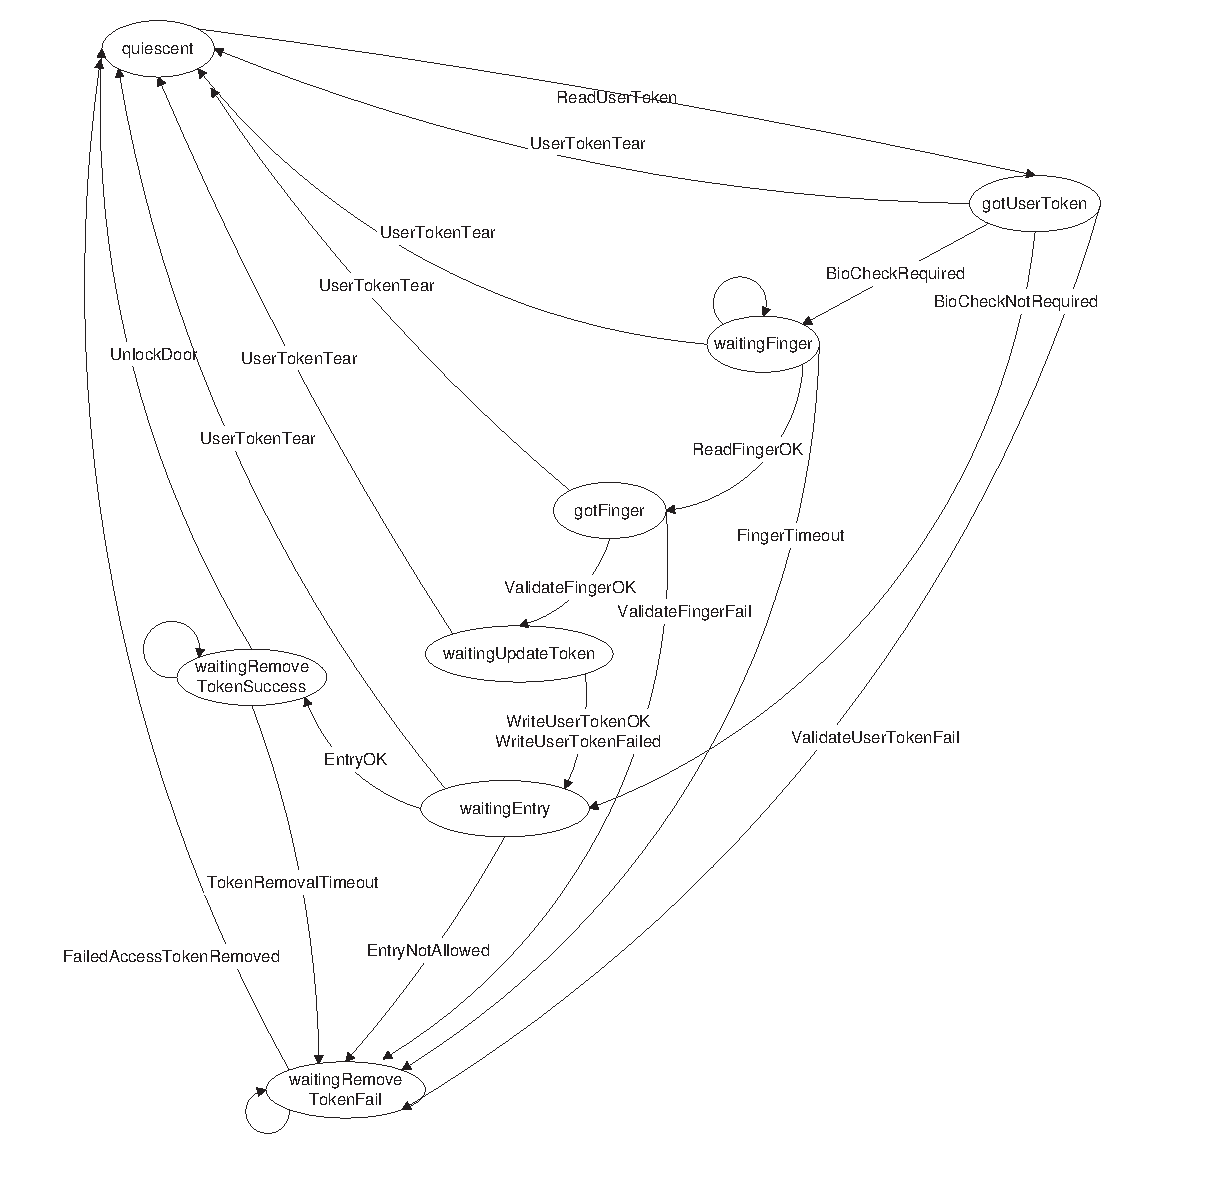
\includegraphics{50_1_entry.eps}}
    \caption{User Authentication and Entry state transitions}
    \label{fig:userEntry}
  \end{center}
\end{figure}

The process of user authentication and entry follows the following
stages:

\begin{itemize}
\item

Before any user attempts access, the system is $quiescent$.
\item
Once the token has been inserted and the information read off,
the status moves to $gotUserToken$, waiting for the system to validate
the token. 
\item
Once the token has been successfully validated the 
status moves to $waitingFinger$,
waiting for the user to give a fingerprint.
\item
Once the fingerprint has been read, the status moves to $gotFinger$,
waiting for the system to validate the fingerprint.
\item
Once a fingerprint has been successfully validated,
the status moves to $waitingUpdateToken$,
waiting to write the Auth Cert to the token.
\item
Once the Auth Cert has been written, the status moves to
$waitingEntry$, where it determines whether the role has
current entry privileges.
\item
If the role has current entry privileges the status moves to
$waitingTokenRemoveSuccess$, where the system system waits for 
the token to be removed.
\item
Once the token has been removed
the latch will be unlocked if the role has current access privileges
to the enclave and the ID Station will return to $quiescent$.
\end{itemize}
In the case of a failure in the user validation process the status
moves to  $waitingRemoveTokenFail$, waiting until the token has been removed before returning to a
$quiescent$ state.

This specification separates opening the door from having a valid Auth
Certificate. It is possible for a role to be entitled to enter the
enclave but not use the workstations (for example such clearence might
be given to a buildings maintenance engineer). TIS
configurations will ensure that having a valid Auth Certificate will
guarantee that entry to the enclave is permitted. 

\begin{traceunit}{FD.Enclave.ResetScreenMessage}
{FS.Enclave.ResetScreenMessage}
\end{traceunit}

The message displayed on the screen will indicate that the
system is busy while a user entry is in progress that blocks
administrator activity. Once the user entry activity becomes
non-blocking then an appropriate message is displayed on the screen.

\begin{schema}{ResetScreenMessageC}
        \Delta InternalC
\\      \Delta AdminC
\\      currentScreenC, currentScreenC' : ScreenC
\where
        UserEntryInProgress'
 \land currentScreenC'.screenMsgC = busyC
\\      \lor
\\      \lnot UserEntryInProgress' 
\\ \t1 \land (enclaveStatusC' = enclaveQuiescent \land rolePresentC' = \Nil 
\\ \t3          \land currentScreenC'.screenMsgC = welcomeAdminC
\\ \t2 \lor enclaveStatusC' = enclaveQuiescent \land rolePresentC' \neq \Nil 
\\ \t3          \land currentScreenC'.screenMsgC = requestAdminOpC
\\ \t2 \lor enclaveStatusC' = waitingRemoveAdminTokenFail 
\\ \t3          \land currentScreenC'.screenMsgC = removeAdminTokenC
\\ \t2 \lor enclaveStatusC' \notin 
        \{ enclaveQuiescent, waitingRemoveAdminTokenFail \} 
\\ \t3          \land currentScreenC'.screenMsgC = currentScreenC.screenMsgC)
\end{schema}

The user entry operation leaves much of the $IDStation$ state
unchanged. The context of this operation is summarised:

\begin{schema}{UserEntryContextC}
        \Delta IDStationC
\\      RealWorldChangesC
\also
        \Xi ConfigC
\\      \Xi AdminTokenC
\\      \Xi KeyStoreC
\\      \Xi AdminC
\\      \Xi KeyboardC
\\      \Xi FloppyC
\\      AddElementsToLogC
\\      LogChangeC
\\      ResetScreenMessageC
\also
      \Xi TISControlledRealWorldC
\where
        enclaveStatusC' = enclaveStatusC
\\      statusC \neq waitingEntry \implies tokenRemovalTimeoutC' = tokenRemovalTimeoutC
\\      statusC' \neq waitingFinger \implies fingerTimeout' = fingerTimeout
\also
        auditTypes~ newElements? \subseteq USER\_ENTRY\_ELEMENTS \cup USER\_INDEPENDENT\_ELEMENTS
\end{schema} 

\begin{Zcomment}
\item
The following state components may change $UserTokenC$, $InternalC$
$DoorLatchAlarmC$, $CertificateStore$, $StatsC$ and $AuditLogC$.
\item
The components of the real world controlled by TIS remain unchanged.
\item
The $tokenRemovalTimeoutC$ is only updated if the current status is
$waitingEntry$.
\item
The $fingerTimeout$ may only be updated if the current status becomes
$waitingFinger$.
\item
All elements logged during user entry operations either relate to the
user entry or are independent of any operation.
\item
Changes are logged and $newElements?$ will be added to the Audit Log.
\end{Zcomment}

Each of the following sub-operations is performed within the above context.

%----------------------------------------------------------------------
\section{User Token Tears}
%----------------------------------------------------------------------
\begin{traceunit}{FD.UserEntry.UserTokenTorn}
\traceto{FS.UserEntry.UserTokenTorn}
\end{traceunit}

During the operation the user may tear his token from the reader
prematurely. There are a number of internal states during which token
removal is deamed erroneous.

If the user tears the Token out before the operation is complete then
the operation is terminated unsuccessfully.

\begin{schema}{UserTokenTornC}
        UserEntryContextC
\also
	ClearUserToken
\\      \Xi DoorLatchAlarmC
\\      AddFailedEntryToStatsC      
\\      \Xi CertificateStore
\where
        UserHasDeparted
\\      statusC \in \{ gotUserToken, waitingUpdateToken,
waitingFinger, gotFinger, waitingEntry \}
\also
        currentDisplayC' = welcome
\\      statusC' = quiescent 
\also
        auditTypes~ newElements? \cap USER\_ENTRY\_ELEMENTS = 
        \{ userTokenRemovedElement \} 
\also
        \exists_1 element : AuditC @ element \in newElements? 
\\ \t1  \land element.elementId = userTokenRemovedElement
\\ \t1  \land element.logTime \in nowC \upto nowC'
\\ \t1  \land element.user = extractUser~ currentUserTokenC
\\ \t1  \land element.severity = warning
\\ \t1  \land element.description = noDescription

\end{schema}
\begin{Zcomment}
\item
The $userTokenRemovedElement$ is the audit entry recording that the
token has been removed from the reader outside the enclave. 
\end{Zcomment}

%-------------------------------------------------------------------
\section{Reading the User Token}
%-------------------------------------------------------------------
\begin{traceunit}{FD.UserEntry.TISReadUserToken}
\traceto{FS.UserEntry.TISReadUserToken}
\end{traceunit}


The User Entry operation is initiated when TIS is in a $quiescent$ state
and detects the presence of
a token in the user token reader (which resides outside the enclave). 

A user entry operation may start while the $enclaveStatus$ is
quiescent ($enclaveQuiescent$) or the enclave is waiting for a failed
admin token to be removed.

When the user token is first detected as present, its presence is
audited and the internal status changes. It is not until the token has 
been validated that we can be sure of the user's identity, however the
token ATR should provide a token ID which can be used as the user identity.

No other aspects of the system are modified.

\begin{schema}{GetPresentUserTokenC}
        UserEntryContextC
\also
        ReadUserTokenC
\\	\Xi DoorLatchAlarmC
\\      \Xi StatsC
\\      \Xi CertificateStore
\where
        UserEntryCanStart
\also
        userTokenPresenceC' = userTokenPresenceC
\\      currentUserTokenC' = userTokenC
\also
	currentDisplayC' = wait
\\	statusC' = gotUserToken

\also
        auditTypes~ newElements? \cap USER\_ENTRY\_ELEMENTS = 
        \{ userTokenPresentElement \} 
\also
        \exists_1 element : AuditC @ element \in newElements? 
\\ \t1  \land element.elementId = userTokenPresentElement
\\ \t1  \land element.logTime \in nowC \upto nowC'
\\ \t1  \land element.user = extractUser~ currentUserTokenC'
\\ \t1  \land element.severity = information
\\ \t1  \land element.description = noDescription

\end{schema}

The operation to read the user token is as follows:

\begin{zed}
        TISReadUserTokenC \defs GetPresentUserTokenC \hide ( newElements? )
\end{zed}


%--------------------------------------------------------------------
\section{Validating the User Token}
%--------------------------------------------------------------------
Once TIS has read a user token it must validate the contents of that
token.

A user token is valid for entry without biometric checks if the token
contains a consistent authorisation certificate which is current.

A user token is valid for entry into the enclave if the token is
consistent, current and the ID
certificate, Privilege certificate and I\&A certificate can be validated.

\begin{traceunit}{FD.UserEntry.BioCheckNotRequired}
\traceto{FS.UserEntry.BioCheckNotRequired}
\end{traceunit}

In the case where there is a
valid Authorisation certificate the biometric checks are bypassed.

\begin{schema}{BioCheckNotRequiredC}
        UserEntryContextC
\also
        \Xi UserTokenC
\\      \Xi DoorLatchAlarmC        
\\      \Xi StatsC
\\      \Xi CertificateStore
\where
        \lnot UserHasDeparted
\\      statusC = gotUserToken
\also
        UserTokenWithOKAuthCertC
\also
        statusC' = waitingEntry
\\      currentDisplayC' = wait
\also
        auditTypes~ newElements? \cap USER\_ENTRY\_ELEMENTS = 
        \{ authCertValidElement \} 
\also
        \exists_1 element : AuditC @ element \in newElements? 
\\ \t1  \land element.elementId = authCertValidElement
\\ \t1  \land element.logTime \in nowC \upto nowC'
\\ \t1  \land element.user = extractUser~ currentUserTokenC
\\ \t1  \land element.severity = information
\\ \t1  \land element.description = noDescription
\end{schema}

\begin{traceunit}{FD.UserEntry.BioCheckRequired}
\traceto{FS.UserEntry.BioCheckRequired}
\traceto{FDP\_RIP.2.1}
\end{traceunit}


The biometric checks are only required if the Authorisation
Certificate is not present or not valid. In this case the remaining
certificates on the card must be checked.

An audit element is logged indicating that the authorisation
certificate is not valid.
The audit element will reference a user, the owner of the token, there is
no additional information in the description. 

\begin{schema}{BioCheckRequiredC}
        UserEntryContextC
\also
        FlushFingerDataC
\\      \Xi UserTokenC
\\      \Xi DoorLatchAlarmC        
\\      \Xi StatsC
\\      \Xi CertificateStore
\where
        \lnot UserHasDeparted
\\      statusC = gotUserToken
\also
        \lnot UserTokenWithOKAuthCertC \land UserTokenOKC
\also
	currentDisplayC' = insertFinger
\\	statusC' = waitingFinger
\\      fingerTimeout' = currentTimeC + fingerWaitDuration
\also
        auditTypes~ newElements? \cap USER\_ENTRY\_ELEMENTS = 
        \{ authCertInvalidElement \} 
\also
        \exists_1 element : AuditC @ element \in newElements? 
\\ \t1  \land element.elementId = authCertInvalidElement
\\ \t1  \land element.logTime \in nowC \upto nowC'
\\ \t1  \land element.user = extractUser~ currentUserTokenC
\\ \t1  \land element.severity = information
\\ \t1  \land element.description = noDescription
\end{schema}

\begin{traceunit}{FD.UserEntry.ValidateUserTokenFail}
\traceto{FS.UserEntry.ValidateUserTokenFail}
\end{traceunit}

If the token cannot be validated then this is logged and the user is
required to remove the token. The audit element detailing this failure
will contain the user if this can be extracted from the token. The
description will indicate the point of failure of the card.

\begin{schema}{ValidateUserTokenFailC}
        UserEntryContextC
\also
        \Xi UserTokenC
\\      \Xi DoorLatchAlarmC        
\\      \Xi StatsC
\\      \Xi CertificateStore
\where
        \lnot UserHasDeparted
\\      statusC = gotUserToken
\also
        \lnot UserTokenOKC \land \lnot UserTokenWithOKAuthCertC
\also
	currentDisplayC' = removeToken
\\      statusC' = waitingRemoveTokenFail
\also
        auditTypes~ newElements? \cap USER\_ENTRY\_ELEMENTS = 
        \{ userTokenInvalidElement \} 
\also
        \exists_1 element : AuditC; description! : TEXT @ 
\\ \t1  element \in newElements? 
\\ \t1  \land element.elementId = userTokenInvalidElement
\\ \t1  \land element.logTime \in nowC \upto nowC'
\\ \t1  \land element.user = extractUser~ currentUserTokenC
\\ \t1  \land element.severity = warning
\\ \t1  \land (element.description = description! \land UserTokenNotOK)

\end{schema}
\begin{Zcomment}
\item
$UserTokenNotOK$ defines the error description.
\end{Zcomment}

%...............................
\subsection{Determining whether biometric checks are required}
%...............................


\begin{zed}
        DetermineBioCheckRequired \defs (BioCheckRequiredC \lor
        BioCheckNotRequiredC) \hide (newElements? )
\end{zed}

There are lots of things that may go wrong with validation of the user
token. In each case the system will terminate the operation unsuccessfully.

\begin{zed}
        TISValidateUserTokenC \defs 
                (BioCheckRequiredC 
                \lor BioCheckNotRequiredC
                \lor ValidateUserTokenFailC 
\\ \t4 \lor
        [~UserTokenTornC | statusC = gotUserToken ] ) \hide (newElements? )
\end{zed}

%-----------------------------------------------------------------
\section{Reading a fingerprint}
%----------------------------------------------------------------

\begin{traceunit}{FD.UserEntry.ReadFingerOK}
\traceto{FS.UserEntry.ReadFingerOK}
\end{traceunit}


A finger will be read if the system is currently waiting for it (has
not waited too long) and
the user Token is in place.

\begin{schema}{ReadFingerOKC}
        UserEntryContextC
\also
        \Xi DoorLatchAlarmC
\\	\Xi UserTokenC
\\      \Xi StatsC
\where
        \lnot UserHasDeparted
\\	statusC = waitingFinger
\\	fingerPresenceC = present
\\      currentTimeC \leq fingerTimeout 
\also
\\	currentDisplayC' = wait
\\	statusC' = gotFinger
\also
        auditTypes~ newElements? \cap USER\_ENTRY\_ELEMENTS = 
        \{ fingerDetectedElement \} 
\also
        \exists_1 element : AuditC @ element \in newElements? 
\\ \t1  \land element.elementId = fingerDetectedElement
\\ \t1  \land element.logTime \in nowC \upto nowC'
\\ \t1  \land element.user = extractUser~ currentUserTokenC
\\ \t1  \land element.severity = information
\\ \t1  \land element.description = noDescription
\end{schema}


\begin{traceunit}{FD.UserEntry.NoFinger}
\traceto{FS.UserEntry.NoFinger}
\end{traceunit}


If there is no finger present then, if we have not allowed sufficient
attempts to get and validate a finger, nothing happens. 

\begin{schema}{NoFingerC}
        \Xi IDStationC
\\      RealWorldChangesC
\also
        UserEntryContextC
\\      \Xi TISControlledRealWorldC
\where
        \lnot UserHasDeparted
\\      statusC = waitingFinger
\\      currentTimeC \leq fingerTimeout 
\\      fingerPresenceC = absent
\end{schema}

\begin{traceunit}{FD.UserEntry.FingerTimeout}
\traceto{FS.UserEntry.FingerTimeout}
\end{traceunit}

Alternatively, TIS may have tried to obtain a valid finger for too
long, in which case the user is requested to remove the token and 
the operation is terminated unsuccessfully. 


\begin{schema}{FingerTimeoutC}
        UserEntryContextC
\also
        \Xi UserTokenC
\\      \Xi DoorLatchAlarmC
\\      \Xi StatsC       
\where
        \lnot UserHasDeparted
\\        statusC = waitingFinger
\\      currentTimeC > fingerTimeout
\also
        currentDisplayC' = removeToken
\\      statusC' = waitingRemoveTokenFail
\also
        auditTypes~ newElements? \cap USER\_ENTRY\_ELEMENTS = 
        \{ fingerTimeoutElement \} 
\also
        \exists_1 element : AuditC @ element \in newElements? 
\\ \t1  \land element.elementId = fingerTimeoutElement
\\ \t1  \land element.logTime \in nowC \upto nowC'
\\ \t1  \land element.user = extractUser~ currentUserTokenC
\\ \t1  \land element.severity = warning
\\ \t1  \land element.description = noDescription
\end{schema}

\begin{zed}
        TISReadFingerC \defs (ReadFingerOKC \lor
        FingerTimeoutC \lor NoFingerC 
\\ \t4  \lor [~ UserTokenTornC | statusC = waitingFinger ~]) \hide (newElements?)
\end{zed}

%-------------------------------------------------------------
\section{Validating a fingerprint}
%-------------------------------------------------------------

\begin{traceunit}{FD.UserEntry.ValidateFingerOK}
\traceto{FS.UserEntry.ValidateFingerOK}
\traceto{FDP\_RIP.2.1}
\end{traceunit}

A finger must match the template information extracted from the
userToken for it to be considered acceptable.

The fingerprint being successfully validated is a prerequisite for
generating an authorisation certificate and adding it to the user token.
Validating the fingerprint is performed first.

When logging the success or otherwise of the attempt to read the
fingerprint the audit element will contain the achieved FAR if available.
\begin{axdef}
        achievedFarDescription : INTEGER32 \fun TEXT
\end{axdef}

A fingerprint is considered OK if the $verifyBio$ function returns a
successful match indication.

Following a successful match the data is flushed from the biometric
device.

\begin{schema}{ValidateFingerOKC}
	UserEntryContextC
\also
        FlushFingerDataC
\\	\Xi DoorLatchAlarmC
\\      \Xi UserTokenC
\\      \Xi CertificateStore
\\      AddSuccessfulBioCheckToStatsC
\where
        \lnot UserHasDeparted
\\	statusC = gotFinger
\also
        \exists achievedFar!, maxFar : INTEGER32 @
\\ \t1     maxFar = min \{  (extractIandACert~((goodTC \inv
                currentUserTokenC).iandACertC)).templateC.far,
        systemMaxFar \}
\\ \t1        \land (match, achievedFar!) = 
\\ \t2                verifyBio~ maxFar~ (extractIandACert~((goodTC \inv
                currentUserTokenC).iandACertC)).templateC.templateC~ fingerC 
\also
\\ \t1  \land (\exists_1 element : AuditC @ element \in newElements? 
\\ \t2  \land element.elementId = fingerMatchedElement
\\ \t2  \land element.logTime \in nowC \upto nowC'
\\ \t2  \land element.user = extractUser~ currentUserTokenC
\\ \t2  \land element.severity = information
\\ \t2  \land element.description = achievedFarDescription~ achievedFar!)
\also
	statusC' = waitingUpdateToken
\\	currentDisplayC' = wait
\also
        auditTypes~ newElements? \cap USER\_ENTRY\_ELEMENTS = 
        \{ fingerMatchedElement \} 
\end{schema}

\begin{traceunit}{FD.UserEntry.ValidateFingerFail}
\traceto{FS.UserEntry.ValidateFingerFail}
\traceto{FDP\_RIP.2.1}
\end{traceunit}


If the fingerprint is not successfully validated the user is asked to
remove their token and the entry attempt is terminated. 
The biometric check failure is recorded.

Following an unsuccessful match the data is flushed from the biometric
device.

\begin{schema}{ValidateFingerFailC}
        UserEntryContextC
\also
        FlushFingerDataC
\\	\Xi UserTokenC
\\      \Xi DoorLatchAlarmC
\\      \Xi CertificateStore
\\      AddFailedBioCheckToStatsC
\where
        \lnot UserHasDeparted
\\        statusC = gotFinger
\also
        \exists achievedFar!, maxFar : INTEGER32 @
\\ \t1     maxFar = min \{  (extractIandACert~((goodTC \inv
                currentUserTokenC).iandACertC)).templateC.far,
        systemMaxFar \}
\\ \t1        \land (noMatch, achievedFar!) = 
\\ \t2                verifyBio~ maxFar~ (extractIandACert~((goodTC \inv
                currentUserTokenC).iandACertC)).templateC.templateC~ fingerC 
\also
\\ \t1  \land (\exists_1 element : AuditC @ element \in newElements? 
\\ \t2  \land element.elementId = fingerNotMatchedElement
\\ \t2  \land element.logTime \in nowC \upto nowC'
\\ \t2  \land element.user = extractUser~ currentUserTokenC
\\ \t2  \land element.severity = warning
\\ \t2  \land element.description = achievedFarDescription~ achievedFar!)
\also
        currentDisplayC' = removeToken
\\      statusC' = waitingRemoveTokenFail
\also
        auditTypes~ newElements? \cap USER\_ENTRY\_ELEMENTS = 
        \{ fingerNotMatchedElement \} 

\end{schema}

\begin{zed}
        TISValidateFingerC \defs (ValidateFingerOKC \lor ValidateFingerFailC
\\ \t4  \lor [~ UserTokenTornC | statusC = gotFinger ~]) \hide (newElements?)
\end{zed}

%---------------------------------------------------------------------
\section{Writing the User Token}
%----------------------------------------------------------------------

The user Token will be updated with the new Auth certificate.

We implement a multi-phase design for the activity of writing the
user token. 

\begin{traceunit}{FD.UserEntry.ConstructAuthCert}
\traceto{FS.UserEntry.WriteUerTokenOK}
\traceto{FS.UserEntry.WriteUerTokenFail}
\end{traceunit}

First the authorisation certificate is constructed. 
This certificate is added to the local copy of the user Token.
This will not result in any errors since it does not require the use
of any peripherals. 


\begin{schema}{ConstructAuthCert}
	UserEntryContextC
\also
	\Xi DoorLatchAlarmC
\\      AddAuthCertToUserTokenC
\\      \Xi CertificateStore
\\      \Xi StatsC
\where
        \lnot UserHasDeparted
\\	statusC = waitingUpdateToken
\also
        statusC' = statusC
\\      currentDisplayC' = wait
\also
        auditTypes~ newElements? \cap USER\_ENTRY\_ELEMENTS = \emptyset
\end{schema}

Next the certificate will be updated.

Finally the $CertificateStore$ is updated to show the issuing of the
certificate. This will only happen if the certificate is written successfully.


\begin{traceunit}{FD.UserEntry.WriteUserTokenOK}
\traceto{FS.UserEntry.WriteUserTokenOK}
\end{traceunit}

An attempt is made to write this certificate to the token. The write of
the authorisation certificate may be successful...

\begin{schema}{WriteUserTokenOKC}
	UserEntryContextC
\also
        UpdateUserTokenC
\\	\Xi DoorLatchAlarmC
\\      \Xi UserTokenC
\\      UpdateCertificateStore
\\      \Xi StatsC
\where
        \lnot UserHasDeparted
\\	statusC = waitingUpdateToken
\also
        statusC' = waitingEntry
\\      currentDisplayC' = wait

\also
        auditTypes~ newElements? \cap USER\_ENTRY\_ELEMENTS = 
        \{ authCertWrittenElement \} 
\also
        \exists_1 element : AuditC @ element \in newElements? 
\\ \t1  \land element.elementId = authCertWrittenElement
\\ \t1  \land element.logTime \in nowC \upto nowC'
\\ \t1  \land element.user = extractUser~ currentUserTokenC
\\ \t1  \land element.severity = information
\\ \t1  \land element.description = noDescription
\end{schema}
\begin{Zcomment}
\item
Note that the decision as to whether to update the certificate store
or not can only be made once the attempt to write to the token has
been completed. Only if this write succeeds should the
$CertificateStore$ be updated.
\end{Zcomment}

\begin{traceunit}{FD.UserEntry.WriteUserTokenFail}
\traceto{FS.UserEntry.WriteUserTokenFail}
\end{traceunit}

... or may fail. The failure case models circumstances where the TIS
can detect the failure, through a write failure for instance, or a
failure to generate the certificate. 
As there is no read back of the authorisation certificate we cannot
guarantee that the audit log indicating a successful write means that
the token contains the authorisation certificate. The user will still
subsequently be admitted to the enclave if the conditions are correct. 

Whether the authorisation certificate is successfully
written or not is non-deterministic in this design since failure
conditions on signing data and writing the certificate are not modelled.   

\begin{schema}{WriteUserTokenFailC}
	UserEntryContextC
\also
        UpdateUserTokenC
\\	\Xi DoorLatchAlarmC
\\      \Xi UserTokenC
\\      \Xi StatsC
\\      \Xi CertificateStore
\where
        \lnot UserHasDeparted
\\	statusC = waitingUpdateToken
\also
        statusC' = waitingEntry
\\      currentDisplayC' = tokenUpdateFailed
\also
        auditTypes~ newElements? \cap USER\_ENTRY\_ELEMENTS = 
        \{ authCertWriteFailedElement \} 
\also
        \exists_1 element : AuditC @ element \in newElements? 
\\ \t1  \land element.elementId = authCertWriteFailedElement
\\ \t1  \land element.logTime \in nowC \upto nowC'
\\ \t1  \land element.user = extractUser~ currentUserTokenC
\\ \t1  \land element.severity = warning
\\ \t1  \land element.description = noDescription
\end{schema}

\begin{zed}
WriteUserTokenC \defs WriteUserTokenOKC \lor WriteUserTokenFailC
\end{zed}

\begin{zed}
        TISWriteUserTokenC \defs 
        (((ConstructAuthCert \hide (newElements?)) \semi WriteUserTokenC )
\\ \t4          \lor [~ UserTokenTornC | statusC = waitingUpdateToken
        ~] )  \hide ( newElements? )
\end{zed}



%------------------------------------------------------------
\section{Validating Entry}
%------------------------------------------------------------

The door will only be unlocked if the current TIS configuration allows
the user to enter the enclave at this time. It is likely that TIS
configurations will ensure that having a valid Auth Certificate will
guarantee that entry to the enclave is permitted, but such a
constraint is not specified here. 

TIS checks to ensure that the current configuration allows the user to
enter the enclave:

\begin{schema}{UserAllowedEntryC}
        UserTokenC
\\      ConfigC
\\      currentTimeC: TIME
\where
        \exists ValidTokenC @ 
\\ \t1  goodTC (\theta ValidTokenC) = currentUserTokenC
\\ \t1  \land authCertC \neq \Nil
\\ \t1  \land currentTimeC \in entryPeriodC~ (extractAuthCert~ (\The authCertC)).clearanceC.class 
\end{schema}


\begin{traceunit}{FD.UserEntry.EntryOK}
\traceto{FS.UserEntry.EntryOK}
\end{traceunit}

Only if entry is permitted at the current time will the user be
admitted to the enclave.

Note that if this stage of the processing is reached the internal
representation of the token will always contain a valid authorisation
certificate.

\begin{schema}{EntryOKC}
        UserEntryContextC
\also
        \Xi DoorLatchAlarmC
\\      \Xi UserTokenC
\\      \Xi StatsC
\\      \Xi CertificateStore
\where
         \lnot UserHasDeparted
\\        statusC = waitingEntry
\also
        UserAllowedEntryC
\also
        currentDisplayC' = openDoor
\\      statusC' = waitingRemoveTokenSuccess
\\      tokenRemovalTimeoutC' = currentTimeC + tokenRemovalDurationC

\also
        auditTypes~ newElements? \cap USER\_ENTRY\_ELEMENTS = 
        \{ entryPermittedElement \} 
\also
        \exists_1 element : AuditC @ element \in newElements? 
\\ \t1  \land element.elementId = entryPermittedElement
\\ \t1  \land element.logTime \in nowC \upto nowC'
\\ \t1  \land element.user = extractUser~ currentUserTokenC
\\ \t1  \land element.severity = information
\\ \t1  \land element.description = noDescription

\end{schema}

If the user is not allowed entry at this time they will be
requested to remove their token.

\begin{schema}{EntryNotAllowedC}
        UserEntryContextC
\also
        \Xi DoorLatchAlarmC
\\      \Xi UserTokenC
\\      \Xi StatsC      
\\      \Xi CertificateStore
\where
        \lnot UserHasDeparted
\\        statusC = waitingEntry
\also
        \lnot UserAllowedEntryC
\also
        currentDisplayC' = removeToken
\\      statusC' = waitingRemoveTokenFail
\\      tokenRemovalTimeoutC' = tokenRemovalTimeoutC
\also
        auditTypes~ newElements? \cap USER\_ENTRY\_ELEMENTS = 
        \{ entryDeniedElement \} 
\also
        \exists_1 element : AuditC @ element \in newElements? 
\\ \t1  \land element.elementId = entryDeniedElement
\\ \t1  \land element.logTime \in nowC \upto nowC'
\\ \t1  \land element.user = extractUser~ currentUserTokenC
\\ \t1  \land element.severity = warning
\\ \t1  \land element.description = noDescription

\end{schema}

\begin{zed}
        TISValidateEntryC \defs (EntryOKC
\\ \t4          \lor EntryNotAllowedC
\\ \t4          \lor [~ UserTokenTornC | statusC = waitingEntry ~])
\hide (newElements?) 
\end{zed}


%------------------------------------------------------------
\section{Unlocking the Door}
%------------------------------------------------------------

\begin{traceunit}{FD.UserEntry.UnlockDoorOK}
\traceto{FS.UserEntry.UnlockDoorOK}
\end{traceunit}


The door will only be unlocked if the current TIS configuration allows
the user to enter the enclave at this time. It is likely that TIS
configurations will ensure that having a valid Auth Certificate will
guarantee that entry to the enclave is permitted. 

The door will only be unlocked once the user has removed their token,
this helps remind the user to take their token with them.

\begin{schema}{UnlockDoorOKC}
        UserEntryContextC
\also
        UnlockDoorC
\\      ClearUserToken
\\      AddSuccessfulEntryToStatsC
\\      \Xi CertificateStore
\where
        UserHasDeparted
\\      statusC = waitingRemoveTokenSuccess
\also
        currentDisplayC' = doorUnlocked
\\      statusC' = quiescent
\end{schema}

\begin{traceunit}{FD.UserEntry.WaitingTokenRemoval}
\traceto{FS.UserEntry.WaitingTokenRemoval}
\end{traceunit}


The system will wait indefinitely for a token to be removed, however
the system will deny entry to a user who takes too long to extract
their token.

\begin{schema}{WaitingTokenRemovalC}
        \Xi IDStationC
\\      RealWorldChangesC
\also
        \Xi TISControlledRealWorldC
\where
        \lnot UserHasDeparted
\\      statusC = waitingRemoveTokenSuccess  
\\      currentTimeC \leq tokenRemovalTimeoutC 
\end{schema}
\begin{Zcomment}
\item
The constraints on this schema have been tightened as idling while
waiting for a failed token to be removed is considered part of the TIS
system idle rather than the user entry operation.
\end{Zcomment}

\begin{traceunit}{FD.UserEntry.TokenRemovalTimeout}
\traceto{FS.UserEntry.TokenRemovalTimeout}
\end{traceunit}

If the user waits too long to remove their token then this is logged
and the system continues to wait for the token to be removed but will
no longer allow access to the enclave.

\begin{schema}{TokenRemovalTimeoutC}
        UserEntryContextC
\also
        \Xi DoorLatchAlarmC
\\      \Xi UserTokenC
\\      \Xi StatsC       
\\      \Xi CertificateStore
\where
        \lnot UserHasDeparted
\\        statusC = waitingRemoveTokenSuccess
\\      currentTimeC > tokenRemovalTimeoutC 
\also
        statusC' = waitingRemoveTokenFail
\\      currentDisplayC' = removeToken
\also
        auditTypes~ newElements? \cap USER\_ENTRY\_ELEMENTS = 
        \{ entryTimeoutElement \} 
\also
        \exists_1 element : AuditC @ element \in newElements? 
\\ \t1  \land element.elementId = entryTimeoutElement
\\ \t1  \land element.logTime \in nowC \upto nowC'
\\ \t1  \land element.user = extractUser~ currentUserTokenC
\\ \t1  \land element.severity = warning
\\ \t1  \land element.description = noDescription
\end{schema}

\begin{zed}
        TISUnlockDoorC \defs (UnlockDoorOKC
        \lor  WaitingTokenRemovalC 
\\      \t2 \lor TokenRemovalTimeoutC) \hide (newElements?)
\end{zed}
 
%------------------------------------------
\section{Terminating a failed access}
%------------------------------------------

\begin{traceunit}{FD.UserEntry.FailedAccessTokenRemoved}
\traceto{FS.UserEntry.FailedAccessTokenRemoved}
\end{traceunit}

If an access attempt has failed the system waits for the token to be
removed before a new user entry operation can commence. Once the token has been
removed a new user entry may start.

The operations in the enclave are not blocked on the presence of a
failed user token in the token reader. 


\begin{schema}{FailedAccessTokenRemovedC}
        UserEntryContextC
\also
	ClearUserToken
\\      \Xi DoorLatchAlarmC
\\      AddFailedEntryToStatsC
\\      \Xi CertificateStore
\where
        UserHasDeparted
\\      statusC = waitingRemoveTokenFail
\also
        currentDisplayC' = welcome
\\      statusC' = quiescent
\also
        auditTypes~ newElements? \cap USER\_ENTRY\_ELEMENTS = 
        \{ userTokenRemovedElement \} 
\also
        \exists_1 element : AuditC @ element \in newElements? 
\\ \t1  \land element.elementId = userTokenRemovedElement
\\ \t1  \land element.logTime \in nowC \upto nowC'
\\ \t1  \land element.user = extractUser~ currentUserTokenC
\\ \t1  \land element.severity = information
\\ \t1  \land element.description = noDescription
\end{schema}


\begin{zed}
        TISCompleteFailedAccessC \defs FailedAccessTokenRemovedC  
        \hide ( newElements? )
\end{zed}

%..........................................
\section{The Complete User Entry}
%..........................................
The complete authentication process, triggered by TIS reading a User
Token, involves validating the user Token, reading and validating the
fingerprint, 
writing an authorisation certificate to the user token, waiting for
the user to remove the token, opening the door to the enclave and
in the case of a failure waiting for the system to
be in a state where it can admit another user.

\begin{zed}
        TISUserEntryOpC \defs TISReadUserTokenC 
                \lor TISValidateUserTokenC 
                \lor TISReadFingerC 
                \lor TISValidateFingerC 
\\ \t4          \lor TISWriteUserTokenC   
                \lor TISValidateEntryC 
                \lor TISUnlockDoorC 
                \lor TISCompleteFailedAccessC 
\end{zed}

This can be divided into starting a user entry:
\begin{zed}
        TISStartUserEntry \defs TISReadUserTokenC
\end{zed}

\begin{traceunit}{FD.UserEntry.ProgressUserEntry}
\traceto{FS.UserEntry.TISUserEntryOp}
\end{traceunit}

and progressing a started user entry:
\begin{zed}
        TISProgressUserEntry \defs 
                     TISValidateUserTokenC 
                \lor TISReadFingerC 
                \lor TISValidateFingerC 
\\ \t4          \lor TISWriteUserTokenC   
                \lor TISValidateEntryC 
                \lor TISUnlockDoorC 
                \lor TISCompleteFailedAccessC 
\end{zed}












%====================================================================
\chapter{Operations Within the Enclave}
\label{sec:Enclave}
%====================================================================

A number of interactions with TIS may occur within the
Enclave.
These interactions leave some of the $IDStation$ state unchanged.

\begin{schema}{EnclaveContextC}
        \Delta IDStationC
\\      RealWorldChangesC
\also
        \Xi TISControlledRealWorldC
\also
        \Xi UserTokenC
\\      \Xi FingerC
\\      \Xi StatsC
\\      \Xi CertificateStore
\\      \Xi Keyboard
\where
        fingerTimeout' = fingerTimeout
\\      tokenRemovalTimeoutC' = tokenRemovalTimeoutC
\end{schema}
\begin{Zcomment}
\item
The following state components may change $KeyStoreC$, 
$FloppyC$, $ConfigC$, $AdminC$, $InternalC$, $AdminTokenC$
$DoorLatchAlarmC$ and $AuditLogC$. 
\item
The components of the real world controlled by TIS remain unchanged.
\end{Zcomment}

The operations that may occur within the enclave include
administrator operations and the ID station enrolment. These are
described in this section.

%-------------------------------------------------------------------------
\section{Enrolment of an ID Station}
%-------------------------------------------------------------------------

\begin{traceunit}{FD.Enclave.TISEnrolOp}
\traceto{FS.Enclave.TISEnrolOp}
\end{traceunit}

Before TIS can be used it must be enrolled.

We assume
that the initial enrolment is the only possible enrolment activity.

Enrolment is a multi-phase activity, the state transistions for an
enrolment are given in Figure \ref{fig:enrol}. Before enrolment the
system is in state $notEnrolled$ and, on successful completion, it
enters the $quiescent$ state.

\begin{figure}[htbp]
  \begin{center}
    \leavevmode
    \resizebox{\textwidth}{!}{\includegraphics{50_1_enrol.eps}}
    \caption{Enrolment state transitions}
    \label{fig:enrol}
  \end{center}
\end{figure}

The context for all enrolment operations is given below.

\begin{schema}{EnrolContextC}
        EnclaveContextC
\also
        \Xi AdminC
\\      \Xi AdminTokenC
\\      \Xi DoorLatchAlarmC
\\      \Xi ConfigC
\\      \Xi FloppyC
\\      AddElementsToLogC
\\      LogChangeC
\where
        auditTypes~ newElements? \subseteq ENROL\_ELEMENTS \cup USER\_INDEPENDENT\_ELEMENTS
\end{schema}

\begin{Zcomment}
\item
The following state components may change 
$KeyStore$, $Internal$ and  $AuditLog$. 
\end{Zcomment}


%...................................
\subsection{Requesting Enrolment}
%...................................


\begin{traceunit}{FD.Enclave.RequestEnrolment}
\traceto{FS.Enclave.RequestEnrolment}
\end{traceunit}


The ID station will request enrolment while there is no Floppy
present. This will occur until a successful enrolment is achieved.

\begin{schema}{RequestEnrolmentC}
        EnrolContextC
\also
        \Xi KeyStoreC
\\      \Xi FloppyC
\where
        enclaveStatusC = notEnrolled
\\      floppyPresenceC = absent
\also
        currentScreenC'.screenMsgC = insertEnrolmentDataC
\also
        enclaveStatusC' = enclaveStatusC
\\      statusC' = statusC
\\      currentDisplayC' = blank
\also
        auditTypes~ newElements? \cap ENROL\_ELEMENTS = \emptyset
\end{schema}


\begin{traceunit}{FD.Enclave.ReadEnrolmentFloppy}
\traceto{FS.Enclave.ReadEnrolmentFloppy}
\end{traceunit}

If a floppy is present then TIS goes on to validate the
contents. Nothing is written to the log at this stage as log entries
will be made on successful or failed enrolment.

\begin{schema}{ReadEnrolmentFloppyC}
        EnrolContextC
\also
        ReadFloppyC
\\      \Xi KeyStoreC
\where
        enclaveStatusC = notEnrolled
\\      floppyPresenceC = present
\also
        currentScreenC'.screenMsgC = validatingEnrolmentDataC 
\also
        enclaveStatusC' = waitingEnrol     
\\      statusC' = statusC
\\      currentDisplayC' = blank                         
\also
        auditTypes~ newElements? \cap ENROL\_ELEMENTS = \emptyset
\end{schema}

\begin{zed}
        ReadEnrolmentDataC \defs (ReadEnrolmentFloppyC \lor
        RequestEnrolmentC) \hide (newElements? )
\end{zed}

%.........................................
\subsection{Validating Enrolment data from Floppy}
%.........................................

For the enrolment data to be acceptable the data on the floppy must be
valid enrolment data with the ID Station certificate containing this
ID station's public key. 

\begin{schema}{EnrolmentDataOKC}
        FloppyC
\\      KeyStoreC
\where
        currentFloppyC \in \ran enrolmentFileC
\\      (\exists ValidEnrolC @ \theta ValidEnrolC = enrolmentFileC \inv
currentFloppyC)
\end{schema}

\begin{traceunit}{FD.Enclave.ValidateEnrolmentDataOK}
\traceto{FS.Enclave.ValidateEnrolmentDataOK}
\end{traceunit}

If the data on the floppy is acceptable to be used for enrolment then
the Key store is updated. From this point the system is available for
use both by users entering the enclave and by administrators.

A successful enrolment is recorded in the audit log, no user can be
associated with the enrolment activity.

\begin{schema}{ValidateEnrolmentDataOKC}
        EnrolContextC
\also
        \Xi FloppyC
\\      UpdateKeyStoreFromFloppyC
\where
        enclaveStatusC = waitingEnrol
\also
        EnrolmentDataOKC
\also
        currentScreenC'.screenMsgC = welcomeAdminC
\also
        enclaveStatusC' = enclaveQuiescent 
\\      statusC' = quiescent
\\      currentDisplayC' = welcome
\also
        auditTypes~ newElements? \cap ENROL\_ELEMENTS = 
        \{ enrolmentCompleteElement \} 
\also
        \exists_1 element : AuditC @ element \in newElements? 
\\ \t1  \land element.elementId = enrolmentCompleteElement
\\ \t1  \land element.logTime \in nowC \upto nowC'
\\ \t1  \land element.user = noUser
\\ \t1  \land element.severity = information
\\ \t1  \land element.description = noDescription
\end{schema}

\begin{traceunit}{FD.Enclave.ValidateEnrolmentDataFail}
\traceto{FS.Enclave.ValidateEnrolmentDataFail}
\end{traceunit}

If the enrolment fails then TIS waits for the floppy to be removed
before prompting for new enrolment data. 

\begin{schema}{ValidateEnrolmentDataFailC}
        EnrolContextC
\also
        \Xi KeyStoreC
\\      \Xi FloppyC
\where
        enclaveStatusC = waitingEnrol
\also
        \lnot EnrolmentDataOKC
\also
        currentScreenC'.screenMsgC = enrolmentFailedC
\also
        enclaveStatusC' = waitingEndEnrol
\\      statusC' = statusC
\\      currentDisplayC' = blank
\also
        auditTypes~ newElements? \cap ENROL\_ELEMENTS = 
        \{ enrolmentFailedElement \} 
\also
        \exists_1 element : AuditC @ element \in newElements? 
\\ \t1  \land element.elementId = enrolmentFailedElement
\\ \t1  \land element.logTime \in nowC \upto nowC'
\\ \t1  \land element.user = noUser
\\ \t1  \land element.severity = warning
\end{schema}
\begin{Zcomment}
\item
The value of the $description$ is left free here as the description component of the audit element may contain
information relating to the reason that the enrolment data failed.
This is not formally stated.
\end{Zcomment}

\begin{zed}
        ValidateEnrolmentDataC \defs ValidateEnrolmentDataOKC \lor
          ValidateEnrolmentDataFailC
\end{zed}

%.........................................
\subsection{Completing a failed Enrolment}
%.........................................

A failed enrolment will only terminate once the floppy has been
removed, otherwise the system would repeatedly try to validate the
same floppy.

\begin{traceunit}{FD.Enclave.FailedEnrolFloppyRemoved}
\traceto{FS.Enclave.FailedEnrolFloppyRemoved}
\end{traceunit}


Once the floppy has been removed the administrator is prompted for
enrolment data again. We do not log the removal of the floppy in the
audit log.

\begin{schema}{FailedEnrolFloppyRemovedC}
        EnrolContextC
\also
        \Xi FloppyC
\\      \Xi KeyStoreC
\where
        enclaveStatusC = waitingEndEnrol
\\      floppyPresenceC = absent
\also
        currentScreenC'.screenMsgC = insertEnrolmentDataC
\also
        enclaveStatusC' = notEnrolled
\\      statusC' = statusC
\\      currentDisplayC' = blank
\also
        auditTypes~ newElements? \cap ENROL\_ELEMENTS = \emptyset
\end{schema}

\begin{traceunit}{FD.Enclave.WaitingFloppyRemoval}
\traceto{FS.Enclave.WaitingFloppyRemoval}
\end{traceunit}

\begin{schema}{WaitingFloppyRemovalC}
        EnclaveContextC
\also
        \Xi IDStationC
\where
        enclaveStatusC = waitingEndEnrol
\\      floppyPresenceC = present
\end{schema}

\begin{zed}
        CompleteFailedEnrolmentC \defs FailedEnrolFloppyRemovedC 
         \lor WaitingFloppyRemovalC
\end{zed}

%..........................................
\subsection{The Complete Enrolment}
%..........................................

The complete enrolment process involves reading the enrolment data,
validating it and, in the case of a failure waiting for the system to
be in a state where it can try another enrolment.

\begin{zed}
        TISEnrolOpC \defs (ReadEnrolmentDataC \lor
ValidateEnrolmentDataC 
\\      \t4 \lor CompleteFailedEnrolmentC) \hide (newElements?)
\end{zed}

%-----------------------------------------------------------------------
\section{Administrator Token Tear}
%-----------------------------------------------------------------------

The action of removing the administrator Token will result in the
administrator being logged out of the system.

This may happen at any point once a token has been inserted into the
reader. As soon as the adminitrator's token is torn this action will
be logged. 


\begin{schema}{AdminTokenTearC}
         EnclaveContextC
\\       AddElementsToLogC
\\       LogChangeC
\also
        ClearAdminToken
\\      \Xi ConfigC
\\      \Xi FloppyC
\\      ResetScreenMessageC
\where
        adminTokenPresenceC = absent
\also   
        currentScreenC'.screenMsgC = welcomeAdminC 
\\      statusC' = statusC
\\      currentDisplayC' = currentDisplayC
\also
        enclaveStatusC' = enclaveQuiescent
\end{schema}
If the admin token is torn while the system is processing an activity
within the enclave then the activity will be stopped.

\begin{schema}{BadAdminTokenTearC} 
        AdminTokenTearC
\where
        AdminHasDeparted
\\      enclaveStatusC \in \{ gotAdminToken, waitingStartAdminOp,
        waitingFinishAdminOp \} 
\also
        auditTypes~ newElements? \cap ADMIN\_ELEMENTS = 
        \{ adminTokenRemovedElement \} 
\also
        \exists_1 element : AuditC @ element \in newElements? 
\\ \t1  \land element.elementId = adminTokenRemovedElement
\\ \t1  \land element.logTime \in nowC \upto nowC'
\\ \t1  \land element.user = extractUser~ currentAdminTokenC
\\ \t1  \land element.severity = warning
\\ \t1  \land element.description = noDescription
\end{schema}


\begin{traceunit}{FD.Enclave.LoginAborted}
\traceto{FS.Enclave.LoginAborted}
\end{traceunit}

If the token is torn during the log on validation process then there
is no need to log off the administrator.

\begin{schema}{LoginAbortedC}
        BadAdminTokenTearC
\\      \Xi AdminC
\where
        enclaveStatusC = gotAdminToken
\end{schema}



%----------------------------------------------------------------------
\section{Administrator Login}
%----------------------------------------------------------------------


An Administrator logs into TIS by inserting a valid token
into the $adminToken$ reader. The authorisation certificate is
verified and the user is logged in with the privileges indicated on
the card.

Once the administrator is successfully logged into TIS, the system
records that there is a role present. The process of logging on is
given by the state transition diagram in Figure \ref{fig:logon}

\begin{figure}[htbp]
  \begin{center}
    \leavevmode
    \resizebox{\textwidth}{!}{\includegraphics{50_1_admin.eps}}
    \caption{Administrator logon state transitions}
    \label{fig:logon}
  \end{center}
\end{figure}

The context for administrator login is given below.

\begin{schema}{LoginContextC}
        EnclaveContextC
\also
        \Xi KeyStoreC
\\      \Xi DoorLatchAlarmC
\\      \Xi ConfigC
\\      AddElementsToLogC
\\      LogChangeC
\where
        statusC' = statusC
\\      currentDisplayC' = currentDisplayC
\end{schema}

\begin{Zcomment}
\item
The following state components may change 
$AdminC$, $InternalC$ and  $AuditLogC$. 
\end{Zcomment}

%..........................................
\subsection{Read Administrator Token}
%..........................................

\begin{traceunit}{FD.Enclave.GetPresentAdminToken}
\traceto{FS.Enclave.ReadAdminToken}
\end{traceunit}

When the admin token is read the action is audited and the internal
status changes. No other aspects of the system are modified.

An administrator can only log on when there is no user entry activity
in progress or TIS is waiting for a failed user token to be removed
from the token reader outside of the enclave.

\begin{schema}{GetPresentAdminTokenC}
         LoginContextC
\also
        \Xi AdminC
\\      ReadAdminTokenC
\where
        AdminLogonCanStart
\also
	enclaveStatusC' = gotAdminToken
\also
        currentScreenC' = currentScreenC
\also
        auditTypes~ newElements? \cap ADMIN\_ELEMENTS = 
        \{ adminTokenPresentElement \} 
\also
        \exists_1 element : AuditC @ element \in newElements? 
\\ \t1  \land element.elementId = adminTokenPresentElement
\\ \t1  \land element.logTime \in nowC \upto nowC'
\\ \t1  \land element.user = extractUser~ currentAdminTokenC'
\\ \t1  \land element.severity = information
\\ \t1  \land element.description = noDescription
\end{schema}

The operation to read the token is as follows:

\begin{zed}
        TISReadAdminTokenC \defs 
                GetPresentAdminTokenC \hide (newElements?)   
\end{zed}

%..........................................
\subsection{Validate Administrator Token}
%..........................................

An administrator's token is considered valid if it contains a valid
and current 
authorisation certificate. Additionally the
privileges assigned to the user within the authorisation certificate
must indicate that the user is actually an administrator.

\begin{traceunit}{FD.Enclave.ValidateAdminTokenOK}
\traceto{FS.Enclave.ValidateAdminTokenOK}
\end{traceunit}


If the token can be validated then the administrator is logged onto
TIS.

\begin{schema}{ValidateAdminTokenOKC}
        LoginContextC
\also
        \Xi AdminTokenC
\where
        \lnot AdminHasDeparted
\\      enclaveStatusC = gotAdminToken
\also
        AdminTokenOKC
\also   
        currentScreenC'.screenMsgC = requestAdminOpC 
\also
        enclaveStatusC' = enclaveQuiescent
\also
        \exists requiredRole? : ADMINPRIVILEGE @ AdminLogonC 
\\ \t1  \land requiredRole? = (extractAuthCert~ (\The (goodTC \inv
currentAdminTokenC). authCertC)).roleC 
\also
        auditTypes~ newElements? \cap ADMIN\_ELEMENTS = 
        \{ adminTokenValidElement \} 
\also
        \exists_1 element : AuditC @ element \in newElements? 
\\ \t1  \land element.elementId = adminTokenValidElement
\\ \t1  \land element.logTime \in nowC \upto nowC'
\\ \t1  \land element.user = extractUser~ currentAdminTokenC'
\\ \t1  \land element.severity = information
\\ \t1  \land element.description = noDescription
\end{schema}

\begin{traceunit}{FD.Enclave.ValidateAdminTokenFail}
\traceto{FS.Enclave.ValidateAdminTokenFail}
\end{traceunit}

If the token can not be validated then TIS waits for it to be removed.

\begin{schema}{ValidateAdminTokenFailC}
        LoginContextC
\also
        \Xi AdminTokenC
\\      \Xi AdminC
\where
        \lnot AdminHasDeparted
\\      enclaveStatusC = gotAdminToken
\also
        \lnot AdminTokenOKC
\also
        currentScreenC'.screenMsgC = removeAdminTokenC
\also
        enclaveStatusC' = waitingRemoveAdminTokenFail
\also
        auditTypes~ newElements? \cap ADMIN\_ELEMENTS = 
        \{ adminTokenInvalidElement \} 
\also
        \exists_1 element : AuditC; description! : TEXT @ 
\\ \t1  element \in newElements? 
\\ \t1  \land element.elementId = adminTokenInvalidElement
\\ \t1  \land element.logTime \in nowC \upto nowC'
\\ \t1  \land element.user = extractUser~ currentAdminTokenC'
\\ \t1  \land element.severity = warning
\\ \t1  \land element.description = description! \land AdminTokenNotOK
\end{schema}
\begin{Zcomment}
\item
$AdminTokenNotOK$ defines the value of the descriptive text applicable
based on the reason for the unacceptability of the token.
\end{Zcomment}


\begin{zed}
        TISValidateAdminTokenC \defs (ValidateAdminTokenOKC \lor
        ValidateAdminTokenFailC 
\\ \t4  \lor
        LoginAbortedC )
        \hide (newElements?)
\end{zed}

\subsection{Complete Failed Administrator Logon}

If an administrator token has failed to be accepted by TIS 
then no further actions can take place in the enclave until it has 
been removed.

\begin{traceunit}{FD.Enclave.FailedAdminTokenRemoved}
\traceto{FS.Enclave.FailedAdminTokenRemoved}
\end{traceunit}


The administrator token may be removed at any point during a user
entry, hence the context for this
activity does not place restrictions on the value of $status$.

When the admin token is removed TIS returns to a state ready
to accept another administrator logon.

\begin{schema}{FailedAdminTokenRemovedC}
        LoginContextC
\also
        \Xi AdminC
\\      ClearAdminToken
\where
        AdminHasDeparted
\\      enclaveStatusC = waitingRemoveAdminTokenFail
\also
        currentScreenC'.screenMsgC = welcomeAdminC
\also
        enclaveStatusC' = enclaveQuiescent
\also
        statusC' = statusC
\\      currentDisplayC' = currentDisplayC
\also
        auditTypes~ newElements? \cap ADMIN\_ELEMENTS = 
        \{ adminTokenRemovedElement \} 
\also
        \exists_1 element : AuditC @ element \in newElements? 
\\ \t1  \land element.elementId = adminTokenRemovedElement
\\ \t1  \land element.logTime \in nowC \upto nowC'
\\ \t1  \land element.user = extractUser~ currentAdminTokenC
\\ \t1  \land element.severity = information
\\ \t1  \land element.description = noDescription
\end{schema}

The case where the token is not removed will be captured within the
model of the system being idle.

\begin{zed}
        TISCompleteFailedAdminLogonC \defs FailedAdminTokenRemovedC 

\end{zed}

%...............................................
\subsection{The Complete Administrator Logon}
%...............................................

\begin{traceunit}{FD.Enclave.TISAdminLogin}
\traceto{FS.Enclave.TISAdminLogin}
\end{traceunit}

The complete administrator logon process, from the point that the
system has detected the presence of a token in the administrator
reader, involves 
validating the administrator token and, in the case of a failure 
waiting for the system to be in a state where it can try another logon.

\begin{zed}
        TISAdminLogonC \defs TISReadAdminTokenC \lor
        TISValidateAdminTokenC \lor TISCompleteFailedAdminLogonC 
\end{zed}

This can be divided into starting the administrator logon:
\begin{zed}
        TISStartAdminLogonC \defs TISReadAdminTokenC  
\end{zed}
 
and progressing the logon to completion. 
\begin{zed}
        TISProgressAdminLogon \defs 
        TISValidateAdminTokenC \lor TISCompleteFailedAdminLogonC 
\end{zed}

%-----------------------------------------------------------------
\section{Administrator Logout}
\label{sec:AdminLogout}
%-----------------------------------------------------------------

Administrator logout can be achieved in two ways, either the
administrator removes their token from TIS, or the Authorisation
certificate on the token expires, causing the system to automatically
log off the administrator.

\begin{traceunit}{FD.Enclave.AdminLogout}
\traceto{FS.Enclave.AdminLogout}
\end{traceunit}

If TIS is not performing an administrator operation then the
token may be removed to log out the administrator.

\begin{schema}{TokenRemovedAdminLogoutC}
        AdminTokenTearC
\\      AdminLogoutC
\also
        ClearAdminToken
\where        
        PresentAdminHasDeparted
\\      enclaveStatusC = enclaveQuiescent
\also
        auditTypes~ newElements? \cap ADMIN\_ELEMENTS = 
        \{ adminTokenRemovedElement \} 
\also
        \exists_1 element : AuditC @ element \in newElements? 
\\ \t1  \land element.elementId = adminTokenRemovedElement
\\ \t1  \land element.logTime \in nowC \upto nowC'
\\ \t1  \land element.user = extractUser~ currentAdminTokenC
\\ \t1  \land element.severity = information
\\ \t1  \land element.description = noDescription
\end{schema}


\begin{traceunit}{FD.Enclave.BadAdminLogout}
\traceto{FS.Enclave.BadAdminLogout}
\end{traceunit}

If the administrator is performing an operation (other than shutdown) when the token is torn
then the administrator will be logged off.

\begin{schema}{BadAdminLogoutC}
        BadAdminTokenTearC
\\      AdminLogoutC
\where
        PresentAdminHasDeparted
\\      enclaveStatusC \in \{ waitingStartAdminOp, waitingFinishAdminOp
        \}
\end{schema}

\begin{traceunit}{FD.Enclave.AdminTokenTimeout}
\traceto{FS.Enclave.AdminTokenTimeout}
\end{traceunit}


The TIS will automatically logout an administrator whose token
expires. This occurs if the validity period on the Authorisation
certificate expires.

\begin{schema}{AdminTokenTimeoutC}
        LoginContextC
\also
        AdminLogoutC
\\      AddElementsToLogC
\\      ResetScreenMessageC
\where
        AdminTokenHasExpired
\also
        enclaveStatusC' = waitingRemoveAdminTokenFail
\also
        auditTypes~ newElements? \cap ADMIN\_ELEMENTS = 
        \{ adminTokenExpiredElement \} 
\also
        \exists_1 element : AuditC @ element \in newElements? 
\\ \t1  \land element.elementId = adminTokenExpiredElement
\\ \t1  \land element.logTime \in nowC \upto nowC'
\\ \t1  \land element.user = extractUser~ currentAdminTokenC
\\ \t1  \land element.severity = warning
\\ \t1  \land element.description = noDescription
\end{schema}

\begin{traceunit}{FD.Enclave.TISCompleteTimeoutAdminLogout}
\traceto{FS.Enclave.TISCompleteTimeoutAdminLogout}
\end{traceunit}

If the administrator's token expires then it must be removed before
further activities can take place at the TIS console. The behaviour
and conditions are identical to the behaviour when the system waits for a the
administrator to remove their token following a failed logon.

\begin{zed}
TISCompleteTimeoutAdminLogoutC \defs TISCompleteFailedAdminLogonC
\end{zed}

%...........................
\subsection{Complete Administrator Logout}
%............................

\begin{traceunit}{FD.Enclave.TISAdminLogout}
\traceto{FS.Enclave.TISAdminLogout}
\end{traceunit}

The complete administrator logout process which must be performed as
soon as an Administrator needs to be logged out is given below.

\begin{zed}
        TISAdminLogoutC \defs ( TokenRemovedAdminLogoutC \lor
        AdminTokenTimeoutC  
\\ \t4  \lor  BadAdminLogoutC ) \hide (newElements?)
\end{zed}



%-----------------------------------------------------------------
\section{Administrator Operations}
%-----------------------------------------------------------------
An administrator operation can take place as long as an administrator
is present. The operation is started by receiving a valid request to
perform an operation from the keyboard. TIS will ensure that the
requested operation is one compatible with the current role present.

Once the operation is started the behaviour depends on the type of
operation. Operations are either short, and can be implemented in one
phase or they are multi-phase operations. 

$shutdown$ and $overrideLock$ are short operations, while $archiveLog$
and $updateCofigData$ are multi phase operations.

The state transition diagram for administrator operations is given in
Figure \ref{fig:adminOp}

\begin{figure}[htbp]
  \begin{center}
    \leavevmode
    \resizebox{\textwidth}{!}{\includegraphics{50_1_adminOp.eps}}
    \caption{Administrator operation state transitions}
    \label{fig:adminOp}
  \end{center}
\end{figure}

All administrator operations have a common context, in which the
$AdminToken$ does not change.
An administrator can only perform an operation when there is no user 
entry activity
in progress or TIS is waiting for a failed user token to be removed
from the token reader outside of the enclave.


\begin{schema}{AdminOpContextC}
        EnclaveContextC
\also
        \Xi KeyStoreC
\\      \Xi AdminTokenC
\\      AddElementsToLogC
\\      LogChangeC
\end{schema}
\begin{Zcomment}
\item
The following state components may change   
$FloppyC$, $ConfigC$, $AdminC$, $DoorLatchAlarmC$ and $AuditLogC$. 
\end{Zcomment}

Once an operation has been started its context is given by:

\begin{schema}{AdminOpStartedContextC}
        AdminOpContextC
\where
        \lnot AdminHasDeparted
\\      enclaveStatusC = waitingStartAdminOp
\also
        statusC' = statusC
\end{schema}

Some operations are multi-phase, the context for completing a
multi-phase operation is given by: 

\begin{schema}{AdminOpFinishContextC}
        AdminOpContextC
\also
        AdminFinishOpC
\where
        \lnot AdminHasDeparted
\\      enclaveStatusC = waitingFinishAdminOp
\also
        statusC' = statusC
\\      currentDisplayC' = currentDisplayC
\also
        enclaveStatusC' = enclaveQuiescent
\end{schema}


%-----------------------------------------------------------------
\section{Starting Operations}
%-----------------------------------------------------------------


All administrator operations are initiated in the same way. This
involves validating the latest keyboard input and determining whether
it is a valid operation request.

TIS only attempts to start an operation if there is an administrator
present and there is no current activity in the enclave.
An administrator can only start an operation when there is no user
entry activity in progress or TIS is waiting for a failed user token 
to be removed from the token reader outside of the enclave.

\begin{schema}{StartOpContextC}
        EnclaveContextC
\also
        \Xi DoorLatchAlarmC
\\      \Xi ConfigC
\\      \Xi FloppyC
\\      \Xi KeyStoreC
\\      \Xi AdminTokenC
\\      AddElementsToLogC
\\      LogChangeC
\where
        AdminOpCanStart        
\also
        statusC' = statusC
\\      currentDisplayC' = currentDisplayC
\end{schema}
\begin{Zcomment}
\item
The following state components may change  
$InternalC$, $AdminC$ and $AuditLogC$. 
\item
We strengthen the precondition of this context to give priority to
starting a
user entry over starting an administrator operation.
\end{Zcomment}

%..........................................
\subsection{Validating an Operation Request}
%..........................................

\begin{traceunit}{FD.Enclave.ValidateOpRequestOK}
\traceto{FS.Enclave.ValidateOpRequestOK}
\end{traceunit}

Once the data from the keyboard has been read this must be validated
to ensure it corresponds to a valid operation.

\begin{axdef}
        keyedDataText : KEYBOARD \fun TEXT
\end{axdef}

\begin{schema}{ValidateOpRequestOKC}
        StartOpContextC
\where
        keyedDataPresenceC = present
\\      \exists request? : KEYBOARD @ request? = keyboardC \land
AdminOpIsAvailable 
\also
        currentScreenC'.screenMsgC = doingOpC
\also
        enclaveStatusC' = waitingStartAdminOp
\also
        \exists requestedOp? : ADMINOP @ requestedOp? = keyedOps \inv
        keyboardC 
\\ \t1  \land AdminStartOpC 
\also
        auditTypes~ newElements? \cap ADMIN\_ELEMENTS = 
        \{ operationStartElement \} 
\also
        \exists_1 element : AuditC @ element \in newElements? 
\\ \t1  \land element.elementId = operationStartElement
\\ \t1  \land element.logTime \in nowC \upto nowC'
\\ \t1  \land element.user = extractUser~ currentAdminTokenC
\\ \t1  \land element.severity = information
\\ \t1  \land element.description = keyedDataText~ keyboardC
\end{schema}

\begin{traceunit}{FD.Enclave.ValidateOpRequestFail}
\traceto{FS.Enclave.ValidateOpRequestFail}
\end{traceunit}


If the data from the keyboard doesn't correspond to an operation that
can be performed at present then the operation is not started and the
attempt to start an illegal operation is logged.

\begin{schema}{ValidateOpRequestFailC}
        StartOpContextC
\also
        \Xi AdminC
\where
        keyedDataPresenceC = present
\\      \exists request? : KEYBOARD @ request? = keyboardC \land
\lnot AdminOpIsAvailable 
\also
        currentScreenC'.screenMsgC = invalidRequestC
\also
        enclaveStatusC' = enclaveStatusC
\also
        auditTypes~ newElements? \cap ADMIN\_ELEMENTS = 
        \{ invalidOpRequestElement \} 
\also
        \exists_1 element : AuditC @ element \in newElements? 
\\ \t1  \land element.elementId = invalidOpRequestElement
\\ \t1  \land element.logTime \in nowC \upto nowC'
\\ \t1  \land element.user = extractUser~ currentAdminTokenC
\\ \t1  \land element.severity = warning
\\ \t1  \land element.description = keyedDataText~ keyboardC
\end{schema}

\begin{traceunit}{FD.Enclave.NoOpRequest}
\traceto{FS.Enclave.NoOpRequest}
\end{traceunit}


If there is no data at the keyboard then TIS waits for user interaction.

\begin{schema}{NoOpRequestC}
        StartOpContextC
\also
        \Xi IDStationC
\where
        keyedDataPresenceC = absent
\end{schema}

\begin{zed}
        ValidateOpRequestC \defs ValidateOpRequestOKC \lor
        ValidateOpRequestFailC \lor NoOpRequestC
\end{zed}

\subsection{Complete Operation Start}
\begin{traceunit}{FD.Enclave.TISStartAdminOp}
\traceto{FS.Enclave.TISStartAdminOp}
\end{traceunit}


The process of starting an administrator operation involves exactly the validation of an
operation request.

\begin{zed}
        TISStartAdminOpC \defs ValidateOpRequestC
\end{zed}


%-------------------------------------------------------------------
\section{Archiving the Log}
%-------------------------------------------------------------------


When the log is archived it is copied to floppy and the internally
held log is truncated.

The internally held log can only be truncated if the write to floppy
succeeds.  

To check that the archive succeeded the floppy is read back and the
data compared with that held by the system.

This is a two phase operation, during the first phase the log is
written to floppy, during the second phase the data on the floppy is
validated. 


%............................
\subsection{Writing the archive Log}
%............................

\begin{traceunit}{FD.Enclave.StartArchiveLogOK}
\traceto{FS.Enclave.StartArchiveLogOK}
\end{traceunit}

The first phase of this operation is to write the archive log to
floppy.

\begin{schema}{StartArchiveLogOKC}
        EnclaveContextC
\also
        \Xi AdminTokenC
\\      \Xi KeyboardC
\\      \Xi KeyStoreC
\\      \Xi Config
\\      \Xi Admin
\\      \Xi AdminToken     
\\      LogChangeC
\also
        newElements? : \finset AuditC
 \where
     \lnot AdminHasDeparted
 \\     enclaveStatusC = waitingStartAdminOp
\also
        \The currentAdminOpC = archiveLog
\\      floppyPresenceC = present
\also
        floppyPresenceC' = floppyPresenceC
\\      currentFloppyC' = currentFloppyC
\also
        currentScreenC'.screenMsgC = doingOpC
\also
        statusC' = statusC
\also
        enclaveStatusC' = waitingFinishAdminOp
\\      (\exists archive! : \finset AuditC @ ArchiveLogC \land
writtenFloppyC' = auditFileC~ archive! )
\end{schema}
\begin{Zcomment}
\item
Note this operation makes other altertions to the audit log so cannot use
the $AdminOpStartedContext$.
\end{Zcomment}
We wait indefinitely for a floppy to be present.

\begin{traceunit}{FD.Enclave.StartArchiveLogWaitingFloppy}
\traceto{FS.Enclave.StartArchiveLogWaitingFloppy}
\end{traceunit}

\begin{schema}{StartArchiveLogWaitingFloppyC}
        AdminOpStartedContextC
\also   
        \Xi ConfigC
\\      \Xi AdminC    
\\      \Xi FloppyC
\where
        \The currentAdminOpC = archiveLog
\\      floppyPresenceC = absent
\also
        currentScreenC'.screenMsgC = insertBlankFloppyC
\\      currentDisplayC' = currentDisplayC
\also
        enclaveStatusC' = enclaveStatusC
\end{schema}

\begin{zed}
        StartArchiveLogC \defs ((StartArchiveLogOKC \semi UpdateFloppyC) 
\\ \t4                  \lor StartArchiveLogWaitingFloppyC  ) \hide
                        (newElements? )
\end{zed}


%............................
\subsection{Clearing the archive Log}
%............................

Note this operation makes altertions to the audit log other than the
addition of elements so cannot use
the $AdminOpFinishContext$. We define a specific context for
completing the archive log.

\begin{schema}{FinishArchiveLogContext}
        EnclaveContextC
\also
        \Xi AdminTokenC
\\      \Xi KeyboardC
\\      \Xi KeyStoreC
\\      \Xi ConfigC
\\      AdminFinishOpC     
\\      \Xi DoorLatchAlarmC
\\      LogChangeC
\where
        statusC' = statusC
\\      currentDisplayC' = currentDisplayC
\also
        enclaveStatusC' = enclaveQuiescent
\end{schema}


\begin{traceunit}{FD.Enclave.FinishArchiveLogOK}
\traceto{FS.Enclave.FinishArchiveLogOK}
\end{traceunit}

The audit log is only truncated after a check has been made to ensure
that the actual floppy data matches what the system believes is on the
floppy. 

\begin{schema}{FinishArchiveLogOKC}
        FinishArchiveLogContext
\also
        ReadFloppyC
\\      ClearLogC
\where
        \lnot AdminHasDeparted
\\      enclaveStatusC = waitingFinishAdminOp
\\      \The currentAdminOpC = archiveLog
\\      floppyPresenceC = present
\also
        writtenFloppyC = currentFloppyC'
\also
        currentScreenC'.screenMsgC = requestAdminOpC
\end{schema}



\begin{traceunit}{FD.Enclave.FinishArchiveLogNoFloppy}
\traceto{FS.Enclave.FinishArchiveLogNoFloppy}
\end{traceunit}

If the administrator is impatient and removes the floppy early then
the archive fails as the system cannot check that the archive was taken.

The audit log entry for this failure is distinguished from the failure
caused by the written data failing to match by the descriptive text in
the audit record.

\begin{axdef}
        floppyRemoved, floppyHasBadData : TEXT
\end{axdef}

\begin{schema}{FinishArchiveLogNoFloppyC}
        FinishArchiveLogContext
\also
        CancelArchive
\\      \Xi FloppyC
\where
       \The currentAdminOpC = archiveLog
\\      floppyPresenceC = absent
\also
        currentScreenC'.screenMsgC = archiveFailedC
\also
        auditTypes~ newElements? \cap ADMIN\_ELEMENTS = 
        \{ archiveCheckFailedElement \} 
\also
        \exists_1 element : AuditC @ element \in newElements? 
\\ \t1  \land element.elementId = archiveCheckFailedElement
\\ \t1  \land element.logTime \in nowC \upto nowC'
\\ \t1  \land element.user = extractUser~ currentAdminTokenC
\\ \t1  \land element.severity = warning
\\ \t1  \land element.description = floppyRemoved
\end{schema}


\begin{traceunit}{FD.Enclave.FinishArchiveLogBadMatch}
\traceto{FS.Enclave.FinishArchiveLogBadMatch}
\end{traceunit}

If the data read back from the floppy does not match what the ID
station believes should be on the floppy then the archive fails.

\begin{schema}{FinishArchiveLogBadMatchC}
        FinishArchiveLogContext
\also
        CancelArchive
\\      ReadFloppyC
\where
        \The currentAdminOpC = archiveLog
\\      floppyPresenceC = present
\also
        writtenFloppyC \neq currentFloppyC'
\also
        currentScreenC'.screenMsgC = archiveFailedC
\also
        auditTypes~ newElements? \cap ADMIN\_ELEMENTS = 
        \{ archiveCheckFailedElement \} 
\also
        \exists_1 element : AuditC @ element \in newElements? 
\\ \t1  \land element.elementId = archiveCheckFailedElement
\\ \t1  \land element.logTime \in nowC \upto nowC'
\\ \t1  \land element.user = extractUser~ currentAdminTokenC
\\ \t1  \land element.severity = warning
\\ \t1  \land element.description = floppyHasBadData
\end{schema}

\begin{zed}
        FinishArchiveLogFailC \defs FinishArchiveLogBadMatchC \lor
        FinishArchiveLogNoFloppyC
\also
        FinishArchiveLogC \defs (FinishArchiveLogOKC \lor FinishArchiveLogFailC
         ) \hide (newElements?)
\end{zed}

%............................
\subsection{The complete archive Log operation}
%............................

\begin{traceunit}{FD.Enclave.TISArchiveLogOp}
\traceto{FS.Enclave.TISArchiveLogOp}
\end{traceunit}


Combining the start and finish phase of this operation gives the
complete operation.
\begin{zed}
        TISArchiveLogOpC \defs StartArchiveLogC \lor FinishArchiveLogC
\end{zed}


%-------------------------------------------------------------------
\section{Updating Configuration Data}
%-------------------------------------------------------------------

The operation to update the configuration data is a two phase
operation. During the first phase the configuration data is read from
floppy. During the second phase the configuration data provided on the
floppy is checked (currently the check is purely that the data is
configuration data) and the TIS configuration data is replaced by the
new data.


%..........................................
\subsection{Reading Configuration Data}
%..........................................

\begin{traceunit}{FD.Enclave.StartUpdateConfigDataOK}
\traceto{FS.Enclave.StartUpdateConfigDataOK}
\end{traceunit}


In order to update configuration data the administrator must supply
replacement configuration data on a floppy disk.


\begin{schema}{StartUpdateConfigOKC}
        AdminOpStartedContextC
\also   
        ReadFloppyC
\\      \Xi ConfigC
\\      \Xi AdminC     
\\      \Xi DoorLatchAlarmC
\where
       \The currentAdminOpC = updateConfigData
\\      floppyPresenceC = present
\also
        currentScreenC'.screenMsgC = doingOpC
\\      currentDisplayC' = currentDisplayC
\also
        enclaveStatusC' = waitingFinishAdminOp
\end{schema}

\begin{traceunit}{FD.Enclave.StartUpdateConfigWaitingFloppy}
\traceto{FS.Enclave.StartUpdateConfigWaitingFloppy}
\end{traceunit}


We wait indefinitely for a floppy to be present.

\begin{schema}{StartUpdateConfigWaitingFloppyC}
        AdminOpStartedContextC
\also   
        \Xi FloppyC    
\\      \Xi ConfigC
\\      \Xi AdminC 
\\      \Xi DoorLatchAlarmC
\where
        \The currentAdminOpC = updateConfigData
\\      floppyPresenceC = absent
\also
        currentScreenC'.screenMsgC = insertConfigDataC
\\      currentDisplayC' = currentDisplayC
\also
        enclaveStatusC' = enclaveStatusC
\end{schema}

\begin{zed}
        StartUpdateConfigDataC \defs (StartUpdateConfigOKC  
         \lor StartUpdateConfigWaitingFloppyC ) \hide
(newElements? )
\end{zed}

%..........................................
\subsection{Storing Configuration Data}
%..........................................

\begin{traceunit}{FD.Enclave.FinishUpdateConfigDataOK}
\traceto{FS.Enclave.FinishUpdateConfigDataOK}
\end{traceunit}



The supplied data will be used to replace the current configuration data
if it is valid configuration data.

\begin{schema}{FinishUpdateConfigDataOKC}
        AdminOpFinishContextC
\also
        \Xi FloppyC
\\      \Xi DoorLatchAlarmC
\where
        \The currentAdminOpC = updateConfigData
\also        
        currentFloppyC \in \ran configFileC
\also
        \theta ConfigC' = configFileC \inv currentFloppyC
\also
        currentScreenC'.screenMsgC = requestAdminOpC
\also
        auditTypes~ newElements? \cap ADMIN\_ELEMENTS = 
        \{ updatedConfigDataElement \} 
\also
        \exists_1 element : AuditC @ element \in newElements? 
\\ \t1  \land element.elementId = updatedConfigDataElement
\\ \t1  \land element.logTime \in nowC \upto nowC'
\\ \t1  \land element.user = extractUser~ currentAdminTokenC
\\ \t1  \land element.severity = information
\end{schema}
\begin{Zcomment}
\item
The description within the audit element should summarise the new
configuration data values. This is not formally stated here so the
value of the description is left free.
\end{Zcomment}

\begin{traceunit}{FD.Enclave.FinishUpdateConfigDataFail}
\traceto{FS.Enclave.FinishUpdateConfigDataFail}
\end{traceunit}


If the supplied data is not valid configuration data the operation
terminates without changing the TIS configuration data.

\begin{schema}{FinishUpdateConfigDataFailC}
        AdminOpFinishContextC
\also
        \Xi ConfigC
\\      \Xi FloppyC
\\      \Xi DoorLatchAlarmC
\where
        \The currentAdminOpC = updateConfigData
\also        
        currentFloppyC \notin \ran configFileC
\also
        currentScreenC'.screenMsgC = invalidDataC
\also
        auditTypes~ newElements? \cap ADMIN\_ELEMENTS = 
        \{ invalidConfigDataElement \} 
\also
        \exists_1 element : AuditC @ element \in newElements? 
\\ \t1  \land element.elementId = invalidConfigDataElement
\\ \t1  \land element.logTime \in nowC \upto nowC'
\\ \t1  \land element.user = extractUser~ currentAdminTokenC
\\ \t1  \land element.severity = warning
\\ \t1  \land element.description = noDescription
\end{schema}

\begin{zed}
        FinishUpdateConfigDataC \defs ( FinishUpdateConfigDataOKC \lor
        FinishUpdateConfigDataFailC ) \hide
( newElements? )
\end{zed}

%............................
\subsection{The complete update configuration data operation}
%............................

\begin{traceunit}{FD.Enclave.TISUpdateConfigDataOp}
\traceto{FS.Enclave.TISUpdateConfigDataOp}
\end{traceunit}



Combining the start and finish phase of this operation gives the
complete operation.

\begin{zed}
        TISUpdateConfigDataOpC \defs StartUpdateConfigDataC \lor FinishUpdateConfigDataC
\end{zed}

%---------------------------------------------------------------------
\section{Shutting Down the ID Station}
%---------------------------------------------------------------------


Shutting down the ID Station is a single phase operation.

When the ID Station is shutdown the door is automatically locked so
the system is in a secure state. The ID Station cannot be shutdown if
the door is currently open, this prevents the enclave being left in an
insecure state once TIS is shutdown.

\begin{traceunit}{FD.Enclave.ShutdownOK}
\traceto{FS.Enclave.ShutdownOK}
\end{traceunit}


\begin{schema}{ShutdownOKC}
        \Delta IDStationC
\\      RealWorldChangesC
\also
        \Xi TISControlledRealWorldC
\also   
        ClearUserToken
\\      ClearAdminToken
\\      \Xi FingerC
\\      \Xi StatsC
\\      \Xi CertificateStore
\\      \Xi Keyboard
\\      \Xi KeyStore
\\      \Xi ConfigC
\\      \Xi FloppyC
\\      LockDoorC
\\      AdminLogoutC
\\      AddElementsToLogC
\where
        enclaveStatusC = waitingStartAdminOp
\\      \The currentAdminOpC = shutdownOp
\\      currentDoorC = closed
\also
        currentScreenC'.screenMsgC = clearC
\also
        enclaveStatusC' = shutdown
\\      currentDisplayC' = blank
\also
        auditTypes~ newElements? \cap ADMIN\_ELEMENTS = 
        \{ shutdownElement \} 
\also
        \exists_1 element : AuditC @ element \in newElements? 
\\ \t1  \land element.elementId = shutdownElement
\\ \t1  \land element.logTime \in nowC \upto nowC'
\\ \t1  \land element.user = extractUser~ currentAdminTokenC
\\ \t1  \land element.severity = information
\\ \t1  \land element.description = noDescription
\end{schema}
\begin{Zcomment}
\item
This operation cannot be aborted by the administrator tearing their
token, hence the $AdminOpStartedContextC$ cannot be used here.
\end{Zcomment}

\begin{traceunit}{FD.Enclave.ShutdownWaitingDoor}
\traceto{FS.Enclave.ShutdownWaitingDoor}
\end{traceunit}

TIS waits indefinitely for the door to be closed before completing the shutdown.

\begin{schema}{ShutdownWaitingDoorC}
        AdminOpContextC
\also   
\\      \Xi ConfigC
\\      \Xi FloppyC
\\      \Xi DoorLatchAlarmC
\\      \Xi AdminC
\where
        enclaveStatusC = waitingStartAdminOp
\\      \The currentAdminOpC = shutdownOp
\\      currentDoorC = open
\also
        currentScreenC'.screenMsgC = closeDoorC
\also
        statusC' = statusC
\\      enclaveStatusC' = enclaveStatusC
\\      currentDisplayC' = currentDisplayC
\end{schema}

\begin{traceunit}{FD.Enclave.TISShutdownOp}
\traceto{FS.Enclave.TISShutdownOp}
\end{traceunit}

There is nothing that can go wrong with the shutdown operation.

\begin{zed}
        TISShutdownOpC \defs (ShutdownOKC \lor ShutdownWaitingDoorC)
        \hide (newElements?)
\end{zed}

%-----------------------------------------------------------------------
\section{Unlocking the Enclave Door}
%-----------------------------------------------------------------------

Unlocking the enclave door is a single phase operation.

\begin{traceunit}{FD.Enclave.OverrideDoorLockOK}
\traceto{FS.Enclave.OverrideDoorLockOK}
\end{traceunit}

A guard may need to open the enclave door to admit someone who cannot
be admitted by the system.

\begin{schema}{OverrideDoorLockOKC}
        AdminOpStartedContextC
\also   
        \Xi FloppyC
\\      \Xi ConfigC
\\      AdminFinishOpC
\\      UnlockDoorC
\where
        \The currentAdminOpC = overrideLock
\also
        currentScreenC'.screenMsgC = requestAdminOpC
\\      currentDisplayC' = doorUnlocked
\also
        enclaveStatusC' = enclaveQuiescent
\also
        auditTypes~ newElements? \cap ADMIN\_ELEMENTS = 
        \{ overrideLockElement \} 
\also
        \exists_1 element : AuditC @ element \in newElements? 
\\ \t1  \land element.elementId = overrideLockElement
\\ \t1  \land element.logTime \in nowC \upto nowC'
\\ \t1  \land element.user = extractUser~ currentAdminTokenC
\\ \t1  \land element.severity = information
\\ \t1  \land element.description = noDescription
\end{schema}

\begin{traceunit}{FD.Enclave.TISUnlockDoorOp}
\traceto{FS.Enclave.TISUnlockDoorOp}
\end{traceunit}

This operation has no failures, other than the administrator tearing
their token before the operation completes, the token tear is covered
in Section \ref{sec:AdminLogout}.

\begin{zed}
        TISOverrideDoorLockOpC \defs ( OverrideDoorLockOKC ) \hide
(newElements? )
\end{zed}





%=========================================================================
\chapter{The Initial System and Startup}
\label{sec:Start}
%=========================================================================
\section{The Initial System}
%----------------------------------

\begin{traceunit}{FD.TIS.InitIDStation}
\traceto{FS.TIS.InitIDStation}
\end{traceunit}

After initial installation the system has the following properties
\begin{itemize}
\item
an empty key store, which means it is unable to authorise entry to anyone;
\item
default configuration data, which does not permit entry to anyone;
\item
the door latched;
\item
an empty audit log;
\item
the internal times all set to zero (a time before the current time).
\end{itemize}

The door is assumed closed at initialisation, this ensures that the alarm
will not sound before the first time that data is polled.

\begin{schema}{InitDoorLatchAlarmC}
        DoorLatchAlarmC
\where
	currentTimeC = zeroTime
\\	currentDoorC = closed
\\	latchTimeoutC = zeroTime
\\	alarmTimeoutC = zeroTime
\\      doorAlarmC = silent
\\      currentLatchC = locked
\end{schema}

There are no keys held by the system.

\begin{schema}{InitKeyStoreC}
        KeyStoreC
\where
        keys = \emptyset
\end{schema}

The initial certificate store has the 0 as the available serial number.

\begin{schema}{InitCertificateStore}
        CertificateStore
\where
        nextSerialNumber = 0
\end{schema}        


This default configuration assumes the lowest classification possible
for the enclave. This ensures that it does not give inadvertently
high clearance to the authorisation certificate. The parameters that
define the $authPeriod$
and $entryPeriod$ functions are set to enable entry into the enclave
to re-configure the TIS. This configuration will
allow Auth Certificates to be generated with a validity of 2 hours
from the point of issue.
\begin{schema}{InitConfigC}
        ConfigC
\where
	alarmSilentDurationC = 10
\\      latchUnlockDurationC = 150
\\      tokenRemovalDurationC = 100
\\      fingerWaitDuration = 100
\\      enclaveClearanceC = unmarked
\\      minEntryClass = unmarked
\also   
        maxAuthDuration = 72000
\\      accessPolicy = allHours
\\      systemMaxFar = 1000
\end{schema}
\begin{Zcomment}
\item 
The initial values of $workingHoursStart$, $workingHoursEnd$ will not
impact the entry or authorisation periods so are not defined here,
they are free to be implemented with any value.
\end{Zcomment} 

Initially no administrator is logged on and no administator operations
are taking place.
\begin{schema}{InitAdminC}
        AdminC
\where
        rolePresentC = \Nil
\\      currentAdminOpC = \Nil
\end{schema}

Initially the statistics are set to zero, indicating no use of the
system to date.
\begin{schema}{InitStatsC}
        StatsC
\where
        successEntryC = 0
\\      failEntryC = 0
\\      successBioC = 0
\\      failBioC = 0
\end{schema}        

The initial audit Log is empty and there is no audit alarm.

\begin{schema}{InitAuditLogC}
        AuditLogC
\where
        logFiles = LOGFILEINDEX \cross \{ \emptyset \}
\\      auditAlarmC = silent
\end{schema}        

Initially the internal state
is $notEnrolled$.

\begin{schema}{InitInternalC}
        InternalC
\where
	enclaveStatusC = notEnrolled
\\      statusC = quiescent
\end{schema}
\begin{Zcomment}
\item
In the above states the timeouts $fingerTimeout$ and
$tokenRemovalTimeoutC$ are not used so their values are not
important. The implementation is free to set their initial value to
any valid value. 
\end{Zcomment}

Entities that model the real world and are polled and have no security
implications are not set 
at initialisation, these will be updated at the first poll of the real
world entities.

Initially the screen and the display are clear. 

\begin{schema}{InitIDStationC}
        IDStationC
\also
	InitDoorLatchAlarmC
\\	InitConfigC
\\      InitKeyStoreC
\\      InitStatsC
\\      InitAuditLogC
\\      InitAdminC
\\      InitInternalC
\\      InitCertificateStore
\where
        currentScreenC.screenMsgC = clearC
\also
	currentDisplayC = blank
\end{schema}

%-------------------------------------------------------------------------
\section{Starting the ID Station}
%-------------------------------------------------------------------------
\begin{traceunit}{FD.TIS.TISStartup}
\traceto{FS.TIS.TISStartup}
\end{traceunit}


We assume that some of the state within TIS is persistent through
shutdown and some is not. 
The persistent items are $ConfigC$, $KeyStoreC$, $CertificateStore$  and $AuditLogC$ all other state
components are set at startup. Those values that are polled can take
any valid value, we assume for simplicity that they remain unchanged.

\begin{schema}{StartContextC}
        \Delta IDStationC
\\      RealWorldChangesC
\also
\\      \Xi ConfigC
\\      \Xi KeyStoreC
\also
	InitDoorLatchAlarmC'
\\      InitStatsC'
\\      InitAdminC'
\\      AddElementsToLogC
\\      LogChangeC
\also
        \Xi UserTokenC  
\\      \Xi AdminTokenC 
\\      \Xi FingerC
\\      \Xi FloppyC 
\\      \Xi KeyboardC 
\where
        auditTypes~newElements? \subseteq STARTUP\_ELEMENTS \cup USER\_INDEPENDENT\_ELEMENTS
\end{schema}

In the case that TIS does not have any private keys in the $KeyStoreC$ 
the ID station is assumed to require enrolment.

\begin{schema}{StartNonEnrolledStationC}
        StartContextC
\also
        InitCertificateStore'
\where 
        privateKey = \Nil
\also
        currentScreenC'.screenMsgC = clearC
\also
	currentDisplayC' = blank
\\	enclaveStatusC' = notEnrolled
\\      statusC' = quiescent
\also
        auditTypes~ newElements? \cap STARTUP\_ELEMENTS = 
        \{ startUnenrolledTISElement \} 
\also
        \exists_1 element : AuditC @ element \in newElements? 
\\ \t1  \land element.elementId = startUnenrolledTISElement
\\ \t1  \land element.logTime \in nowC \upto nowC'
\\ \t1  \land element.user = noUser
\\ \t1  \land element.severity = information
\\ \t1  \land element.description = noDescription
\end{schema}

In the case that TIS does have a private key the ID station is
assumed to have been previously enrolled.

\begin{schema}{StartEnrolledStationC}
        StartContextC
\also
        \Xi CertificateStore
\where 
        privateKey \neq \Nil
\also
        currentScreenC'.screenMsgC = welcomeAdminC
\also
	currentDisplayC' = welcome
\\	enclaveStatusC' = enclaveQuiescent
\\      statusC' = quiescent
\also
        auditTypes~ newElements? \cap STARTUP\_ELEMENTS = 
        \{ startEnrolledTISElement \} 
\also
        \exists_1 element : AuditC @ element \in newElements? 
\\ \t1  \land element.elementId = startEnrolledTISElement
\\ \t1  \land element.logTime \in nowC \upto nowC'
\\ \t1  \land element.user = noUser
\\ \t1  \land element.severity = information
\\ \t1  \land element.description = noDescription
\end{schema}

The complete startup operation is given by:

\begin{zed}
        TISStartupC \defs (StartEnrolledStationC \lor
        StartNonEnrolledStationC ) \hide (newElements?)
\end{zed}










%==========================================================================
\chapter{The whole ID Station}
\label{sec:Whole}
%==========================================================================

\section{Startup}


When the TIS is powered up it needs to establish whether it is
enrolled or not. This is formally described by
\[
        TISStartUpC
\]

\section{The main loop}


\begin{traceunit}{FD.TIS.TISMainLoop}
\traceto{FS.TIS.TISMainLoop}
\end{traceunit}



The TIS achieves its function by repeatedly performing a number of 
activities within a main loop.

The main loop is broken down into several phases:

\begin{itemize}
\item   
{\em Poll} - Polling reads the simple real world entities
(door, time)
and the reads the presence or absence of the complex entities
(user token reader, admin token reader, fingerprint reader, floppy).
\item
{\em Early Updates} - Critical updates of the door latch and alarm are
performed as soon as new polled data is available.
\item
{\em TIS processing} - TIS processing is the activity performed by
TIS, this is influenced by the current $status$ of TIS and the
recently read inputs.
\item
{\em Updates} - Critical updates of the door latch and alarm are
repeated once the processing is complete to ensure any internal state
changes result in the latch and alarm being set correctly. Less critical updates of the screen and display
are also performed once the processing is complete.
\end{itemize}

The the TIS processing depends on the current internal $status$. 

Initially the only activity that can be performed is enrolment,
formally captured as
$TISEnrol$.

When it is in a quiescent state it can start a number of activities. These
are started by either reading a user token, an adminstrator token or
keyboard data. In addition an administrator may logoff.

If the conditions for performing activities are not satisfied then the
system is idle.

\begin{traceunit}{FD.TIS.Idle}
\traceto{FS.Enclave.WaitingAdminTokenRemoval}
\end{traceunit}


\begin{schema}{TISIdleC}
        \Xi IDStationC
\where
        \lnot EnrolmentIsInProgress
\\      \lnot AdminMustLogout
\\      \lnot CurrentUserEntryActivityPossible
\\      \lnot UserEntryCanStart
\\      \lnot CurrentAdminActivityPossible
\\      \lnot AdminLogonCanStart
\\      \lnot AdminOpCanStart        
\end{schema}

If the administrator is logged on and conditions change such that the
administrator should be logged off, either token removal or token
expiry, then the short lived administrator logoff activity is
performed, even during a user entry.

Once a user token has been presented to TIS the only activities
that can be performed are stages in the multi-phase user entry
authentication operation, formally captured as $TISProgressUserEntry$. 

Once an administrator token has been presented to TIS the
administrator is logged onto the ID Station, formally captured as
$TISProgressAdminLogon$. Having logged the administrator on TIS returns to a
$quiescent$ state waiting for the administrator to perform an
operation, without preventing user entry.

Once an operation request has been made by a logged on administrator
TIS performs the, potentially multi-phase, administrator operation,
formally captured as $TISAdminOpC$ captured below:

\begin{zed}
        TISAdminOpC \defs TISOverrideDoorLockOpC  \lor TISShutdownOpC 
\\      \t4     \lor TISUpdateConfigDataOpC \lor TISArchiveLogOpC
\end{zed}

The various possible activities with conditions that ensure the
desired priority of handling are given below.
\begin{zed}
        TISDoEnrolOp \defs EnrolmentIsInProgress \land TISEnrolOpC
\also
        TISDoAdminLogout \defs \lnot EnrolmentIsInProgress \land
        AdminMustLogout \land TISAdminLogoutC
\also
        TISDoProgressUserEntry \defs \lnot EnrolmentIsInProgress
        \land \lnot AdminMustLogout 
\\ \t2  \land
        CurrentUserEntryActivityPossible \land TISProgressUserEntry
\also
        TISDoProgressAdminActivity \defs \lnot EnrolmentIsInProgress
        \land \lnot AdminMustLogout 
\\ \t2  \land
        \lnot CurrentUserEntryActivityPossible \land 
\\ \t2  CurrentAdminActivityPossible \land (TISProgressAdminLogon \lor TISAdminOpC)
\also
        TISDoStartUserEntry \defs \lnot EnrolmentIsInProgress
        \land \lnot AdminMustLogout 
\\ \t2  \land
        \lnot CurrentUserEntryActivityPossible \land 
        \lnot CurrentAdminActivityPossible 
\\ \t2  \land UserEntryCanStart \land TISStartUserEntry
\also
        TISDoStartAdminActivity \defs \lnot EnrolmentIsInProgress
        \land \lnot AdminMustLogout 
\\ \t2  \land \lnot CurrentUserEntryActivityPossible \land 
        \lnot CurrentAdminActivityPossible 
\\ \t2  \land \lnot UserEntryCanStart 
\\ \t2  \land ( TISStartAdminLogonC  \lor TISStartAdminOpC )

\end{zed}

The TIS processing activity is described by the following:

\begin{zed}
        TISProcessingC \defs  
\\ \t2	     TISDoEnrolOp 
\\ \t2  \lor TISDoAdminLogout
\\ \t2  \lor TISDoProgressUserEntry
\\ \t2  \lor TISDoProgressAdminActivity
\\ \t2  \lor TISDoStartUserEntry
\\ \t2  \lor TISDoStartAdminActivity 
\\ \t2  \lor TISIdleC
\end{zed}


\appendix

%============================================================================
\chapter{Commentary on this Design}
\label{sec:Summary}
%============================================================================

This design is intended to give a representative formal
refinement of the Formal Specification \cite{FS}.

%--------------------------------------------------------------------------
\section{The structure of the Z}
%--------------------------------------------------------------------------
The formal design follows the structure of the Formal Specification.
This is done to aid the refinement process and provide a natural
refinement step from specification to implementation.

As in the specification every effort has been taken to ensure schemas are
simple.

The section containing internal operations and checks has been
expanded. 
A number of common constraints have been factored out
as checks that can be performed in the context of one or a small
number of subsystems. 
In order to simplify the step from
design to implementation invariants which define key values, such as
the door alarm, have been replaced by subsystem operations. The design
then shows where these operations need to be invoked to ensure that
the desired invariants are maintained.

%--------------------------------------------------------------------------
\section{Issues}
%--------------------------------------------------------------------------
A few issues arose while writing this design, some of which point to
shortfalls which would need to be resolved if EAL level 6 or 7 were
required.

We present the more interesting observations here:


\subsection{Peripheral Failures and System Faults}

The design does not address fully the possibility of peripheral
failures. This would certainly need to be addressed for EAL 6 or 7
where fully formal proof of the implementation conforming to the
design is required. 

We do model the possibility of a system fault being raised and this is
intended to cover peripheral failures; however, we do not elaborate what
should occur in the event of such a failure. It is likely that
peripheral failures would, in a full development be categorised in
terms of their criticality and the desired system behaviour as part of
the requirements elicitation activity. 

There are a number of points where the modelling of failures could be
improved. The manner in which these could be improved is discussed
below. 

The model makes the assumption that any attempt to read a token is
successful in that the internal representation exactly reflects the
real world contents of the token. In order to model the possibility of
failure during the read the model should allow the non-deterministic
possibility of the internal value of the token becoming $badT$
representing a corrupt or failed read. This non-determinism would also
need to be present in the specification to ensure that the design is a
refinement of the specification. 

A small number of system faults are deemed security
critical. These are likely to include  
\begin{itemize}
\item
failure to be able to write to the audit log; 
\item
any detectable failure in operating the latch
\item
any detectable failure to be able to monitor the state of the door.
\end{itemize}
These failures will occur non-deterministically and we should specify
the desired behaviour if each of these occur. 

A failure to write to the audit log is severe since it means that
activities could proceed un-audited.  
In the event of a failure to write to the audit log the audit alarm
should be raised and the system should be shutdown preventing it from
participating an any further activities. 

In the event of a failure we can assume little about the state of the
current log file, we assume that nothing old was lost but some
elements may have been added.

\begin{schema}{AuditLogFailure}
	\Delta AuditLogC
\where
	auditAlarmC' = alarming
\\      logFilesStatus' = logFilesStatus
\\      currentLogFile' = currentLogFile
\\      usedLogFiles' = usedLogFiles
\\      freeLogFiles' = freeLogFiles
\\      \{ currentLogFile \} \ndres logFiles' = \{ currentLogFile \}
\ndres logFiles
\\      logFiles~ currentLogFile \subseteq logFiles'~currentLogFile	
\end{schema}

In the event of such a failure the administrator should be logged off
and the system shutdown. The door should be locked to ensure the
enclave is left in a secure state.

\begin{schema}{ShutdownAuditFailure}
	\Delta IDStationC
\\      RealWorldChangesC
\also
        LockDoorC
\\	\Xi KeyStoreC
\\	\Xi CertificateStore
\\	\Xi ConfigC
\\      \Xi FloppyC
\\      \Xi KeyboardC
\\      \Xi AdminTokenC
\\      \Xi UserTokenC
\\      AdminLogoutC
\\      \Xi FingerC
\\      \Xi StatsC
\\      AuditLogFailure
\where
	enclaveStatusC' = shutdown
\\	statusC' = quiescent
\also
\\	currentDisplayC' = blank
\\	currentScreenC'.screenMsgC = clearC
\end{schema}

It is likely that the desired behaviour in the event of a failure of
the door or latch is to assume that the system is in an insecure state
and raise an alarm. It may also be desirable to shutdown the system,
preventing any further action. 

\begin{schema}{DoorLatchFailure}
	\Delta DoorLatchAlarmC
\where
	doorAlarmC' = alarming
\\	currentTimeC' = currentTimeC
\\	currentDoorC' = open
\\	currentLatchC' = locked
\\	latchTimeoutC' = zeroTime
\\	alarmTimeoutC' = zeroTime
\end{schema}

In the event of such a failure, the fault can be logged and the system shutdown.

\begin{schema}{ShutdownDoorLatchFailure}
	\Delta IDStationC
\\      RealWorldChangesC
\also
        DoorLatchFailure
\\	\Xi KeyStoreC
\\	\Xi CertificateStore
\\	\Xi ConfigC
\\      \Xi FloppyC
\\      \Xi KeyboardC
\\      \Xi AdminTokenC
\\      \Xi UserTokenC
\\      AdminLogoutC
\\      \Xi FingerC
\\      \Xi StatsC
\\      AddElementsToLogC
\\      LogChangeC
\where
	enclaveStatusC' = shutdown
\\	statusC' = quiescent
\also
\\	currentDisplayC' = blank
\\	currentScreenC'.screenMsgC = clearC
\also
        \exists_1 element : AuditC @ element \in newElements? 
\\ \t1  \land element.elementId = systemFaultElement
\\ \t1  \land element.logTime \in nowC \upto nowC'
\\ \t1  \land element.user = noUser
\\ \t1  \land element.severity = critical
\end{schema}

As faults are not modelled in the specification refinement would not
be achievable if system faults were modelled in the design. 

\subsection{Unelaborated aspects of the Design}
Normally all types within the design would be elaborated in terms of
entities that  
closely model the implementation type.

There are some aspects of certificates that have not been fully
 elaborated within this  design. These are $FINGERPRINT$, and
 $FINGERPRINTTEMPLATE$. All of these would normally be elaborated in
 terms of a  model of the
 implementation types. This is unnecessary for these three
 entities. The core TIS has no reason to use  the $FINGERPRINT$ or
 $FINGERPRINTTEMPLATE$, it 
 simply passes the information to the Biometric library.

The components of an issuer $USERID$ and $USERNAME$ are free types 
within the design. The only property that is utilised within the
design is equality of  
$USERID$. For this demonstration implementation the user Id is simplified to a 
numeric although this is not completely realistic so is not elaborated
within the  
design.

\subsection{Enrolment Protocol}
Enrolment is a simplified model of part of the enrolment protocol. The likely 
enrolment protocol would involve the following stages.
\begin{enumerate}
\item
 TIS generates a pubic/private key pair at 
initialisation and uses the public key to create a request for enrolment. 
\item
The enrolment request is presented to a CA. The CA would generate an Id certificate 
for the TIS, this will contain the authorised name of the TIS as its subject and the TIS 
public key. 
\item
An AA constructs the enrolment data. 
Enrolment data comprises a number of Id certificates, including the Id 
certificate of the TIS itself and the Id certificate of the CA that issued the TIS Id 
certificate. 
\item
TIS accepts the enrolment data and uses this to establish known issuers.
\end{enumerate}
Within the design we only model the final phase of enrolment. 

TIS would only actually participate in the first and last phase of
this protocol, the other two activities being performed by a CA and
AA.  

Due to budgetary limitations we have omitted the first phase of this
protocol from the design model. This is possible since this
demonstration mimics the keys and the encryption process. There is no
need for our demonstration to be supplied with the  
public key that corresponds to an internally held private key as the
private key is not used in the mimicked encryption. Instead TIS will
record the presence of the private  
key once enrolment has supplied its ID Certificate. 

\subsection{Reading Tokens}

The formal design shows all certificates on a token being read when
anything from the token is required. In actuality the authorisation
certificate will only ever be read from the administrator token, while
the reading of certificates from the user token will follow the
following ordering.
\begin{itemize}
\item
An attempt is made to read the authorisation certificate and ID certificate.
\item
If these are present then they are validated.
\item 
If they fail to validate or are not present then the remaining 
certificates are read.
\end{itemize}
Due to budgetary limitations this was not progressed within this
 design although it would be necessary to achieve EAL 6 or above to
 enable formal proof of the implementation satisfying the design. 

The design as it stands is not invalid, it just presents a slightly
larger step between design and implementation than might be desirable.

\subsection{Token Representation}
Within the formal design we represent tokens as containing a number of raw 
certificates. This is an effective model for the real world view of
the tokens but it is a  
less satisfactory model for the internal representation of the token.

Given more resources we would have modelled the internal tokens as
containing the contents of the certificates that we are interested
in. 
So for the administrators token  
only the contents of the Authorisation Certificate would be preserved,
while for the user token the contents of the all the certificates may
be maintained. 

This would have the advantage within the design of removing the need
to extract the required fields from the various tokens every time they 
are required.

If this design were to be progressed further it would be worth
modelling the internal  
representation of tokens as maintaining the contents of selected
certificates rather than  
the raw certificates. This would then result in a smaller step to
implementation. 

\subsection{Relating enclave entry and Auth Cert generation}

Within the specification independent configuration is used to
determine the authorisation period applied to authorisation
certificates and the times at which entry to the enclave should be
allowed.

It should be noted that if the user obtains an authorisation
certificate and the system is reconfigured before the authorisation
certificate expires then it is still possible for the user to possess
a current authorisation certificate and be denied entry.

\subsection{Comments on the refinement relation}
There are a number of circumstances where not all the abstract
entities in the specification can be retrieved from the concrete
entities in this design. In particular this applies to certificates on
tokens and the configuration data. In the case of certificates this is
due to the validity period used in the specification not necessarily
being 
contiguous. In the case of the configuration data this is due to the
enormous freedom in the definition of the abstract $authPeriod$ and
$entryPeriod$ functions.
\begin{itemize}
\item
The concrete $authPeriod$ and $entryPeriod$ are
independent of $role$. 
\item
There is no relationship between the $authPeriod$ and
$entryPeriod$. 
\item
The concrete $authPeriod$ is always a contiguous range
of times. 
\end{itemize}

As the specification has a very abstract view of what the real world
can do, this is acceptable. 

During TIS operations the real world undergoes change which is
relatively unconstrained, in both the concrete and abstract model time
must not decrease but all other real world entities that are not
controlled by TIS may change arbitrarily. In the specification there
are more possible states in which the real world can change into, the
abstract tokens can change to ones that cannot be represented in the
concrete model, floppy data can change to contain configuration data
that is not valid configuration data in the concrete model. In all
these cases the concrete ``bad'' value is a refinement of the abstract values
that are not attainable in the concrete real world.

This refinement is acceptable as long as our concrete real world still
allows all values that the requirements consider should be valid
inputs.

In a real development of a working product there would be a part 
of requirements elictation in which the exact nature of all the inputs is
discussed. This discussion may well be postponed until the Formal
Specification is in place providing a useful context for
discussion, this would very much depend on the nature of the inputs
and whether the product development can control the allowable range of values. 

Our design has constrained the validity periods on certificates to
reflect the contiguous ranges that can be specified reflecting true
requirements constraints on the nature of X509 certificates.

The new constraints on the configuration data have been introduced to
limit allowed configurations to those that can be specified with a
small number of parameters. In a real development these are design
constraints and would need to be discussed with the customer to ensure
that sufficient flexibility remains in the allowed configuration values.
 





%==========================================================================
\chapter{The Abstraction Relation}
\label{sec:Abstract}
%==========================================================================
This chapter defines the retreival relation between the concrete 
state presented in this document and the abstract state in the formal
specification \cite{FS}. The reader is referred to the formal
specification for definitions of the schemas within that specification.

%--------------------------------------------------------------------------
\section{Fingerprint}
%--------------------------------------------------------------------------

\begin{traceunit}{FD.FingerprintTemplate.Retrieval}
\traceto{FS.Types.FingerprintTemplate}
\traceto{FD.Types.FingerprintTemplate}
\end{traceunit}

\begin{schema}{FingerprintTemplateR}
        FingerprintTemplate
\\      FingerprintTemplateC
\where
        template = templateC
\end{schema}
\begin{Zcomment}
\item
The abstract model did not consider the $far$ so this is
free.
\end{Zcomment}

This relation can be used to define an abstraction function:

\begin{axdef}
        fingerprintTemplateR : FingerprintTemplateC \fun
        FingerprintTemplate
\where
        fingerprintTemplateR = \{ FingerprintTemplateC;
        FingerprintTemplate | FingerprintTemplateR @ 
\\ \t5 \theta
        FingerprintTemplateC \mapsto \theta FingerprintTemplate \} 
\end{axdef}

%--------------------------------------------------------------------------
\section{Certificates}
%--------------------------------------------------------------------------

\begin{traceunit}{FD.Certificates.Retrieval}
\traceto{FS.Types.Certificates}
\traceto{FD.Types.Certificates}
\end{traceunit}

We state that there is a bijection between the concrete $User$ type
and the abstract type $USER$. The abstract type $USER$ was a basic
type with no constraints on its structure or contents, the concrete
$Issuer$ is implemented as two fields, a name and an Id.

\begin{axdef}
        userR : User \bij USER
\where
        userR \limg Issuer \rimg  = ISSUER
\end{axdef}


There is a simple retrieval relation for certificate Ids.

\begin{schema}{CertificateIdR}
        CertificateId
\\      CertificateIdC
\where
        issuer = userR~ issuerC
\end{schema}
\begin{Zcomment}
\item
The abstract model did not consider the $serialNumber$ so this is
free.
\end{Zcomment}

This relation can be used to define an abstraction function:

\begin{axdef}
        certificateIdR : CertificateIdC \fun
        CertificateId
\where
        certificateIdR = \{ CertificateIdC;
        CertificateId | CertificateIdR @ 
        \theta CertificateIdC \mapsto \theta CertificateId \} 
\end{axdef}

The abstract Certificates can be retrieved from the concrete (Raw)
certificates, by making use of the appropriate extraction functions. 

\begin{schema}{IDCertR}
        IDCert
\\      IDCertC
\where
        \exists IDCertContents @
        \theta IDCertContents = extractIDCert~ \theta RawCertificate

\\ \t1  \land id = certificateIdR~ idC
\\ \t1  \land validityPeriod = notBefore \upto notAfter
\\ \t1  \land isValidatedBy = \{ key : KEYPART | 
\\ \t2  ( mechanism,
digest~ mechanism~ data, signature ) \isVerifiedBy key @ key \}
\also 
   \t1  \land subject = userR~ subjectC
\\ \t1  \land subjectPubK = subjectPubKC
\end{schema}
\begin{Zcomment}
\item
We make the assumption here that there is no more than one possible key that
will validate the data. 
\end{Zcomment}


The same retrieval relation works for ID certificates of CAs.
\begin{zed}
        CAIdCertR \defs CAIdCert \land CAIdCertC \land IDCertR
\end{zed}

\begin{schema}{PrivCertR}
        PrivCert
\\      PrivCertC
\where
        \exists PrivCertContents @
        \theta PrivCertContents = extractPrivCert~ \theta RawCertificate

\\ \t1 \land id = certificateIdR~ idC
\\ \t1  \land validityPeriod = notBefore \upto notAfter
\\ \t1  \land isValidatedBy = \{ key : KEYPART | 
\\ \t2  ( mechanism,
        digest~ mechanism~ data, signature ) \isVerifiedBy key @ key \}
\also
  \t1   \land baseCertId = certificateIdR~ baseCertIdC
\\ \t1 \land tokenID = tokenIDR~ baseCertIdC.serialNumber
\also
   \t1  \land role = roleC
\\ \t1  \land clearance = clearanceC
\end{schema}
\begin{Zcomment}
\item
We make the assumption here that there is no more than one possible key that
will validate the data. 
\end{Zcomment}

\begin{schema}{AuthCertR}
        AuthCert
\\      AuthCertC
\where
        \exists AuthCertContents @
        \theta AuthCertContents = extractAuthCert~ \theta RawCertificate

\\ \t1 \land id = certificateIdR~ idC
\\ \t1  \land validityPeriod = notBefore \upto notAfter
\\ \t1  \land isValidatedBy = \{ key : KEYPART | 
\\ \t2  ( mechanism,
        digest~ mechanism~ data, signature ) \isVerifiedBy key @ key \}
\also
   \t1 \land baseCertId = certificateIdR~ baseCertIdC
\\ \t1  \land tokenID = tokenIDR~ baseCertIdC.serialNumber
\also
   \t1  \land role = roleC
\\ \t1  \land clearance = clearanceC
\end{schema}
\begin{Zcomment}
\item
We make the assumption here that there is no more than one possible key that
will validate the data. 
\end{Zcomment}


\begin{schema}{IandACertR}
        IandACert
\\      IandACertC
\where
        \exists IandACertContents @
        \theta IandACertContents = extractIandACert~ \theta RawCertificate

\\ \t1 \land id = certificateIdR~ idC
\\ \t1  \land validityPeriod = notBefore \upto notAfter
\\ \t1  \land isValidatedBy = \{ key : KEYPART |
\\ \t2   ( mechanism,
        digest~ mechanism~ data, signature ) \isVerifiedBy key @ key \}
\also
   \t1 \land baseCertId = certificateIdR~ baseCertIdC
\\ \t1  \land tokenID = tokenIDR~ baseCertIdC.serialNumber
\also
    \t1  \land template = fingerprintTemplateR~ templateC

\end{schema}
\begin{Zcomment}
\item
We make the assumption here that there is no more than one possible key that
will validate the data. 
\end{Zcomment}

These relations can be used to define abstraction functions for
obtaining abstract certificates from concrete certificates. These
functions are not surjections since the abstract validity periods may
not be contiguous but the concrete validity periods are always contiguous.

\begin{axdef}
        idCertR : IDCertC \fun  IDCert
\\      privCertR : PrivCertC \fun PrivCert
\\      authCertR : AuthCertC \fun AuthCert
\\      iandACertR : IandACertC \fun IandACert
\where
        idCertR = \{ IDCertC; IDCert | IDCertR @ 
        \theta IDCertC \mapsto \theta IDCert \} 
\also 
        privCertR = \{ PrivCertC; PrivCert | PrivCertR @ 
        \theta  PrivCertC \mapsto \theta PrivCert \} 
\also
        authCertR = \{ AuthCertC; AuthCert | AuthCertR @ 
        \theta  AuthCertC \mapsto \theta AuthCert \} 
\also
        iandACertR = \{ IandACertC; IandACert | IandACertR @ 
        \theta  IandACertC \mapsto \theta IandACert \} 
\end{axdef}

%---------------------------------------------------------------------------
\section{Tokens}
%---------------------------------------------------------------------------

\begin{traceunit}{FD.Tokens.Retrieval}
\traceto{FS.Types.Tokens}
\traceto{FD.Types.Tokens}
\end{traceunit}

We state that there is a bijection between the concrete $TOKENIDC$ type
and the abstract type $TOKENID$. The abstract type $TOKENID$ was a basic
type with no constraints on its structure or contents, the concrete
$TOKENIDC$ is implemented as a natural number.

\begin{axdef}
        tokenIDR : TOKENIDC \bij TOKENID
\end{axdef}

The retrieval relation makes use of the retrieval relations for each
of the certificate types.

We cannot define a retrieval relation for $Tokens$ that is true for
all concrete tokens. This is because the abstract tokens do not
themselves have the possibility of a token containing the wrong type
of certificate data. However we can define a retrieval relation for
tokens where certificate contents can all be extracted from the
concrete raw certificates.

\begin{schema}{TokenR}
        Token
\\      TokenC
\where
        idCertC \in \{ IDCertC \}
\\      privCertC \in \{ PrivCertC \}
\\      iandACertC \in \{ IandACertC \}  
\\      authCertC = \Nil \lor \The authCertC \in \{ AuthCertC \}      
\also
        tokenID = tokenIDR~ tokenIDC
\also
        idCert = idCertR~ idCertC
\\      privCert = privCertR~ privCertC
\\      iandACert = iandACertR~ iandACertC
\also
        authCert = \Nil \land authCertC = \Nil
\\ \t1       \lor 
\\      authCert \neq \Nil \land authCertC \neq \Nil 
        \land  \The authCert = authCertR~ (\The authCertC)
\end{schema}

This relation holds for all $ValidToken$s.

\begin{zed}
        ValidTokenR \defs ValidToken \land ValidTokenC \land TokenR
\end{zed}

This relation can be used to define a partial abstraction function. 

\begin{axdef}
        tokenR : TokenC \pfun  Token
\where
        tokenR = \{ TokenC; Token | TokenR @ 
        \theta TokenC \mapsto \theta Token \} 
\end{axdef}


The retrieval relation for current tokens uses the retrieval relation
for valid tokens and preserves $now$.
\begin{schema}{CurrentTokenR}
        CurrentToken
\\      CurrentTokenC
\where
        ValidTokenR
\also
        now = nowC
\end{schema}

%--------------------------------------------------------------------------
\section{Enrolment}
%--------------------------------------------------------------------------

\begin{traceunit}{FD.Enrolment.Retrieval}
\traceto{FS.Types.Enrolment}
\traceto{FD.Types.Enrolment}
\end{traceunit}

\begin{schema}{EnrolR}
        Enrol
\\      EnrolC
\where
        idStationCert = idCertR~ idStationCertC

\also
        \# issuerCerts = \# issuerCertsC

\\      \forall certC : \ran issuerCertsC @ \exists cert : issuerCerts @
        cert = idCertR~ certC
\\      \forall cert : issuerCerts @ \exists certC : \ran issuerCertsC @
        cert = idCertR~ certC

\end{schema}

This relation can be used to define an abstraction function. 

\begin{axdef}
        enrolR : EnrolC \fun  Enrol
\where
        enrolR = \{ EnrolC; Enrol | EnrolR @ 
        \theta EnrolC \mapsto \theta Enrol \} 
\end{axdef}


The same retrieval relation works for a valid enrolment.
\begin{zed}
        ValidEnrolR \defs ValidEnrolC \land ValidEnrol \land EnrolR
\end{zed}


%----------------------------------------------------------------------
\section{Configuration Data}
%----------------------------------------------------------------------

\begin{traceunit}{FD.ConfigData.Retrieval}
\traceto{FS.ConfigData.State}
\traceto{FD.ConfigData.State}
\end{traceunit}



\begin{schema}{ConfigR}
        Config
\\      ConfigC
\where
        alarmSilentDuration = alarmSilentDurationC
\\      latchUnlockDuration = latchUnlockDurationC
\\      tokenRemovalDuration = tokenRemovalDurationC
\\      enclaveClearance.class = enclaveClearanceC
\\      authPeriod = \{ p : PRIVILEGE @ p \mapsto authPeriodC \}
\\      entryPeriod = \{ p : PRIVILEGE @ p \mapsto entryPeriodC \}
\\      minPreservedLogSize = minPreservedLogSizeC
\\      alarmThresholdSize = alarmThresholdSizeC
\end{schema}

This relation is not surjective, it cannot retrieve an $authPeriod$ that
depends on the $role$ for instance. 

We can define a function that retreives the abstract configuration
data from the concrete:

\begin{axdef}
        configR : ConfigC \fun Config
\where
        configR = \{ ConfigC; Config | ConfigR @ \theta ConfigC \mapsto
        \theta Config \}
\end{axdef}

%--------------------------------------------------------------------------
\section{Real World}
%--------------------------------------------------------------------------

\begin{traceunit}{FD.RealWorld.Retrieval}
\traceto{FD.Types.RealWorld}
\traceto{FS.Types.RealWorld}
\end{traceunit}

We define a retrieval relation mapping entities of type $TOKENTRYC$ to
their abstract representation.
Note that all abstract tokens that cannot be retrieved from concrete
tokens are related to concrete bad tokens. 

\begin{axdef}
        tokenTryR : TOKENTRYC \rel TOKENTRY
\where
        tokenTryR = \{ noTC \mapsto noT, badTC \mapsto badT \}
\\ \t1  \cup \{ TokenC | \theta TokenC \notin \dom tokenR @ goodTC~
\theta TokenC \mapsto badT \}
 
\\ \t1  \cup \{ TokenC | \theta TokenC \in \dom tokenR  @ goodTC~ \theta TokenC \mapsto goodT~
(tokenR~ \theta TokenC) \}    
\\ \t1  \cup \{ Token | \theta Token \in \ran tokenR @ badTC \mapsto
goodT~ \theta Token \}
\end{axdef}
\begin{Zcomment}
\item
Concrete tokens that contain raw certificates from which the
correct contents cannot be extracted are modelled as $badT$ within the
abstract model.
\end{Zcomment}

We define a retrieval relation mapping entities of type $FLOPPYC$ to
their abstract representation.

\begin{axdef}
        floppyR : FLOPPYC \rel FLOPPY
\where
        floppyR = \{ noFloppyC \mapsto noFloppy, emptyFloppyC \mapsto
        emptyFloppy,  badFloppyC \mapsto badFloppy \}
\\ \t1  \cup \{ ValidEnrolC @ enrolmentFileC~ \theta ValidEnrolC \mapsto enrolmentFile~
        (enrolR~ \theta ValidEnrolC) \}
\\ \t1  \cup \{ ValidEnrol | \theta ValidEnrol \notin \ran enrolR @ badFloppyC
\mapsto  enrolmentFile~ \theta ValidEnrol \}
\\ \t1  \cup \{ auditData : \finset AuditC @ auditFileC~ auditData
\mapsto auditFile~ (auditR \limg auditData \rimg) \} 
\\ \t1  \cup \{ ConfigC  @ 
        configFileC~ \theta ConfigC \mapsto configFile~ (configR~
        \theta ConfigC )
        \} 
\\ \t1 \cup \{ Config | \theta Config \notin \ran configR @ badFloppyC
        \mapsto configFile~ \theta Config \}   
\end{axdef}

We define a partial retrieval relation mapping entities of type $SCREENTEXTC$
to their abstract representation.

\begin{axdef}
        screenTextR : SCREENTEXTC \rel SCREENTEXT
\where
        screenTextR = \{ clearC \mapsto clear, 
        welcomeAdminC \mapsto welcomeAdmin, 
        busyC \mapsto busy,
\\ \t2  removeAdminTokenC \mapsto removeAdminToken,
        closeDoorC \mapsto closeDoor,
\\ \t2        requestAdminOpC \mapsto requestAdminOp,
        doingOpC \mapsto doingOp,
\\ \t2        invalidRequestC \mapsto invalidRequest,
        invalidDataC \mapsto invalidData,
\\ \t2        insertEnrolmentDataC \mapsto insertEnrolmentData,
        validatingEnrolmentDataC \mapsto validatingEnrolmentData,
\\ \t2        enrolmentFailedC \mapsto enrolmentFailed,
        insertBlankFloppyC \mapsto insertBlankFloppy,
\\ \t2        insertConfigDataC \mapsto insertConfigData
         \}
\\ \t1  \cup \{ StatsC @ displayStatsC~ \theta StatsC \mapsto displayStats~
        (statsR~ \theta StatsC) \}
\\ \t1  \cup \{ ConfigC; Config | ConfigR @ displayConfigDataC~ \theta ConfigC \mapsto displayConfigData~ \theta Config \}    
\end{axdef}
\begin{Zcomment}
\item
The elements of $SCREENTEXTC$ not in the domain are only used in the
definition of screen state components that have no equivalent in the abstract
model. Hence this function being partial will not affect our ability
to define retrieval relations for the TIS state.
\end{Zcomment}

%...................................
\subsection{The Real World State}
%...................................

The retrieval relations for the controlled and monitored real world
are simple.

\begin{schema}{TISControlledRealWorldR}
        TISControlledRealWorld
\\      TISControlledRealWorldC
\where
        latch = latchC
\\      alarm = alarmC
\\      display = displayC
\\      screen = screenR~ screenC
\end{schema}

\begin{schema}{TISMonitoredRealWorldR}
        TISMonitoredRealWorld
\\      TISMonitoredRealWorldC
\where
        now = nowC
\\      door = doorC
\\      finger = fingerC
\\      userTokenC \mapsto userToken \in tokenTryR
\\      adminTokenC \mapsto adminToken \in tokenTryR
\\      floppyC \mapsto floppy \in floppyR
\\      keyboard = keyboardC            
\end{schema}

Combining these relations we obtain the relation for the whole real world.

\begin{zed}
        TISRealWorldR \defs TISControlledRealWorldR \land TISMonitoredRealWorldR
\end{zed}
%--------------------------------------------------------------------------
\section{Audit Log}
%--------------------------------------------------------------------------

\begin{traceunit}{FD.AuditLog.Retrieval}
\traceto{FD.AuditLog.State}
\traceto{FS.AuditLog.State}
\end{traceunit}

We state that there is a bijection between the concrete $AuditC$ type
and the abstract type $Audit$. The abstract type $Audit$ was a basic
type with no constraints on its structure or contents.

\begin{axdef}
        auditR : AuditC \bij Audit
\end{axdef}

We observe that within the implementation all log elements have the same
size so the implementations of the functions $sizeElement$ and
$sizeLog$ are given by:

\begin{axdef}
        sizeElementC : AuditC \fun \nat
\\      sizeLogC : \finset AuditC \fun \nat
\where
        sizeElementC = AuditC \cross \{ sizeAuditElement \}
\\      sizeLogC = \{ X : \finset AuditC @ X \mapsto (sizeAuditElement *
\# X) \}
\end{axdef}


\begin{schema}{AuditLogR}
        AuditLog
\\      AuditLogC
\where
        auditLog = auditR \limg \bigcup (\ran logFiles ) \rimg
\\
        auditAlarmC = auditAlarm
\end{schema}
\begin{Zcomment}
\item
The $auditLog$ is the contents of all the $logFiles$.
\end{Zcomment}



%----------------------------------------------------------------------
\section{Key Store}
%----------------------------------------------------------------------

\begin{traceunit}{FD.KeyStore.Retrieval}
\traceto{FD.KeyStore.State}
\traceto{FS.KeyStore.State}
\end{traceunit}

\begin{schema}{KeyStoreR}
        KeyStore
\\      KeyStoreC
\where

        ownName = \{ key : keys | key.keyType = private @ userR~ key.keyOwner
        \}
\\      issuerKey = \{ key : keys | key.keyType = public @
        userR~ key.keyOwner \mapsto key.keyData \}
\end{schema}



%--------------------------------------------------------------------
\section{System Statistics}
%--------------------------------------------------------------------

\begin{traceunit}{FD.Stats.Retrieval}
\traceto{FS.Stats.State}
\traceto{FD.Stats.State}
\end{traceunit}

\begin{schema}{StatsR}
        Stats
\\      StatsC
\where 
        successEntry = successEntryC 
\\      failEntry = failEntryC 
\\      successBio = successBioC 
\\      failBio = failBioC 
\end{schema}

from this we can define a total retrieval bijection for system
statistics.

\begin{axdef}
        statsR : StatsC \bij Stats
\where
        statsR = \{ Stats; StatsC | StatsR @ \theta StatsC \mapsto \theta Stats \}
\end{axdef}

%--------------------------------------------------------------------
\section{Administration}
%--------------------------------------------------------------------

\begin{traceunit}{FD.Admin.Retrieval}
\traceto{FD.Admin.State}
\traceto{FS.Admin.State}
\end{traceunit}


\begin{schema}{AdminR}
        Admin
\\      AdminC
\where
        rolePresent = rolePresentC
\\      availableOps = availableOpsC
\\      currentAdminOp = currentAdminOpC
\end{schema}

%-----------------------------------------------------------------------
\section{Real World Entities}
%-----------------------------------------------------------------------
%The real world entities are internally modelled identically to their external model.

\begin{traceunit}{FD.RealWorldState.Retrieval}
\traceto{FD.RealWorld.State}
\traceto{FS.RealWorld.State}
\end{traceunit}



\begin{schema}{DoorLatchAlarmR}
        DoorLatchAlarm
\\      DoorLatchAlarmC
\where

	currentTime = currentTimeC
\\	currentDoor = currentDoorC
\\	currentLatch = currentLatchC
\\	doorAlarm = doorAlarmC
\\	latchTimeout = latchTimeoutC
\\	alarmTimeout = alarmTimeoutC
\end{schema}


\begin{schema}{UserTokenR}
        UserToken
\\      UserTokenC
\where
	currentUserTokenC \mapsto currentUserToken \in tokenTryR 
\\	userTokenPresence = userTokenPresenceC 
\end{schema}

\begin{schema}{AdminTokenR}
        AdminToken
\\      AdminTokenC
\where
	 currentAdminTokenC \mapsto currentAdminToken \in tokenTryR
\\	adminTokenPresence = adminTokenPresenceC 
\end{schema}

\begin{schema}{FingerR}
        Finger
\\      FingerC
\where
        fingerPresence = fingerPresenceC
\end{schema}


\begin{schema}{FloppyR}
        Floppy
\\      FloppyC
\where
       	currentFloppyC \mapsto currentFloppy \in floppyR
\\      writtenFloppyC \mapsto writtenFloppy \in floppyR 
\\	floppyPresence = floppyPresenceC
\end{schema}

\begin{schema}{ScreenR}
        Screen
\\      ScreenC
\where
        screenStatsC \mapsto screenStats \in screenTextR 
\\      screenMsgC \mapsto screenMsg \in screenTextR 
\\      screenConfigC \mapsto screenConfig \in screenTextR
\end{schema}
\begin{Zcomment}
\item
As the abstract $Screen$ does not include components for displaying
the current alarms, these are free.
\end{Zcomment}

From this we can define a retrieval relation for screens.

\begin{axdef}
        screenR : ScreenC \rel Screen
\where
        screenR = \{ Screen; ScreenC | ScreenR @ \theta ScreenC
        \mapsto \theta Screen \}
\end{axdef}


\begin{schema}{KeyboardR}
        Keyboard
\\      KeyboardC
\where        
        keyedDataPresence = keyedDataPresenceC
\end{schema}  


%-----------------------------------------------------------------------
\section{Internal State}
%-----------------------------------------------------------------------

\begin{traceunit}{FD.Internal.Retrieval}
\traceto{FS.Internal.State}
\traceto{FD.Internal.State}
\end{traceunit}

The retrieval relation for the Internal state is trivial.

\begin{schema}{InternalR}
        Internal
\\      InternalC
\where
        status = statusC
\\      enclaveStatus = enclaveStatusC 
\\      tokenRemovalTimeout = tokenRemovalTimeoutC 
\end{schema}


%-----------------------------------------------------------------------
\section{The whole Token ID Station}
%-----------------------------------------------------------------------

\begin{traceunit}{FD.TIS.Retrieval}
\traceto{FD.TIS.State}
\traceto{FS.TIS.State}
\end{traceunit}


The retrieval relation for the whole Token ID Station is constructed
from combining the retrieval relations for the state components, with
the addition of retrieval rules for the remaining state components.  
 
\begin{schema}{IDStationR}
        IDStation
\\      IDStationC        
\also
	UserTokenR
\\	AdminTokenR
\\	FingerR
\\	DoorLatchAlarmR
\\      FloppyR
\\      KeyboardR
\\      ConfigR
\\      StatsR
\\      KeyStoreR
\\      AdminR
\\      AuditLogR
\\      InternalR
\where
        currentDisplay = currentDisplayC
\\      currentScreenC \mapsto currentScreen \in screenR 
\end{schema}









%==========================================================================
\chapter{Example Refinement}
\label{chap:refine}
%==========================================================================
%%ignore \shows
\def\The{the~}%
This chapter presents part of the refinement argument,
showing that the Formal Design  is a correct refinement of the Formal Specification.

The refinement that we have carried out from formal specification to design
is not particularly complex.
For this reason, and to constrain costs, we have focused on the parts we believe will give
the best cost-benefit. We have therefore carried out hand proofs of pre-conditions
(that the pre-conditions of the designed operations are at least as permissive as the
pre-conditions of the specified operations)
and of the correctness of the most complex design step:
auditing.

All of these proofs have hand-written documentation.
The benefit to the correctness of the system stems from the action of doing
the proofs, not of documenting them.
If we expected this system to have a long life and be subject to maintenence,
we would document the proofs in electronic form.

For the purposes of this project,
we have documented here the correctness proof for the audit actions.

%--------------------------------------------------------------------------
\section{Refinement proof obligations}
\label{refine:ProofOb}
%--------------------------------------------------------------------------
The general proof rules for refinement in Z are given below.
These are a simplification of the common `forward' proof rules, sufficient in most situations.

We use the following general schemas:

\begin{tabular}{ll}
  Abstract State			&	$A$
\\Abstract Initialisation	&	$AInit$
\\Abstract Operation		&	$AOp$
\\
\\Concrete State			&	$C$
\\Concrete Initialisation	&	$CInit$
\\Concrete Operation		&	$COp$
\\
\\Retrieve between $A$ and $C$	&	$R$
\end{tabular}

{\bf Initialisation}

Proof that whenever the concrete system can be initialised
($CInit$), it is possible to find an abstract state that both retrieves ($R$)
and correctly initialises ($AInit$).
``If you can switch on the concrete,
you could have achieved the same by switching on the abstract.''
\begin{argue}
	CInit \shows \exists A @ AInit \land R
\end{argue}

{\bf Applicability (pre-conditions)}
Proof that whenever there is a concrete state that retrieves to an abstract state
able to undergo the abstract operation ($R$ contains both $C$ and $A$),
then the concrete state is also able to undergo the equivalent concrete operation ($COp$).
``Concrete operations are applicable whenever the abstract operation is.''
\begin{argue}
	R | \pre AOp \shows \pre COp
\end{argue}

{\bf Correctness}
Proof that whenever a concrete operation ($COp$) is carried out when the abstract operation
would also have been allowed ($\pre AOp$),
then the answer achieved (the $C'$ in $COp$) is an allowed answer ($\exists A'$)
from the abstract operation ($AOp$).
``A concrete operation always yields an answer that could have been seen in the abstract.''
\begin{argue}
	R; COp | \pre AOp \shows \exists A' @ AOp \land R'
\end{argue}


%--------------------------------------------------------------------------
\section{Audit correctness proof}
\label{refine:corr}
%--------------------------------------------------------------------------
The most complex step in the design is the realisation of the abstract
auditing process as writing to a series of individual audit files.

We can draw the auditing part out by noticing
that it appears in the abstract and the concrete conjoined with the `meat' of each operation,
but acting on entirely independent variables.
$AddElementsToLog$ and $AddElementsToLogC$ act on $AuditLog$ and $AuditLogC$ respectively,
using only the variable $newElements?$,
which is defined by the meat of the operation.
Therefore, it is valid to consider refining $AddElementsToLog$ by $AddElementsToLogC$ in isolation.

The design tackles auditing in two stages:
first strictly declaratively,
and then recursively element-by-element.
We will consider the refinement of the declarative version first.

%--------------------------------------------------------------------------
\subsection{Declarative version}
\label{refine:decl}
%--------------------------------------------------------------------------
The abstract has the variable $newElements?$ embedded within it,
existentially quantified.
We can draw it out explicitly to make the signatures of the abstract and concrete compatible
without altering the underlying meaning of the schemas.
We can define a schema in the obvious way that has the property
%%\begin{schema}{AddElementsToLogExplicit}
%%	newElements: \finset Audit
%%\\	AddElementsToLog
%%\end{schema}
\begin{argue}
	AddElementsToLogExplicit \hide (newElements) \equiv AddElementsToLog
\end{argue}

The design is expressed as a disjunction of four behaviours.
The abstract operation is total,
provided that the recorded times in $newElements$
are all newer that all the times already in the logs.
This is equivalent to the concrete requirement that all $newElements?$
have times newer than $nowC$,
as all elements in the logs must have been added in previous cycles,
and time only increases.

(Note that we also require $newElements$ to be non-empty, which it will be in use.)

The concrete is a little less total:
$\# newElements? < maxLogFileEntries$.
We accept this as a practical limitation,
and ensure only that no cycle can ever produce more log entries than allowed by this constraint.

We have now simplified the correctness proof obligation to:

\begin{zed}
%%\forall
ConfigR; AuditLogR; AddElementsToLogC |
0 < \# newElements? < maxLogFileEntries
%%@
\\ \shows
\\ \exists AuditLog'; newElements: \finset Audit @ 
\\ \t1	AddElementsToLogExplicit
\\ \t1	\land newElements = auditR \limg newElements? \rimg
\\ \t1	\land AuditLogR'
\end{zed}

The four disjuncts cover the range of inputs:
no elements;
enough for current file;
too many, but got another file;
and
the rest.
So having shown they cover the pre-condition sufficiently,
we need only show that each one independently refines the abstract.

For simplicity,
we will take the bijection 
%%unchecked
\begin{zed}
	auditR: AuditC \bij Audit
\end{zed}
as read,
and identify $newElements?$ and $newElements$.

%--------------------------------------------------------------------------
\subsubsection{AddElementsToLog refined by AddNoElementsToLog}
\label{refine:NoElements}
%--------------------------------------------------------------------------
\begin{zed}
%%\forall
ConfigR; AuditLogR; AddNoElementsToLog |
0 < \# newElements? < maxLogFileEntries
%%@
\\ \shows
\\ \exists AuditLog' 
%% ; newElements: \finset Audit 
@ 
\\ \t1	AddElementsToLogExplicit
\\ \t1	\land AuditLogR'
\end{zed}

Extends pre-condition to empty $newElements?$, so hypothesis is always false.

The result is proved.

%--------------------------------------------------------------------------
\subsubsection{AddElementsToLog refined by AddElementsToCurrentFile}
\label{refine:Current}
%--------------------------------------------------------------------------
\begin{zed}
%%\forall
ConfigR; AuditLogR; AddElementsToCurrentFile |
0 < \# newElements? < maxLogFileEntries
%%@
\\ \shows
\\ \exists AuditLog' 
%% ; newElements: \finset Audit 
@ 
\\ \t1	AddElementsToLogExplicit
\\ \t1	\land AuditLogR'
\end{zed}

We choose to prove the first disjunct of $AddElementsToLog$ only
(which we are free to do,
and will in fact be the case because we are not truncating the logs.)

From the retrieve relation we know

\begin{zed}
%%\forall AuditLogR @
	auditLog = 
%%auditR 
%%\limg 
\bigcup (\ran logFiles)
%%\rimg
\end{zed}

then the predicate in $AddElementsToLogExplicit$

\begin{argue}
	auditLog' = auditLog \cup newElements?
\end{argue}

clearly retrieves from the predicate in $AddElementsToCurrentFile$

\begin{argue}
	logFiles' = logFiles \oplus
		\{ currentFile \mapsto logFiles~currentLogFile \cup newElements? \}
\end{argue}

(Note that the logic also works if we choose random log files rather than the current one.
We need only ensure that the file whose size we check is the file we use.)

To prove the predicates on $alarming$,
we need to relate the concrete sizes and numbers of audit elements to the abstract size functions.
From the $alarming$ predicate in $AddElementsToCurrentFile$ take

\begin{argue}
	numberLogEntries' \geq alarmThresholdEntries	
\end{argue}

Multiply both sides by $sizeAuditElement$

\begin{argue}
	numberLogEntries' * sizeAuditElement \geq alarmThresholdEntries * sizeAuditElements	
\end{argue}

But $ConfigC$ tells us that

\begin{argue}
	alarlThresholdEntries * sizeAuditElement \geq alarmThresholdSizeC
\end{argue}

and therefore we can deduce

\begin{argue}
	numberLogEntries' * sizeAuditElement \geq alarmThresholdSizeC
\end{argue}

From the retrieves,
and the properties of $sizeLog$ given with the retrieves,
these values can be replaced with

\begin{argue}
	sizeLog~auditLog' \geq alarmThresholdSize
\end{argue}

as needed for the abstract predicate.

The second predicate is derived similarly:

\begin{argue}
	numberLogEntries' < alarmThresholdEntries	
\end{argue}

Replace the strict less-than by reducing the RHS by 1
(they are integers)

\begin{argue}
	numberLogEntries' \leq alarmThresholdEntries - 1
\end{argue}

Multiply both sides by $sizeAuditElement$

\begin{argue}
	numberLogEntries' * sizeAuditElement \leq (alarmThresholdEntries - 1) * sizeAuditElements	
\end{argue}

But from $ConfigC$ the RHS is strictly less than $alarmThresholdSizeC$,
giving us

\begin{argue}
	numberLogEntries' * sizeAuditElement < alarmThresholdSizeC
\end{argue}

From the retrieves,
and the properties of $sizeLog$ given with the retrieves,
these values can be replaced with

\begin{argue}
	sizeLog~auditLog' < alarmThresholdSize
\end{argue}

This gives us the predicates on alarming, and completes this branch.

%--------------------------------------------------------------------------
\subsubsection{AddElementsToLog refined by AddElementsToNextFileNoTruncate}
\label{refine:NextFile}
%--------------------------------------------------------------------------
\begin{zed}
%%\forall
ConfigR; AuditLogR; AddElementsToNextFileNoTruncate |
0 < \# newElements? < maxLogFileEntries
%%@
\\ \shows
\\ \exists AuditLog' 
%% ; newElements: \finset Audit 
@ 
\\ \t1	AddElementsToLogExplicit
\\ \t1	\land AuditLogR'
\end{zed}
The argument runs exactly as above,
but now $newElements?$ is split between $elementsInCurrentFile$ and $elementsInNextFile$.
But these get combined directly in $\bigcup (\ran logFiles)$,
so all the same arguments hold.

%--------------------------------------------------------------------------
\subsubsection{AddElementsToLog refined by AddElementsToNextFileWithTruncate}
\label{refine:NextTrunc}
%--------------------------------------------------------------------------
\begin{zed}
%%\forall
ConfigR; AuditLogR; AddElementsToNextFileWithTruncate |
0 < \# newElements? < maxLogFileEntries
%%@
\\ \shows
\\ \exists AuditLog' 
%% ; newElements: \finset Audit 
@ 
\\ \t1	AddElementsToLogExplicit
\\ \t1	\land AuditLogR'
\end{zed}
Choose to refine the second branch of the abstract schema,
which we can choose whenever
\begin{argue}
	sizeLog~auditLog + sizeLog~newElements? > minPreservedLogSize	
\end{argue}

We know this is true from the hypothesis because only one file is discarded,
and as the implementation has the property that all-files-minus-one
is bigger than $maxSupportedLogSize$
(which is itself bigger than $minPreservedLogSize$),
we always preserve at least this size of audit information,
and we only ever consider truncating when larger than $minPreservedLogSize$.

The property on audit log holding the correct elements is again achieved
by the assignment of $logFiles'$,
together with correct time constraints.
The choice of the file to discard as the head of the list of used files ensures it is the oldest.

Alarm is explicitly set in both concrete and abstract operations.

Note the $numberLogEntries$ is calculated to preserve its correct value
as the number of entires actually stored.

%--------------------------------------------------------------------------
\subsubsection{Refinement}
\label{refine:end}
%--------------------------------------------------------------------------
We have therefore shown that the abstract audit operations,
including the option of truncating the audit log,
is correctly refined by the declarative design.

%--------------------------------------------------------------------------
\subsection{Recursive}
\label{refine:Rec}
%--------------------------------------------------------------------------
We now show that the concrete element-by-element additions are an alternative representation
of the same behaviour.

First, we show that $AddElementToLogC$ is just a specialisation of $AddElementsToLogC$
for single elements, i.e 

\begin{argue}
	[AddElementsToLogC | \# newElements? = 1] \equiv AddElementToLogC
\end{argue}

 We consider two cases:
%..........................................................................
\subsubsection{Truncate not required}
\label{refine:truncNot}
%..........................................................................
The precondition for the single element schema can be derived from
$TruncateLogNotRequired$ and $AddElementsToLogFile$.
It is

\begin{argue}
	freeLogFiles \neq \emptyset
	\land \# (logFiles~currentLogFile) = maxLogFileEntries
\\ 	\lor \# (logFiles~currentLogFile) < maxLogFilesEntries
\end{argue}

The precondition for the multiple element schema is

\begin{argue}
	freeLogFiles \neq \emptyset
 	\land \# newElements? + \# (logFiles~currentLogFile) > maxLogFilesEntries
\\ 	\lor \# newElements? + \# (logFiles~currentLogFile) \leq maxLogFilesEntries
\end{argue}
Assuming a single element in $newElements?$, 
we can replace $\# newElements?$ with $1$,
and given that the sizes are integers,
these can be seen to be identical
(given that we can show that the size of the log files never actually exceeds
$maxLogFileEntries$).

Both schemas break into two disjuncts:

{\bf current file}:
which can be seen to be identical in the two by inspection, and

{\bf next file}:
which can also be seen to be identical in the two by inspection,
given that we can choose $elementsInCurrentFile$ to be empty and hence
$elementsInNextFile = newElements?$.

%..........................................................................
\subsubsection{Truncate is required}
\label{refine:trunc}
%..........................................................................
The precondition for the single element schema is derived from the
sequential composition of three schemas,
but can be seen to be the negation of the precondition for no truncation:

\begin{argue}
	freeLogFiles = \emptyset
\\ 	\land \# (logFiles~currentLogFile) = maxLogFilesEntries
\end{argue}

(We do need to confirm that the apparent precondition seen in $TruncateLog$
is not restricted by the later sequential compositions.
But releasing a log file and reducing the number of log entries ensures
that the two applications of $AddElementToLog$ will proceed.)

The precondition for the multiple element schema is

\begin{argue}
	freeLogFiles = \emptyset
\\ 	\land \# newElements? + \# (logFiles~currentLogFile) \geq maxLogFilesEntries
\end{argue}
As before, these are the same when $\# newElements? = 1$ .

In the single element schema,
the log is truncated,
then the truncation element added,
then the real audit element is added.

We will now look at each predicate in the declarative version and see how its
equivalent is constructed by these sequential operations in the single element version.

{\em predicate 1:}
\begin{argue}
	numberLogEntries' = numberLogEntries + 1 - maxLogFileEntries + 1
\end{argue}
The subtraction is defined in $TruncateLog$,
and each of the additions comes from an application of $AddElementToLogFile$.

{\em predicate 2:}
\begin{argue}
	\exists truncElement \ldots
\end{argue}
Each component property can be compared with the equivalent in the single element
version and seen to be the same.

{\em predicate 3:}
\begin{argue}
	elementsInCurrentFile \subseteq newElements?
\end{argue}
Choose this to be empty.

{\em predicate 4:}
\begin{argue}
	\# (logFiles~currentLogFile) + \# elementsInCurrentFile = maxLogFileEntries
\end{argue}
$\# elementsInCurrentFile$ is zero by choice.
This predicate is then true by precondition.

{\em predicate 5:}
\begin{argue}
	elementsInNextFile = newElements? \setminus elementsInCurrentFile
\end{argue}
By choosing $elementsInCurrentFile$ empty,
this forces $elementsInNextFile$ to equal $newElements?$.

{\em predicate 6:}
\begin{argue}
	oldestLogTime~elementsInNextFile \geq truncElement.logTime
\end{argue}
See predicate 7.

{\em predicate 7:}
\begin{argue}
	truncElement.logTime \geq newestLogTimeC~elementsInCurrentFile 
\end{argue}
There are three time intervals in the sequential version:
$Truncate$, $AddElementToLogFile$ 
(which adds the truncate audit element),
and $AddElementToLogFile$ 
(which adds $newElement?$).
Time is forced to move on between each of these intervals,
and this constrains these two predicates 6 \& 7 to be true.

{\em predicate 8:}
\begin{argue}
	logFiles' = \ldots
\end{argue}
Application of $TruncateLog$ updates $head~usedLogFiles$ to empty,
then $AddElementToNextLogFile$ (this one because of pre-conditions)
adds the truncation element (due to renaming in composition) to this file,
updating $currentLogFile$ to this file
(which is the only one in the list of $freeLogFiles$, put there by $TruncateLog$),
and then $AddElementToCurrentLogFile$ 
(because only single element in this file now,
so conditions choose this one)
adds the $newElement?$ to this.


{\em predicate 9:}
\begin{argue}
	currentLogFile' = head~usedLogFiles
\end{argue}
Explained above with predicate 9.

{\em predicate 10:}
\begin{argue}
	usedLogFiles' = tail~usedLogFiles \cat \langle currentLogFile' \rangle
\end{argue}
$Truncate$ tails, then next adds the new one, then next leaves it alone.

{\em predicate 11:}
\begin{argue}
	freeLogFiles' = freeLogFiles
\end{argue}
Adds one, removes it, leaves alone.

{\em predicate 12:}
\begin{argue}
	logFilesStatus' = logFileStatus \oplus \{ currentLogFile' \mapsto used \}
\end{argue}
Set to free, then used, then left.

{\em predicate 13:}
\begin{argue}
	auditAlarmC' = alarming
\end{argue}
$Truncate$ sets, rest leave it alone.

So $AddElementToLogC$ is equivalent to $AddElementsToLogC$ for an individual element,
as we wished to show.

(We don't actually need to check the recursive definition,
because the implementation will actually apply $AddElementToLogC$ sequentially,
chronologically.)

This is sufficient to show that the design step made from the abstract
formal specification to the more concrete design specification is correct.



\chapter{Z index}

This section contains an index of Z terms.
This contains all the Z schemas, types and functions
defined in the specification. 

\begin{multicols}{2}\scriptsize
\begin{theindex}
\input{z-index}
\end{theindex}
\end{multicols}

\chapter{Traceunit index}

An index of traceunits. This contains all the traceunits placed in the
specification to enable the elements of the specification to be traced to
the design.

\begin{multicols}{2}\scriptsize
\begin{theindex}
\input{trace-index}
\end{theindex}
\end{multicols}

\chapter{Requirements index}

An index of traceunits. This contains all the traceunits in the 
requirements documents . All requirements are listed with the pages
from which they are referenced. 

\begin{multicols}{2}\scriptsize
\begin{theindex}
\input{req-index}
\end{theindex}
\end{multicols}

%===========================================================================


\end{document}
